\documentclass[english,11pt]{beamer}

\DeclareMathOperator{\Cov}{Cov}
\DeclareMathOperator{\Var}{Var}
\DeclareMathOperator{\E}{\mathbb{E}}
\DeclareMathOperator{\Proba}{\mathbb{P}}

\newcommand{\Covb}[2]{\ensuremath{\Cov\!\left[#1,#2\right]}}
\newcommand{\Eb}[1]{\ensuremath{\E\!\left[#1\right]}}
\newcommand{\Pb}[1]{\ensuremath{\Proba\!\left[#1\right]}}
\newcommand{\Varb}[1]{\ensuremath{\Var\!\left[#1\right]}}

% norm
\newcommand{\norm}[1]{\| #1 \|}

\newcommand{\indep}{\rotatebox[origin=c]{90}{$\models$}}





\usepackage{mathptmx,amsmath,amssymb,graphicx,bibentry,bbm,babel,ragged2e}

\makeatletter

\newcommand{\noun}[1]{\textsc{#1}}
\newcommand{\jitem}[1]{\item \begin{justify} #1 \end{justify} \vfill{}}
\newcommand{\sframe}[2]{\frame{\frametitle{#1} #2}}

\newenvironment{centercolumns}{\begin{columns}[c]}{\end{columns}}
%\newenvironment{jitem}{\begin{justify}\begin{itemize}}{\end{itemize}\end{justify}}

\usetheme{Warsaw}
\setbeamertemplate{footline}[text line]{}
\setbeamercolor{structure}{fg=purple!50!blue, bg=purple!50!blue}

\setbeamersize{text margin left=15pt,text margin right=15pt}

\setbeamercovered{transparent}


\@ifundefined{showcaptionsetup}{}{%
 \PassOptionsToPackage{caption=false}{subfig}}
\usepackage{subfig}

\usepackage[utf8]{inputenc}
\usepackage[T1]{fontenc}

\usepackage{multirow}


\makeatother

\begin{document}





\title{Tutorial: The OpenMOLE platform for model exploration and validation}

%\author{J.~Raimbault$^{1,2,3,4,\ast}$, R. Reuillon$^3$, M. Leclaire$^3$
\author{Juste Raimbault$^{1,2,3,4,\ast}$, Paul Chapron$^{1}$, Maxime Colomb$^{5,1}$, Julien Perret$^{1}$, Romain Reuillon$^{3,4}$, Mathieu Leclaire$^{3,4}$\\
\texttt{$\ast$ juste.raimbault@ign.fr}
}


\institute{$^{1}$ LASTIG, IGN-ENSG\\
$^{2}$CASA, UCL\\
$^{3}$UPS CNRS 3611 ISC-PIF\\
$^{4}$UMR CNRS 8504 G{\'e}ographie-cit{\'e}s\\
$^{5}$ASCII, INRIA
}


%\date{ALife 2023\\\smallskip
%July 24th 2023
%}
\date{Journée de la Recherche UGE-IGN-ENSG 2024\\\smallskip
28/03/2024
}


\frame{\maketitle}




\sframe{ERC Geodivercity project: validation of simulation models}{


\begin{columns}
\begin{column}{0.4\textwidth}
	\centering
	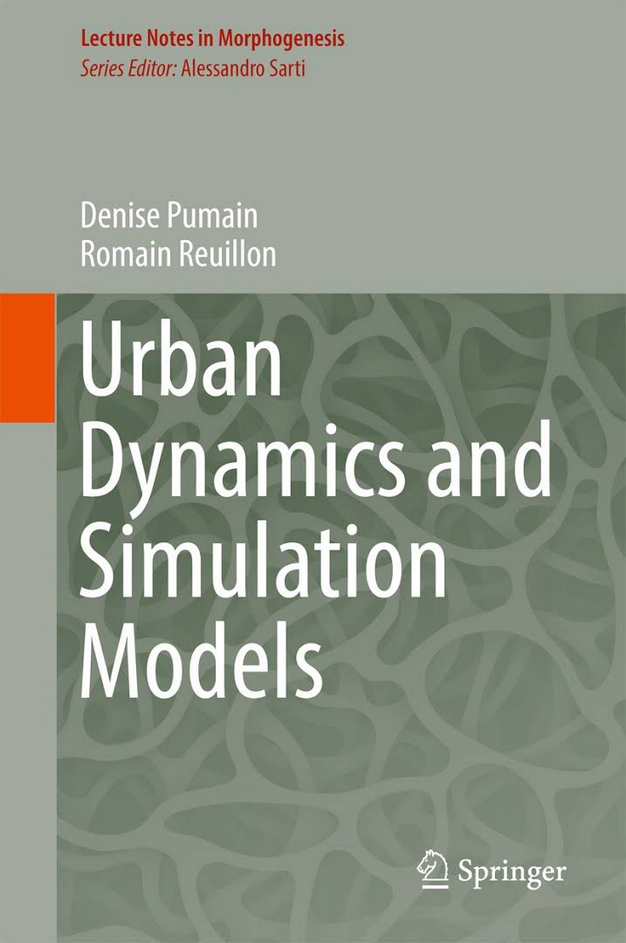
\includegraphics[width=\textwidth]{../20230629_IGN_BigData/figures/urban-dynamics-simulation-models-geodivercity.png}
\end{column}
\begin{column}{0.6\textwidth}
	Evolutionary urban theory \cite{pumain2018evolutionary}
	
	\medskip

	$\rightarrow$ Stylised facts on main systems of cities worldwide
	
	$\rightarrow$ Simulation models with an explicative function
	
	$\rightarrow$ Tools and model exploration methods: OpenMOLE mainly developed by R. Reuillon and M. Leclaire since 2008 at l'ISC-PIF
	
	\smallskip
	
	
	%
\includegraphics[width=\textwidth]{figures/openmole.png}
	% new logo!
	
\includegraphics[width=0.28\textwidth]{../20230629_IGN_BigData/figures/iconOM.png}
	
\includegraphics[width=0.68\textwidth]{../20230629_IGN_BigData/figures/openmole.png}
	
\end{column}
\end{columns}


}



\sframe{Scientific environment \cite{raimbault2018extracting}}{

\centering

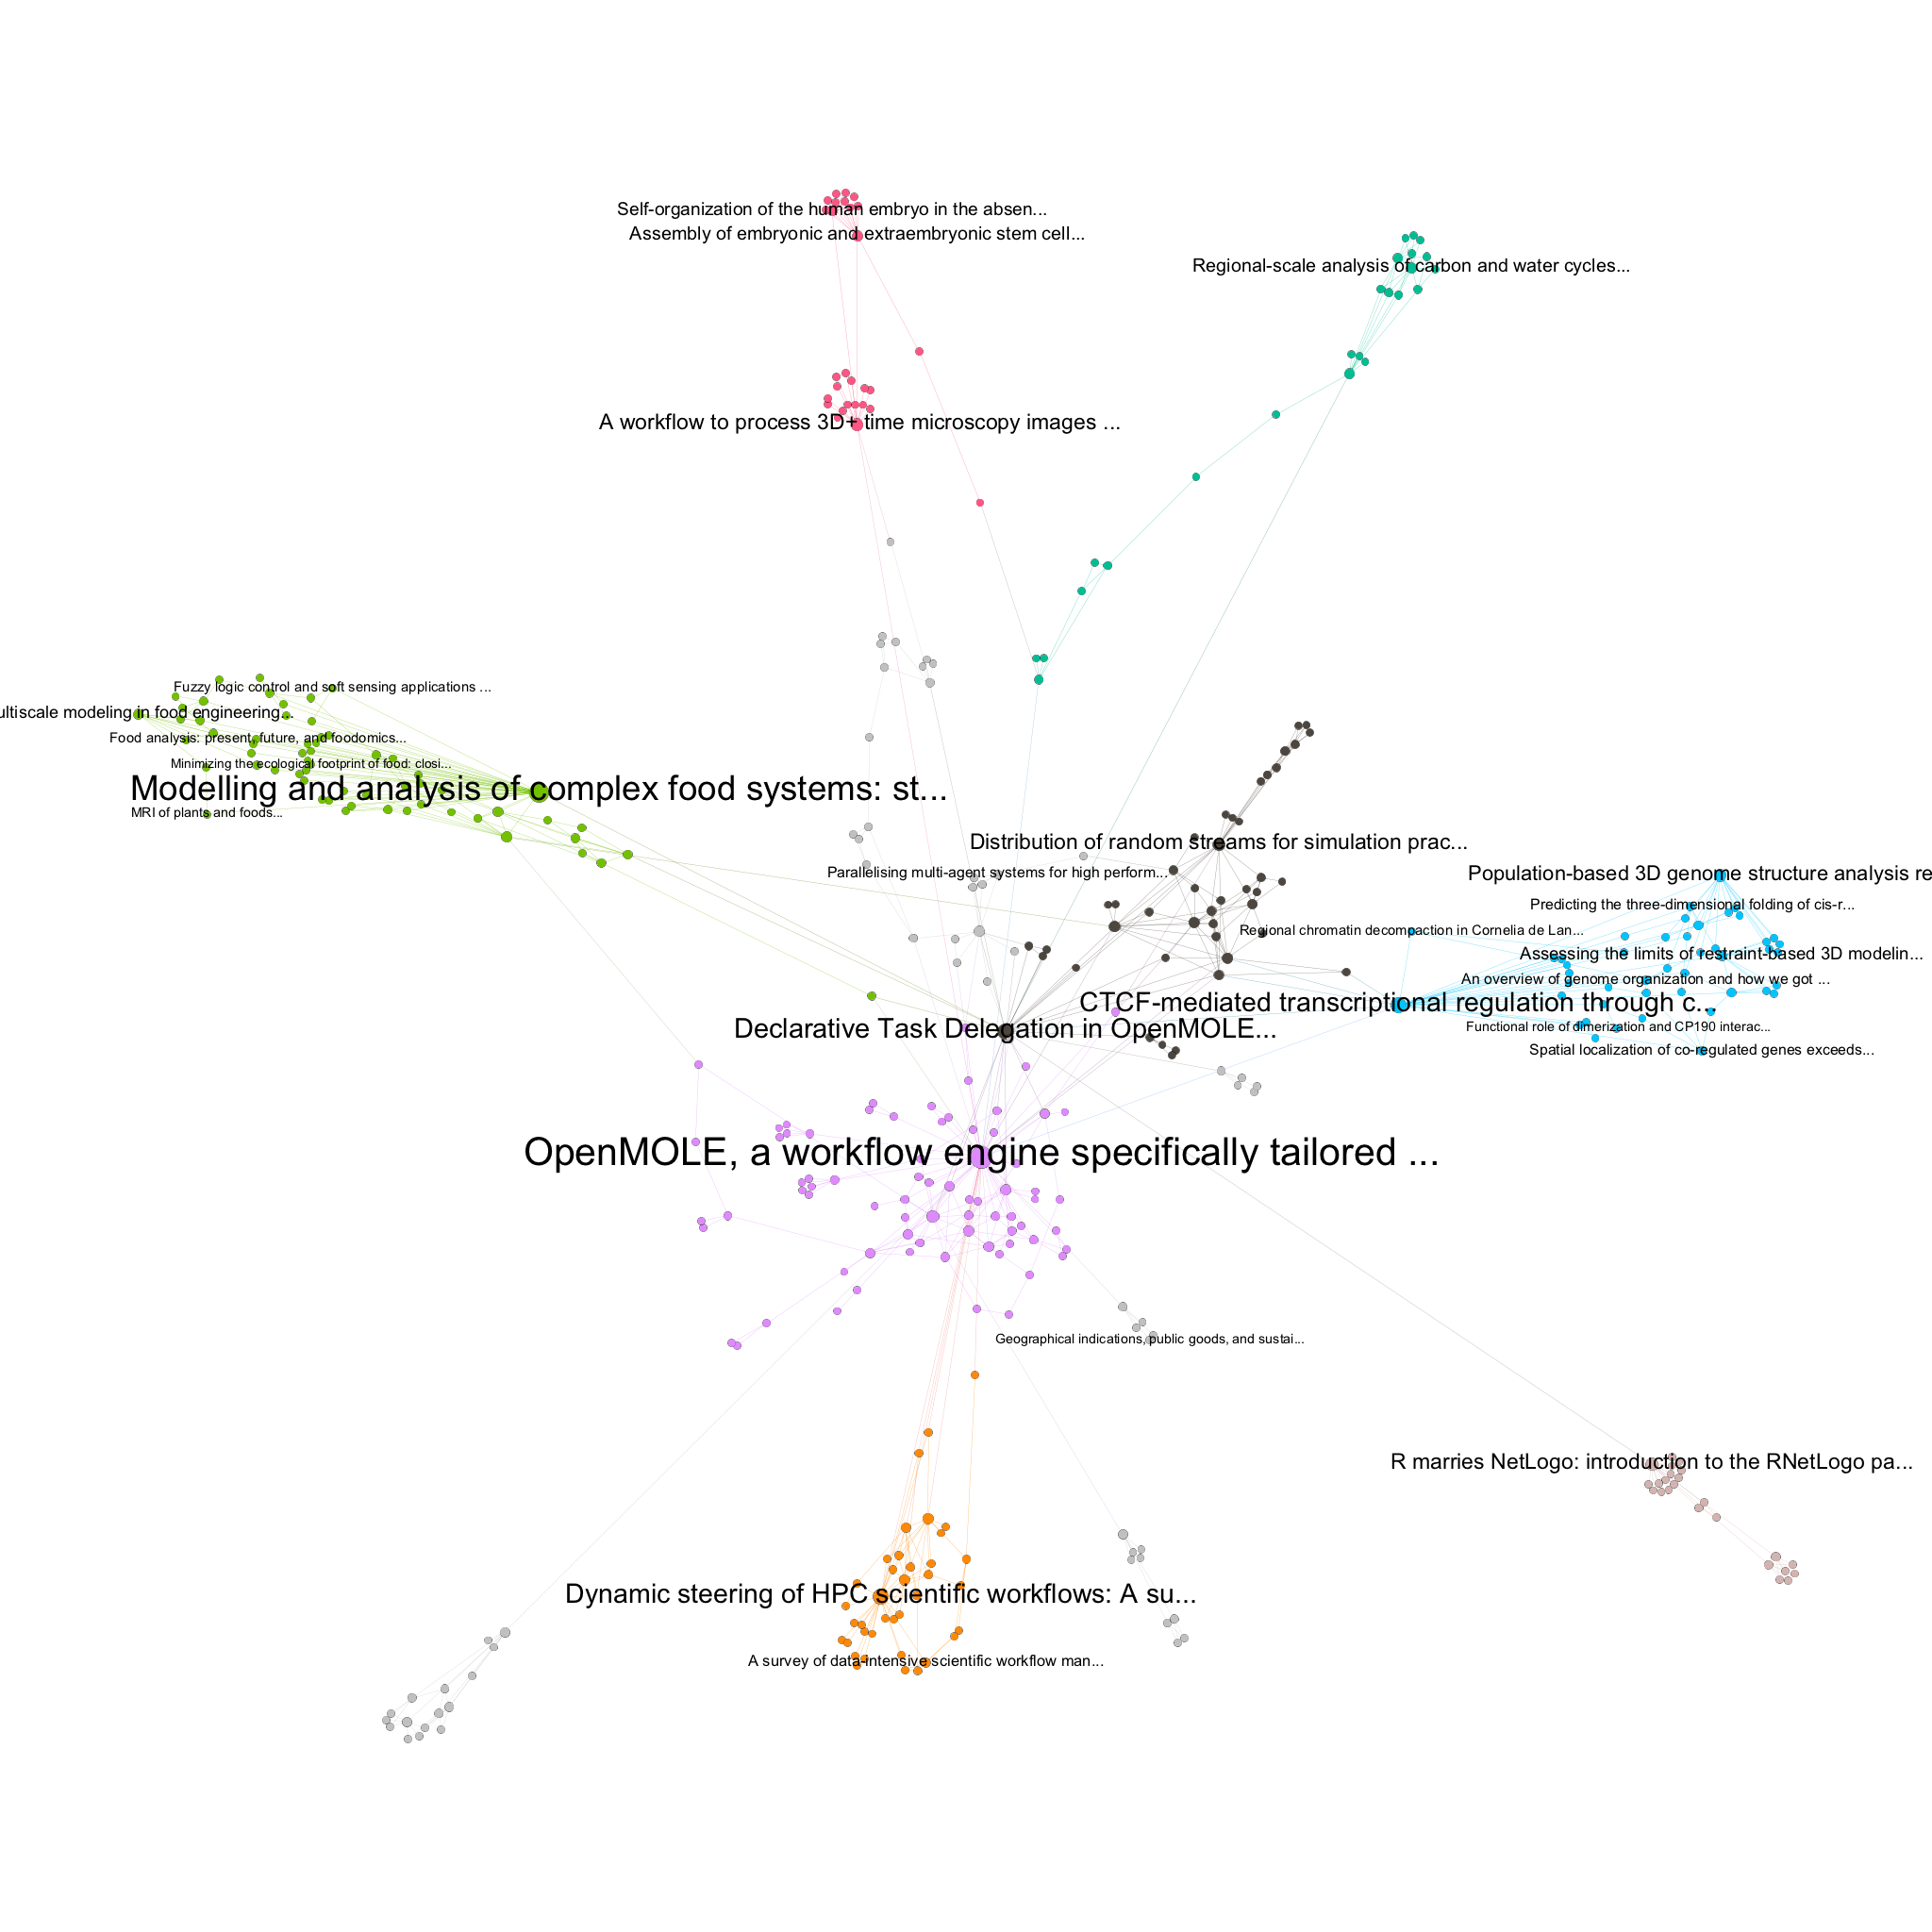
\includegraphics[width=\textwidth]{../20230629_IGN_BigData/figures/oml_depth3_core.png}
}


%\sframe{Méthodes et outils: OpenMOLE}{
%}

\sframe{OpenMOLE principles}{
	
	\footnotesize
	\textit{(i) State-of-the-art exploration and validation methods; (ii) Scaling with High Performance Computing; (iii) Model embedding.}
	
	\smallskip
	
	\centering
	
	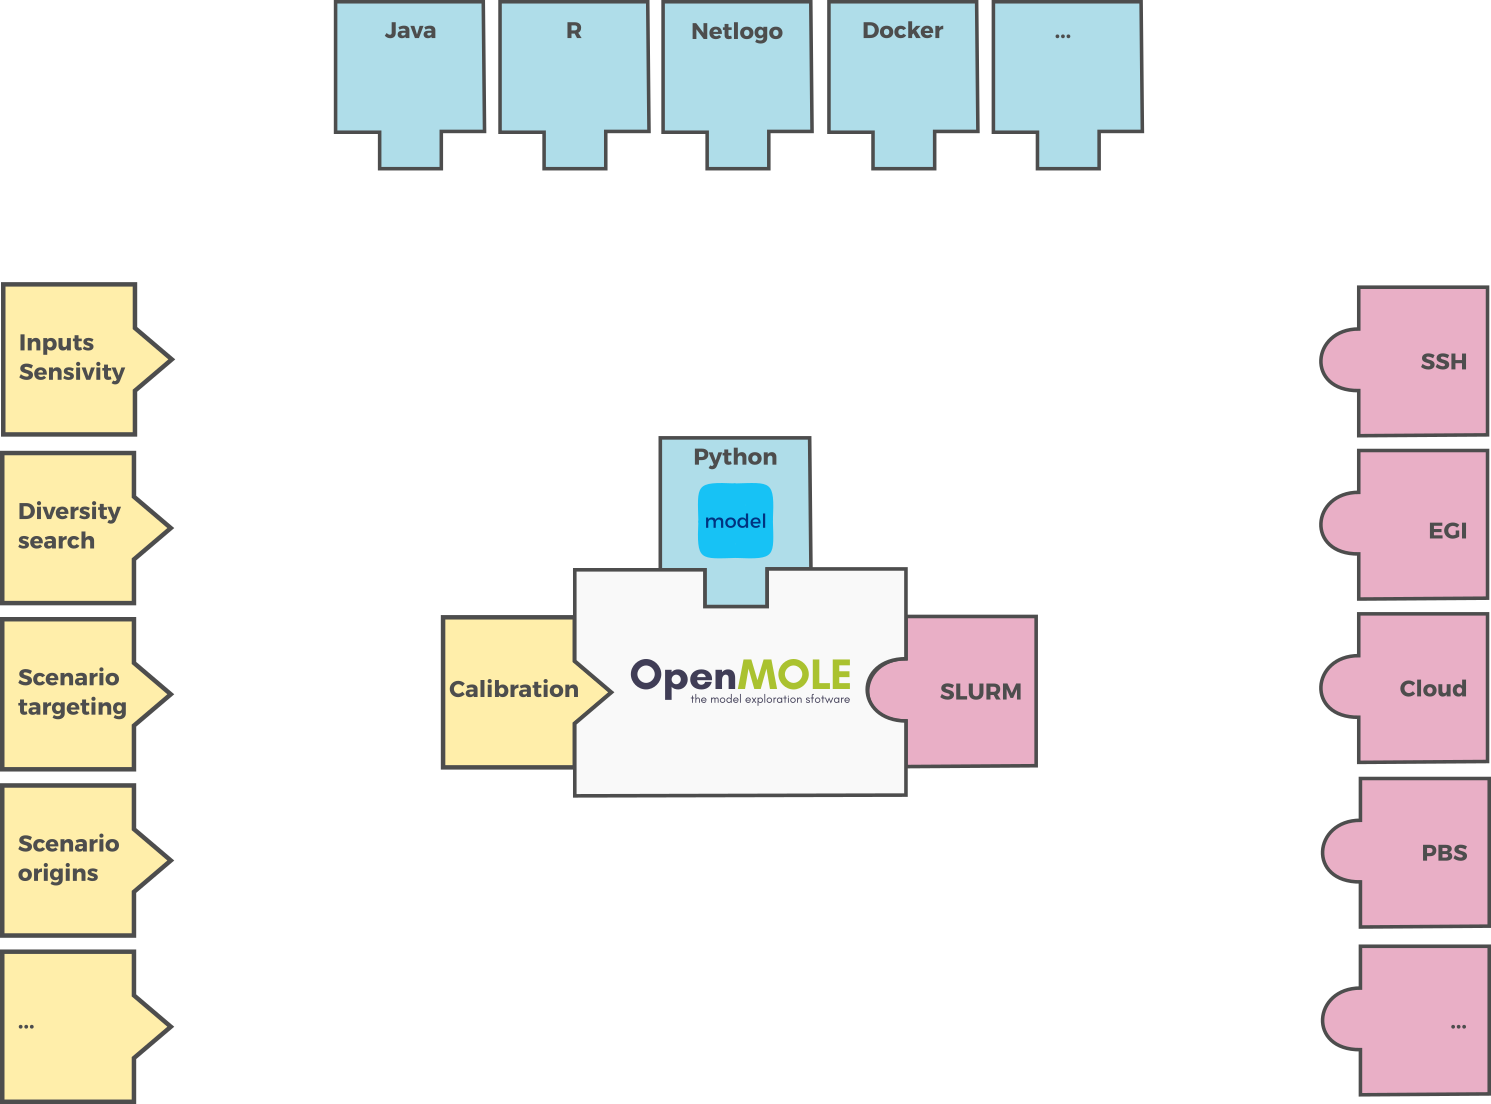
\includegraphics[width=0.9\textwidth]{../20230629_IGN_BigData/figures/openmole_axis.png}
	
}





\sframe{Web application interface}{

	\centering
	
	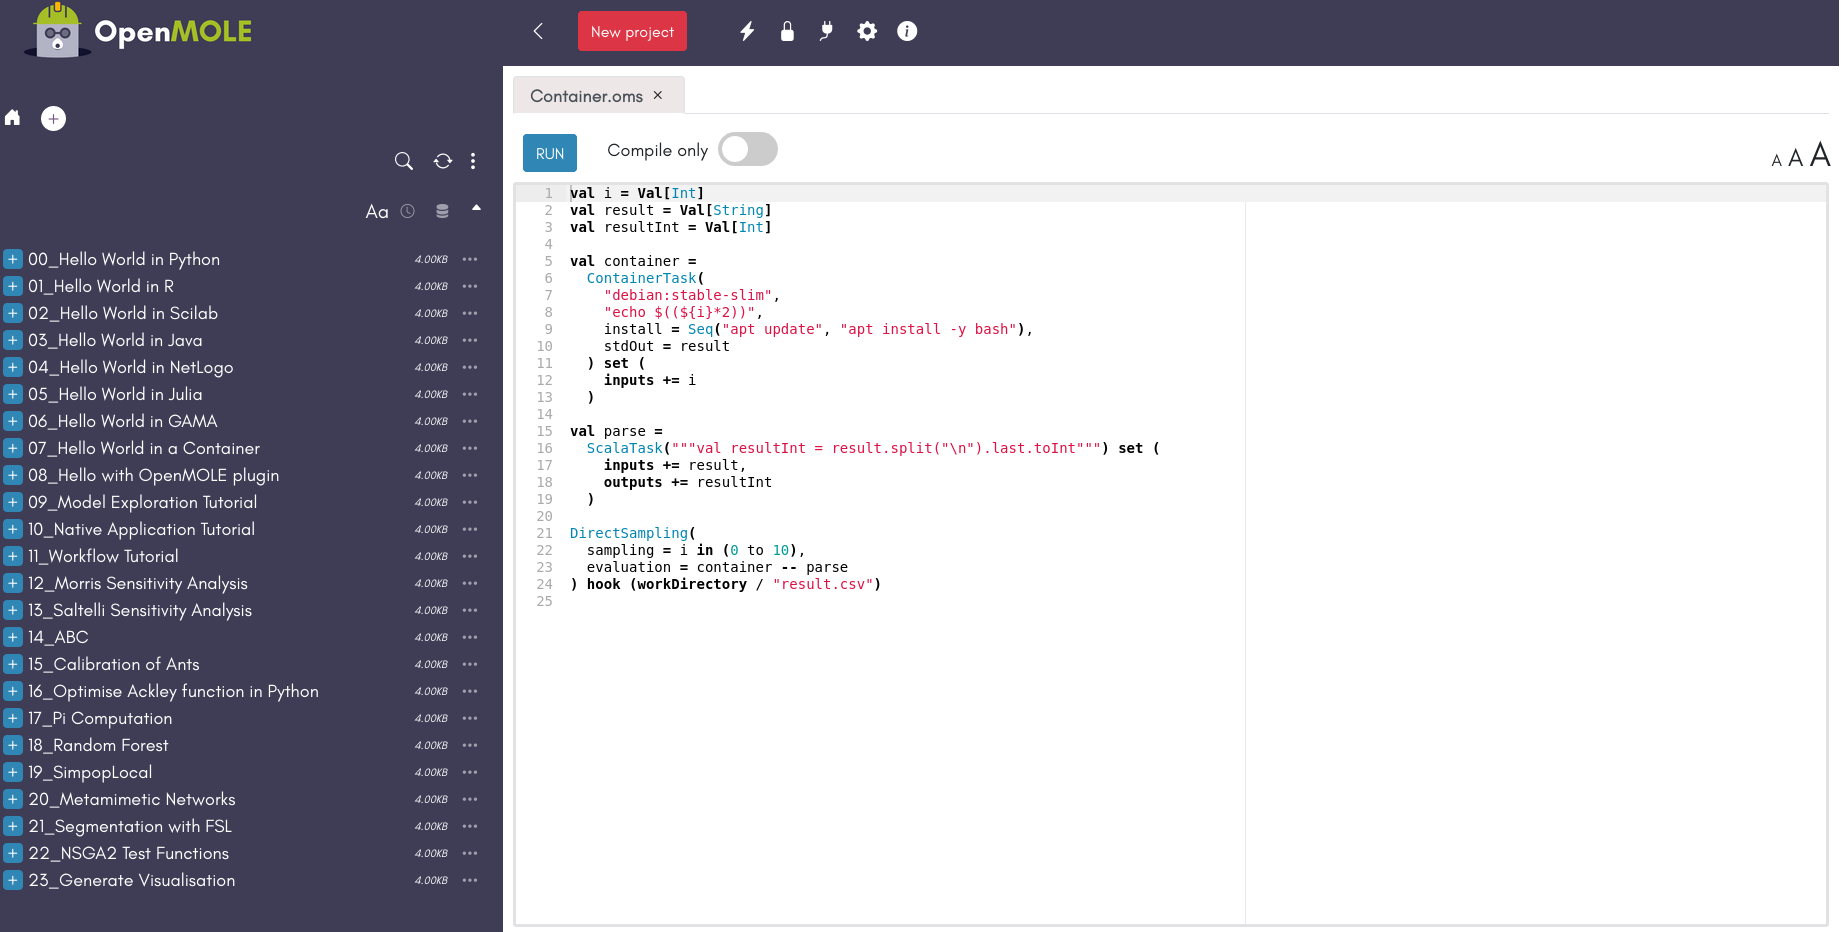
\includegraphics[width=\textwidth]{../20230629_IGN_BigData/figures/openmolefirefox.png}
	
}

\sframe{Simulation models}{

	\centering
	
	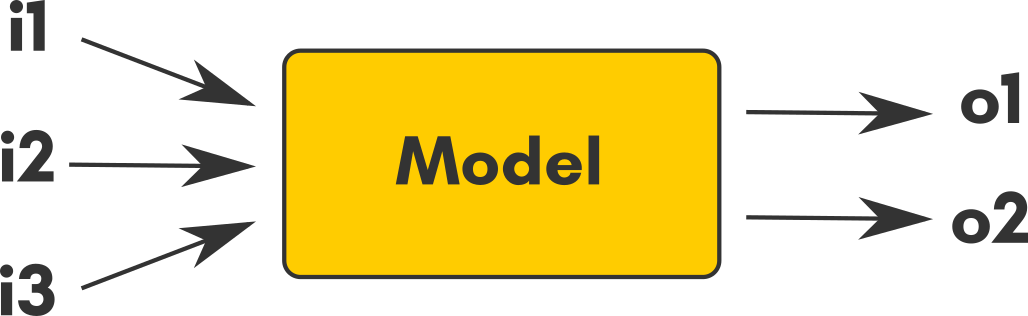
\includegraphics[width=\textwidth]{../20230629_IGN_BigData/figures/modelIO.png}

}



\sframe{Language agnosticity}{

	\centering
	
	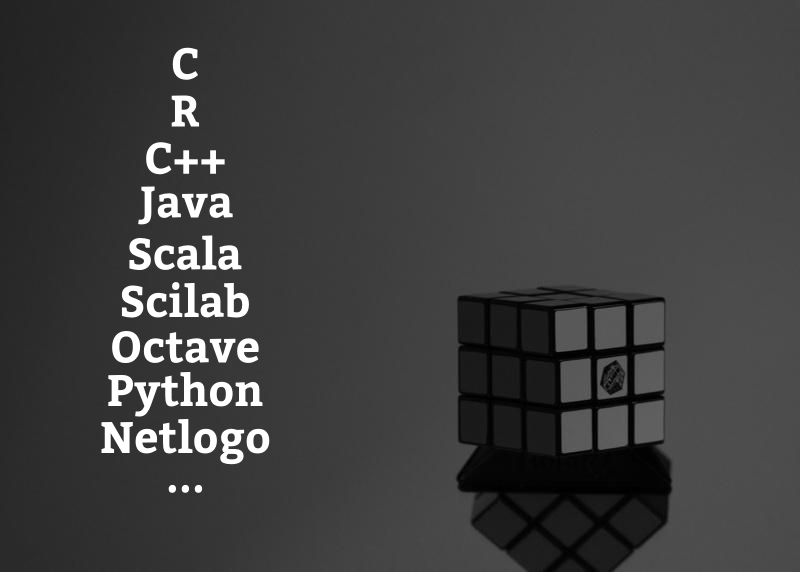
\includegraphics[width=\textwidth]{../20230629_IGN_BigData/figures/blackbox.png}

}

\sframe{Example: NetLogo model}{

	
	\begin{center}
	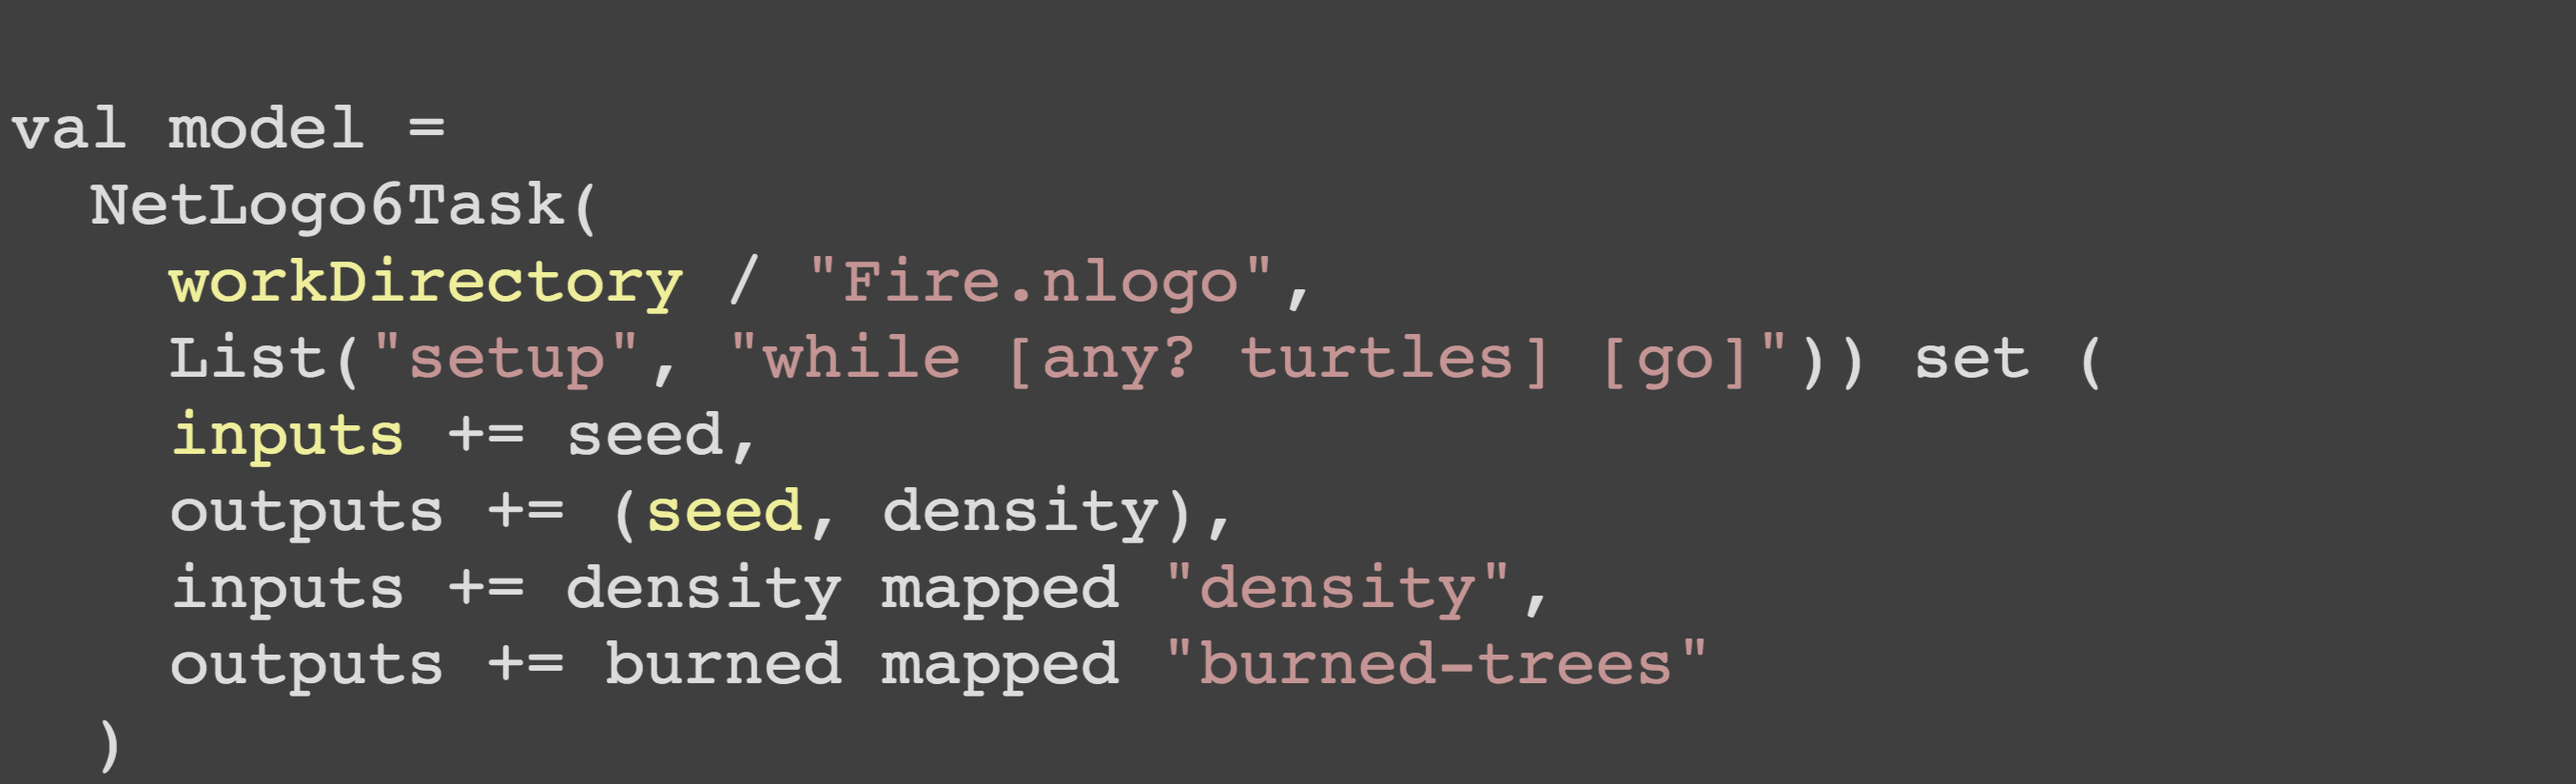
\includegraphics[width=\textwidth]{../20230629_IGN_BigData/figures/netlogomodel.png}
	\end{center}	
	
	\bigskip
	
	DSL based on scala for scripts
	
}

\sframe{R code}{

	
	\begin{center}
	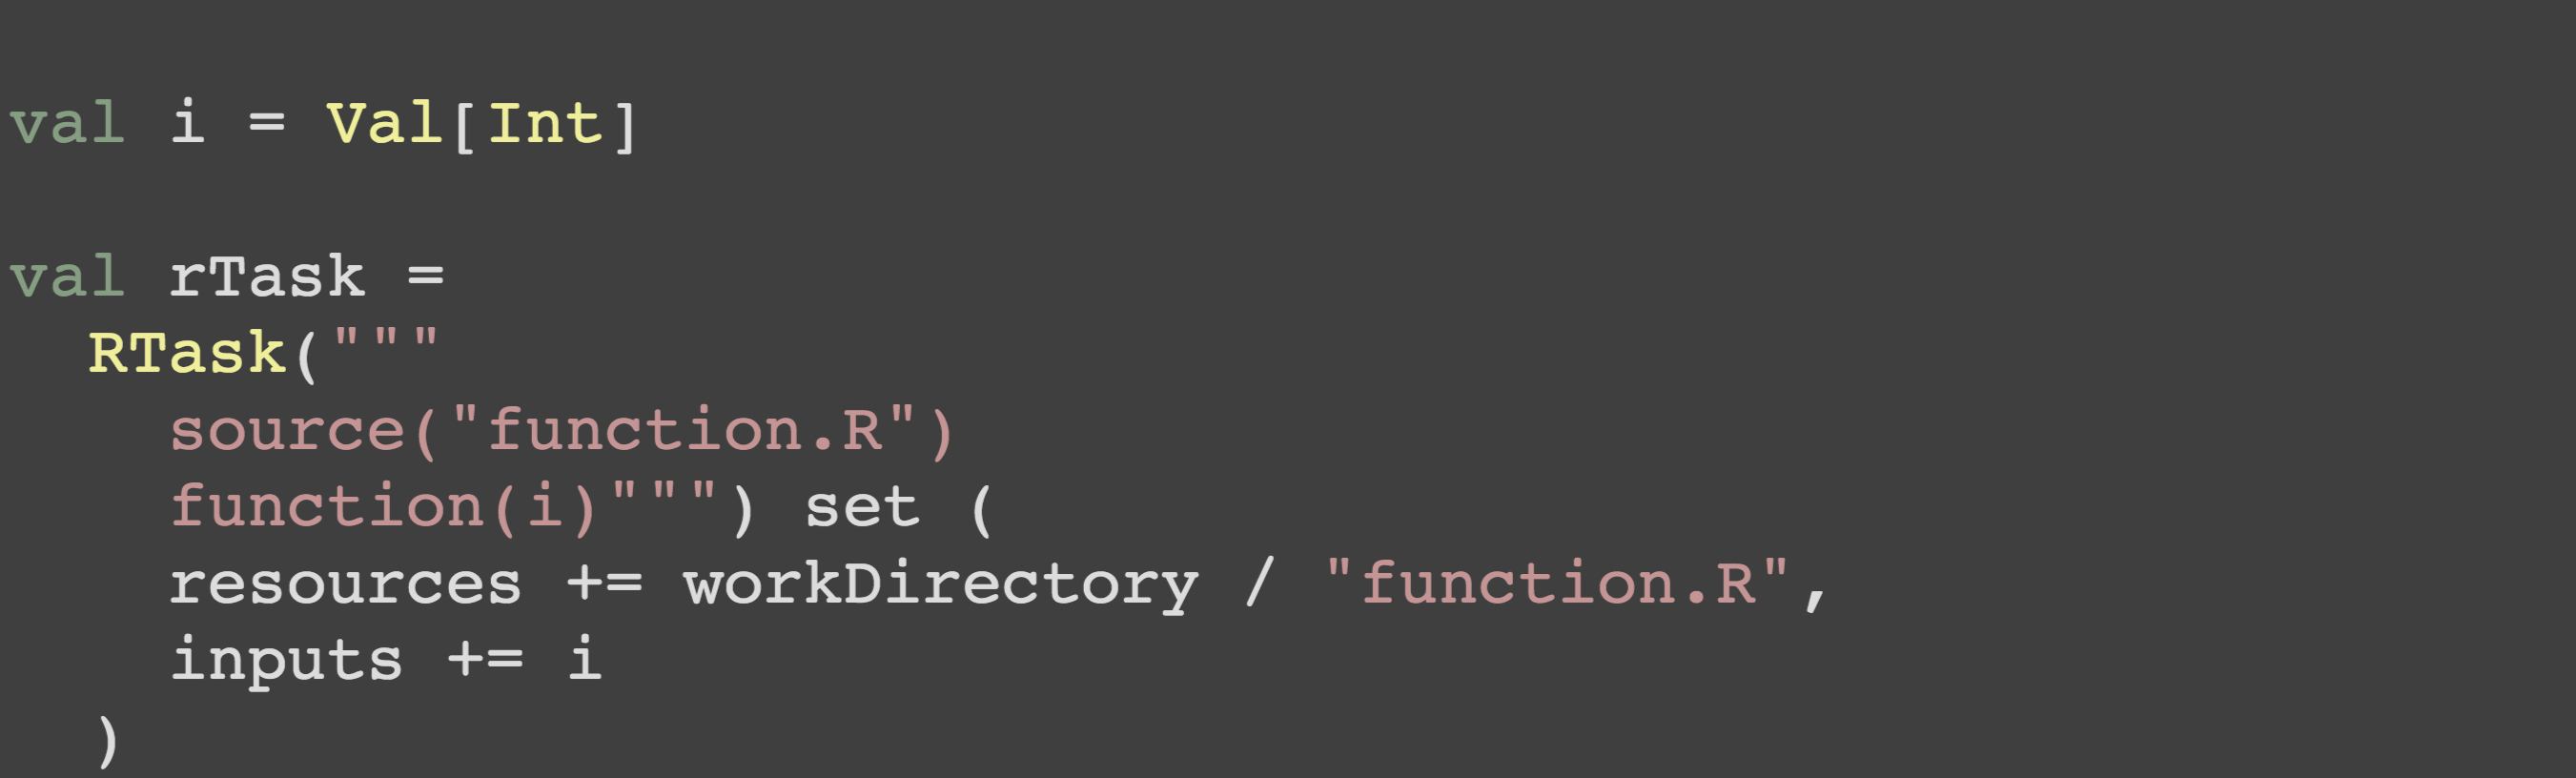
\includegraphics[width=\textwidth]{../20230629_IGN_BigData/figures/rcode.png}
	\end{center}	
	
	\bigskip
	
	Similar syntax for the \texttt{PythonTask}
	
}

\sframe{Docker container}{


	\begin{center}
	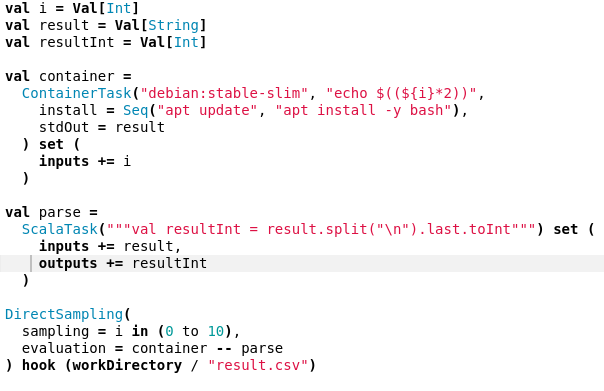
\includegraphics[width=\textwidth]{../20230629_IGN_BigData/figures/container.png}
	\end{center}	
	

}



\sframe{Methods}{
	
	\begin{itemize}
		\item Parameter estimation
		\item Sensitivity analysis
		\item Robustness analysis
		\item Optimisation
	\end{itemize}

	% Designed in a scalable manner, handle stochasticity, usable on any models and environments
	
	\medskip
	
	\textit{Designed to be scalable, to take stochasticity into account, to be usable on any model and computing environment.}
	
}

\sframe{Methods}{

	
	\begin{center}
	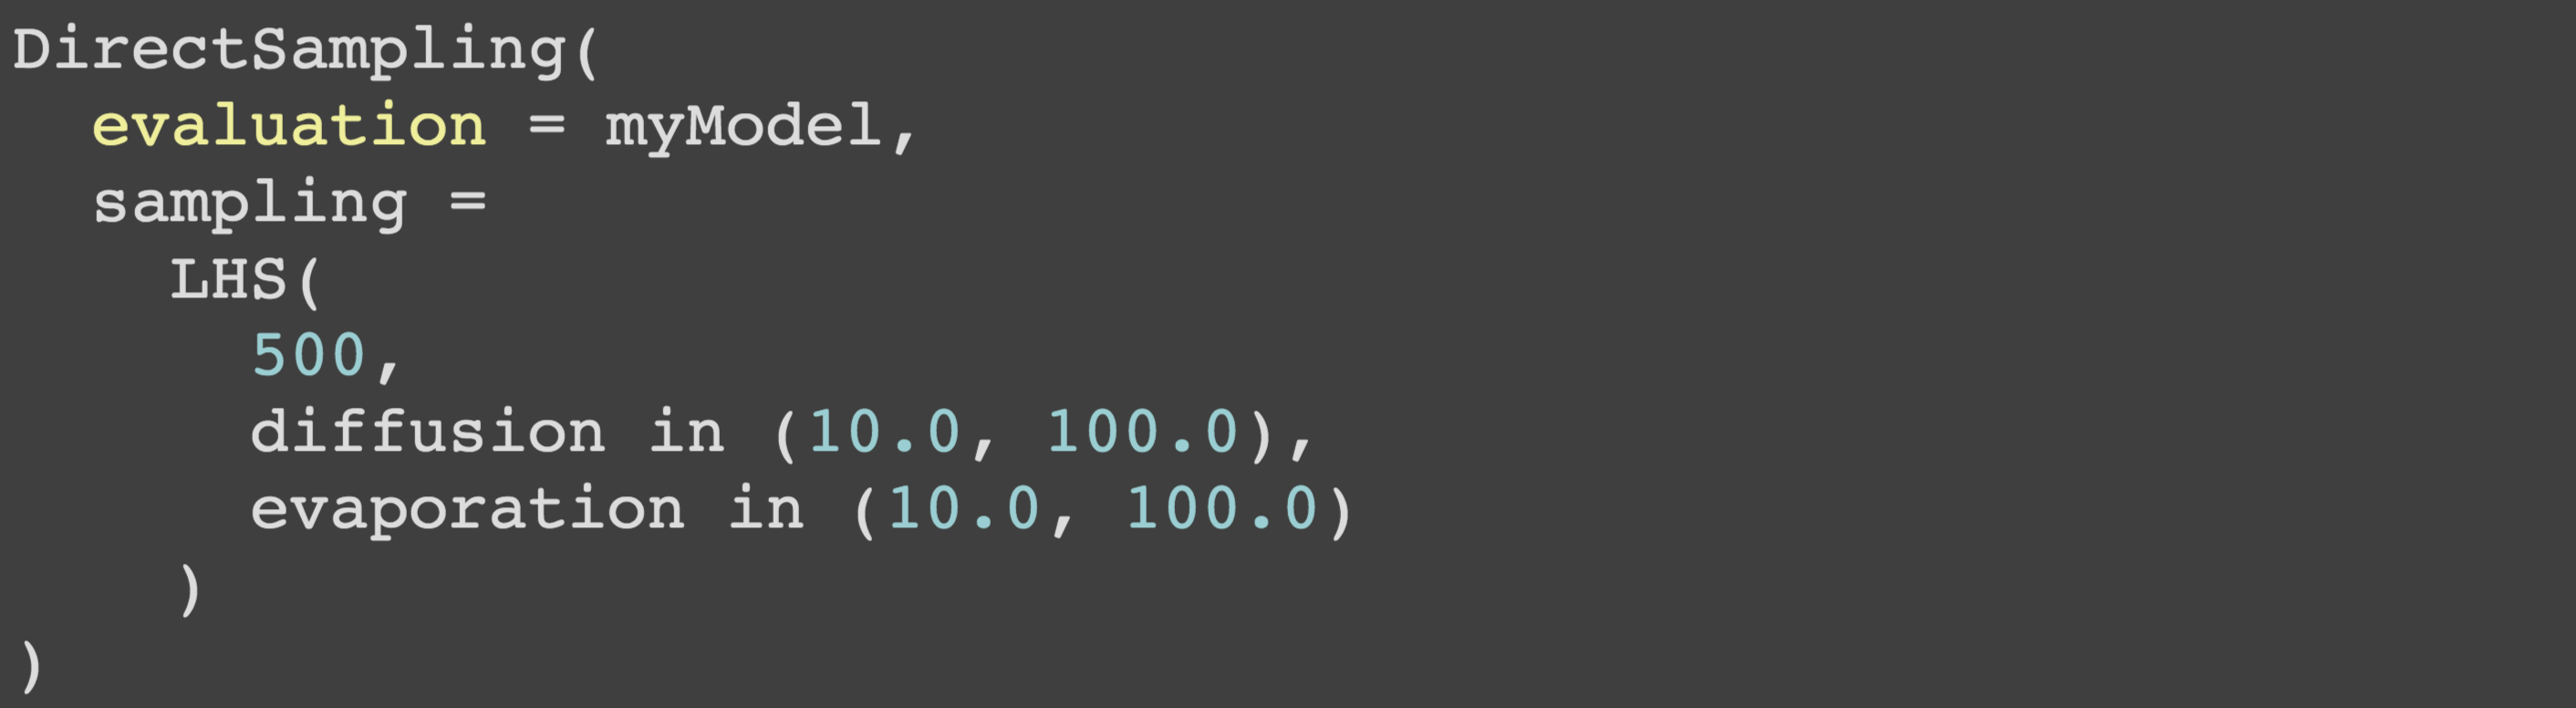
\includegraphics[width=\textwidth]{../20230629_IGN_BigData/figures/directsampling.png}
	\end{center}

	\bigskip
	
	Example of method syntax: explicit sampling

}




\sframe{Computing environment: up-scaling}{

% Prototype Small, Scale for Free

% Zero deployment approach
% No prior knowledge of remote environment needed
% No installation required on any machine
% User code and data are automatically deployed

\textit{Local prototypes, transparent scaling.}

\bigskip

	\centering
	
	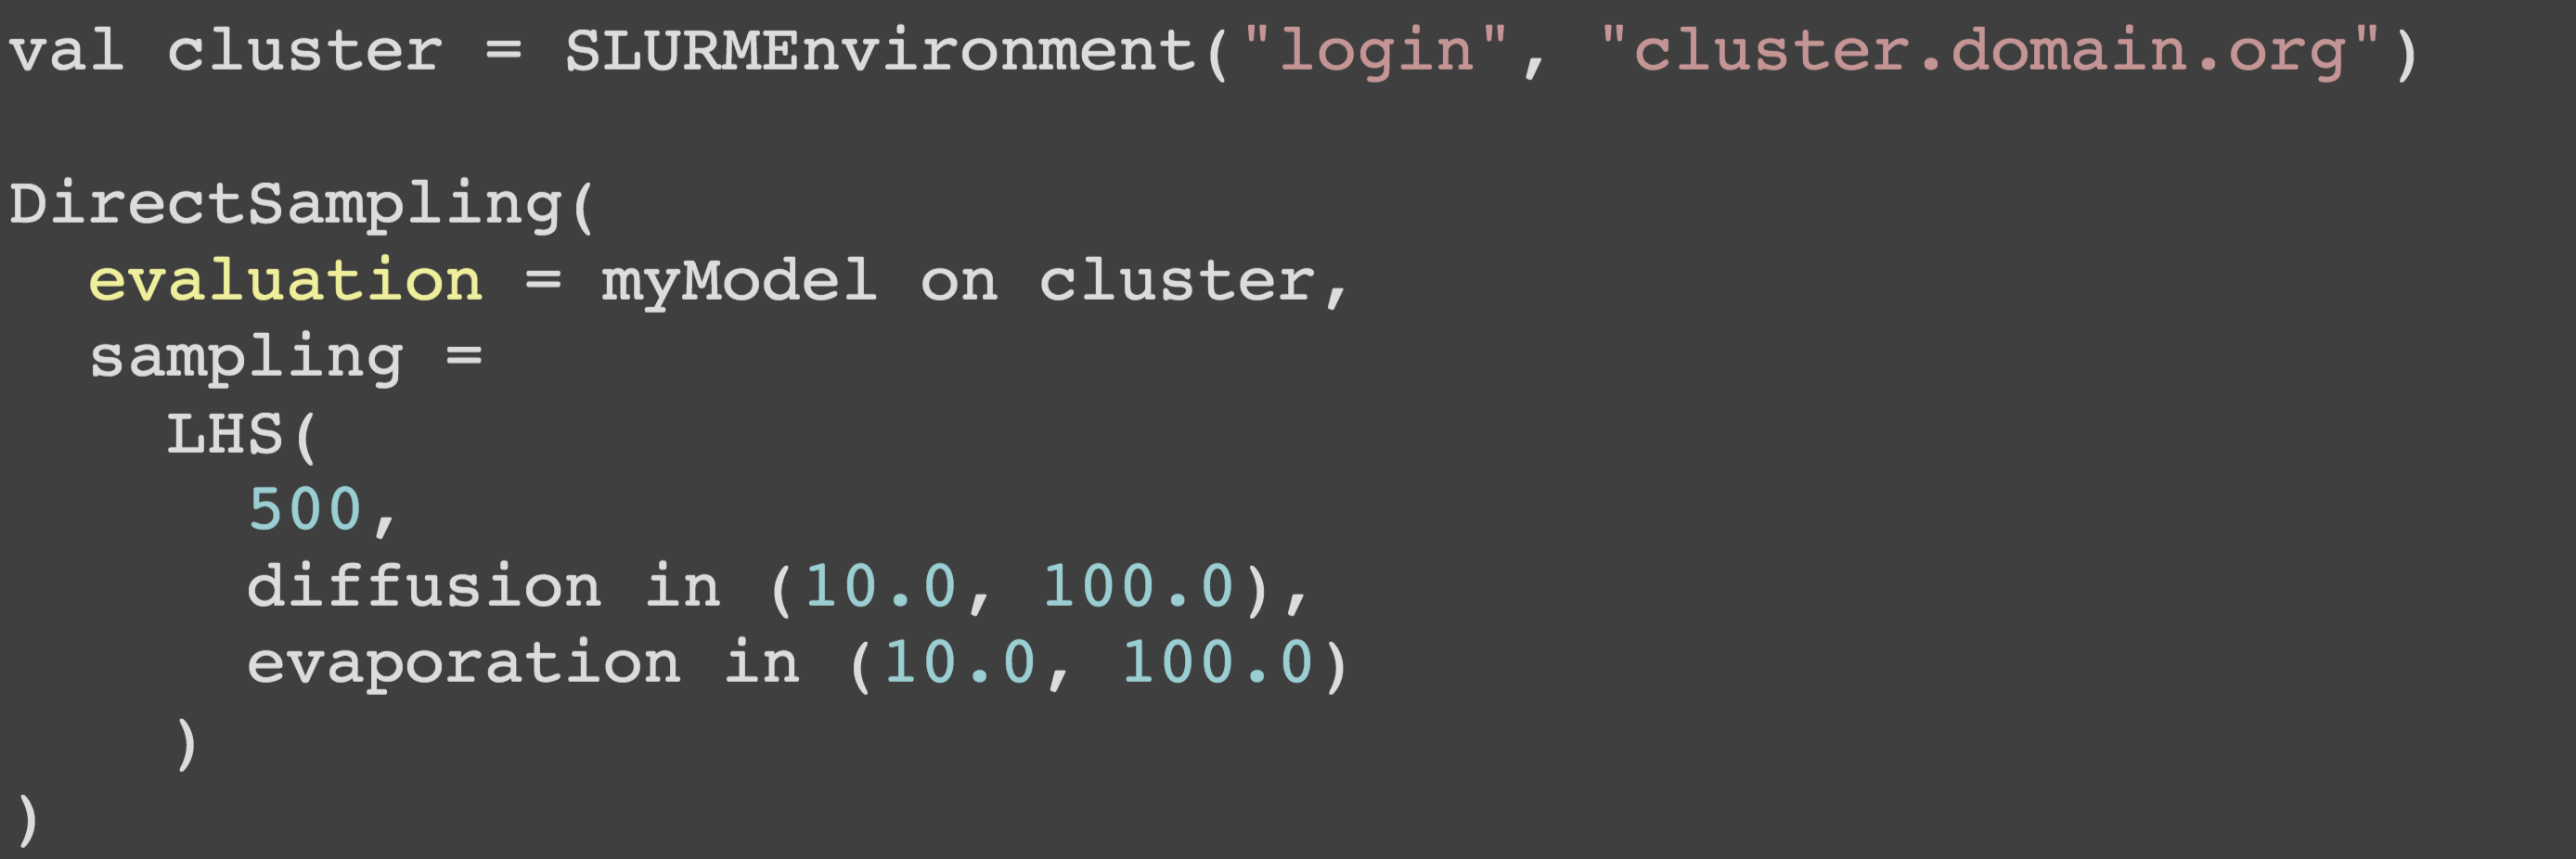
\includegraphics[width=\textwidth]{../20230629_IGN_BigData/figures/cluster.png}

}

\sframe{Computing environment}{


\begin{itemize}
	\item Multi-thread
	\item Delegation through SSH
	\item PBS
	\item SLURM
	\item Condor
	\item SGE
	\item OAR
	\item EGI Grid
\end{itemize}



}




\sframe{Theories and model evalution}{

	{\centering
	
	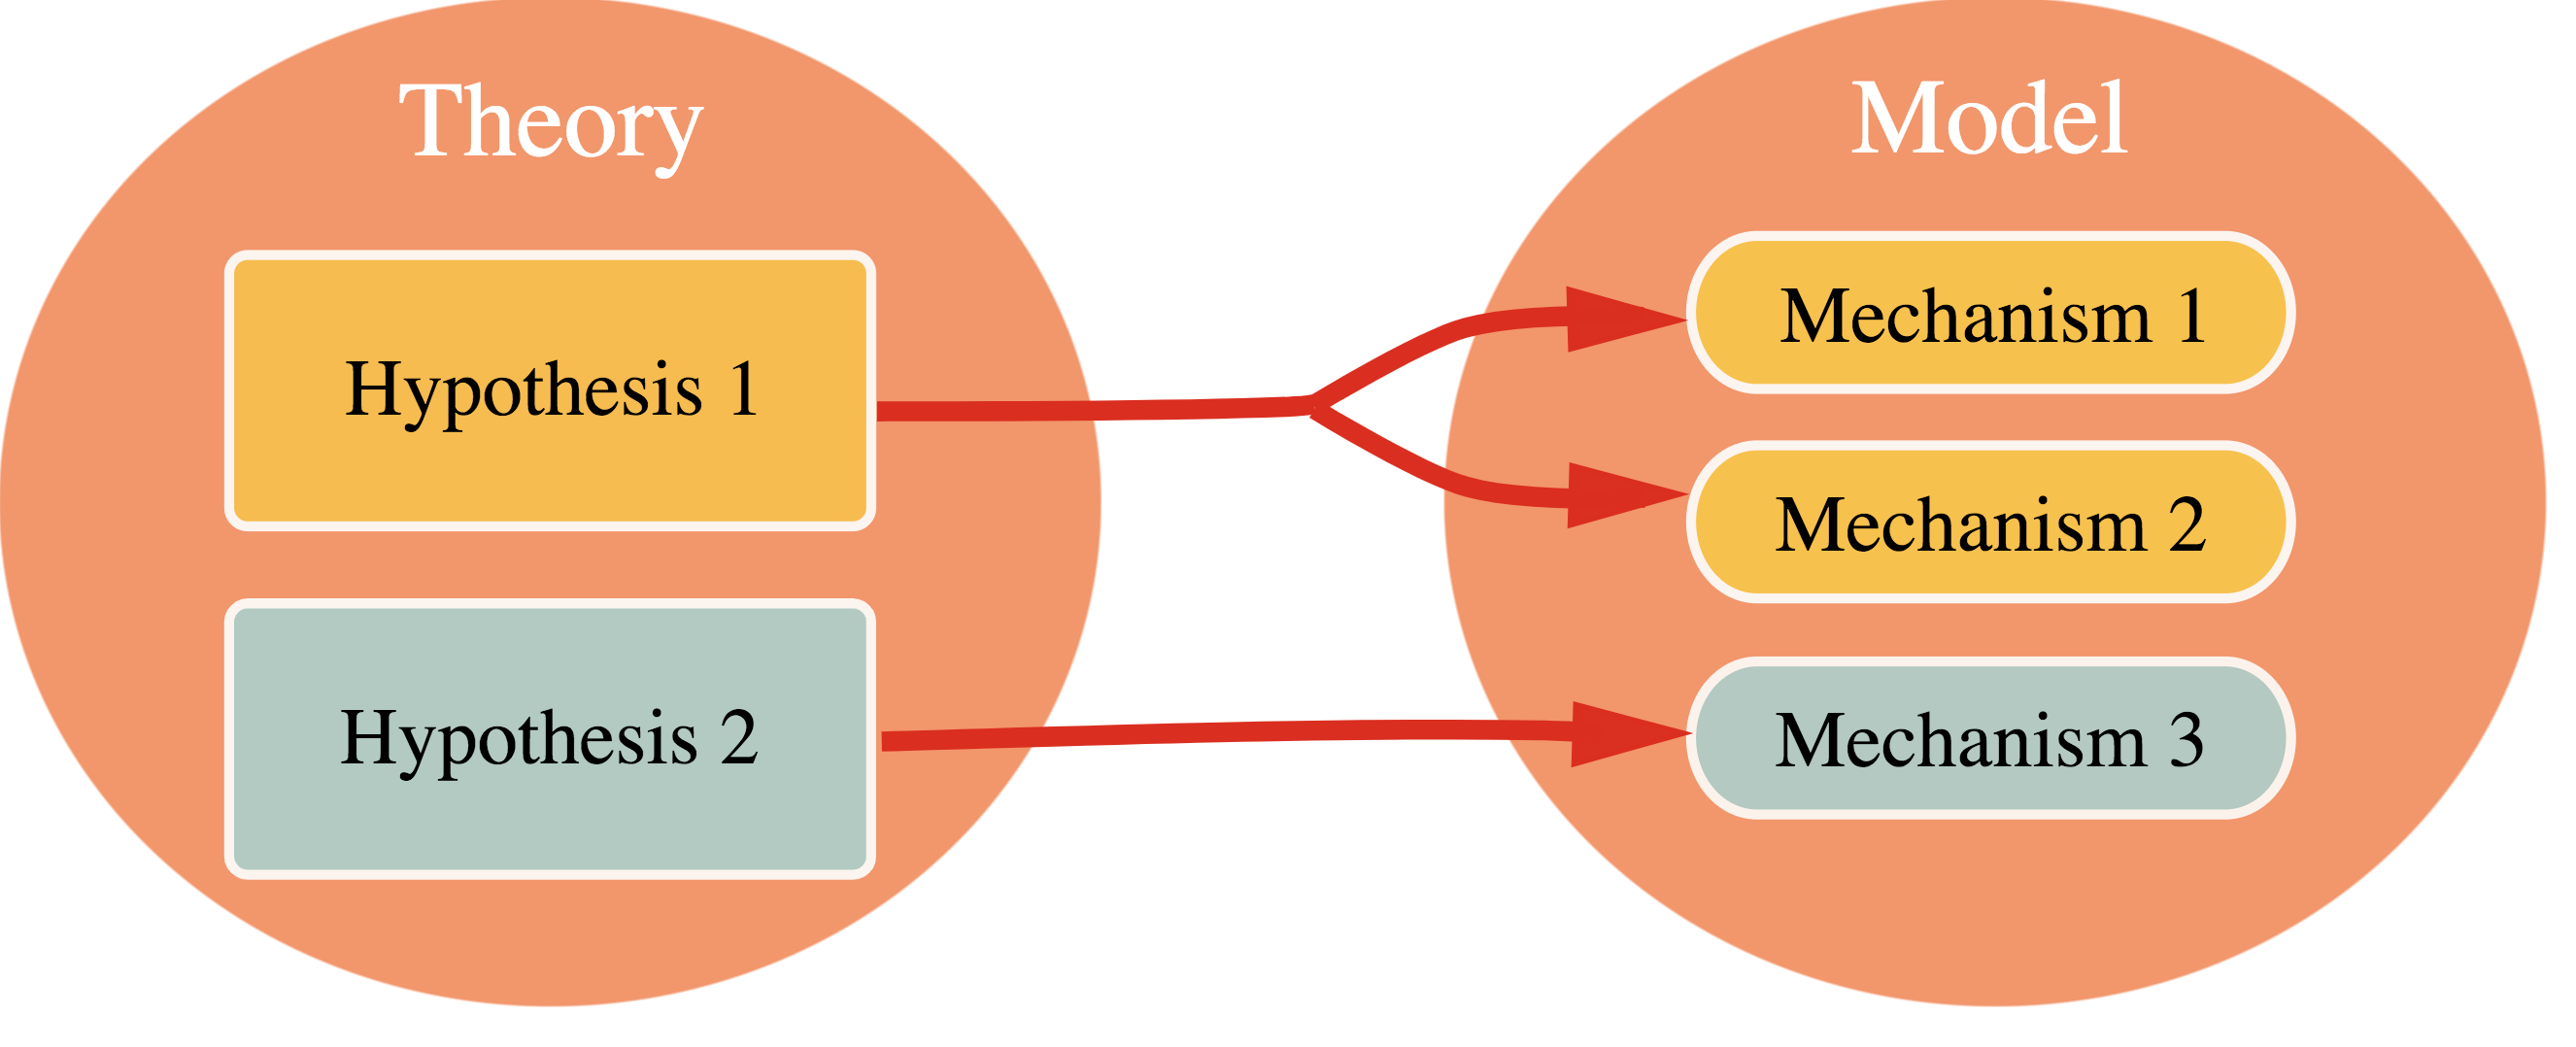
\includegraphics[width=\textwidth]{../20230629_IGN_BigData/figures/descriptivemodel.png}
}

%Descriptive models
%Design/evaluate a theory involving causal effects through its capacity to (re-)produce some patterns/data.

\textit{Construct and evaluate a theory implying causal mechanisms.}


\medskip

%Model evaluation
%How to assess:

\textbf{Evaluation: } How to ensure

\begin{enumerate}
	\item the sufficiency of the mechanisms ?
	\item the necessity of the mechanisms ?
	\item the uniqueness of the mechanisms ?
\end{enumerate}
%


}




\sframe{Sufficiency \cite{schmitt2014half}}{

Classical approach: parameter space sampling (ex. Sobol) $\rightarrow$ large dataset produced and parameter space remains unexplored.

\bigskip

\textit{Inverse approach: from outputs to parameters}

\medskip

%
\textit{Formalising the expectations: }

	\begin{center}
	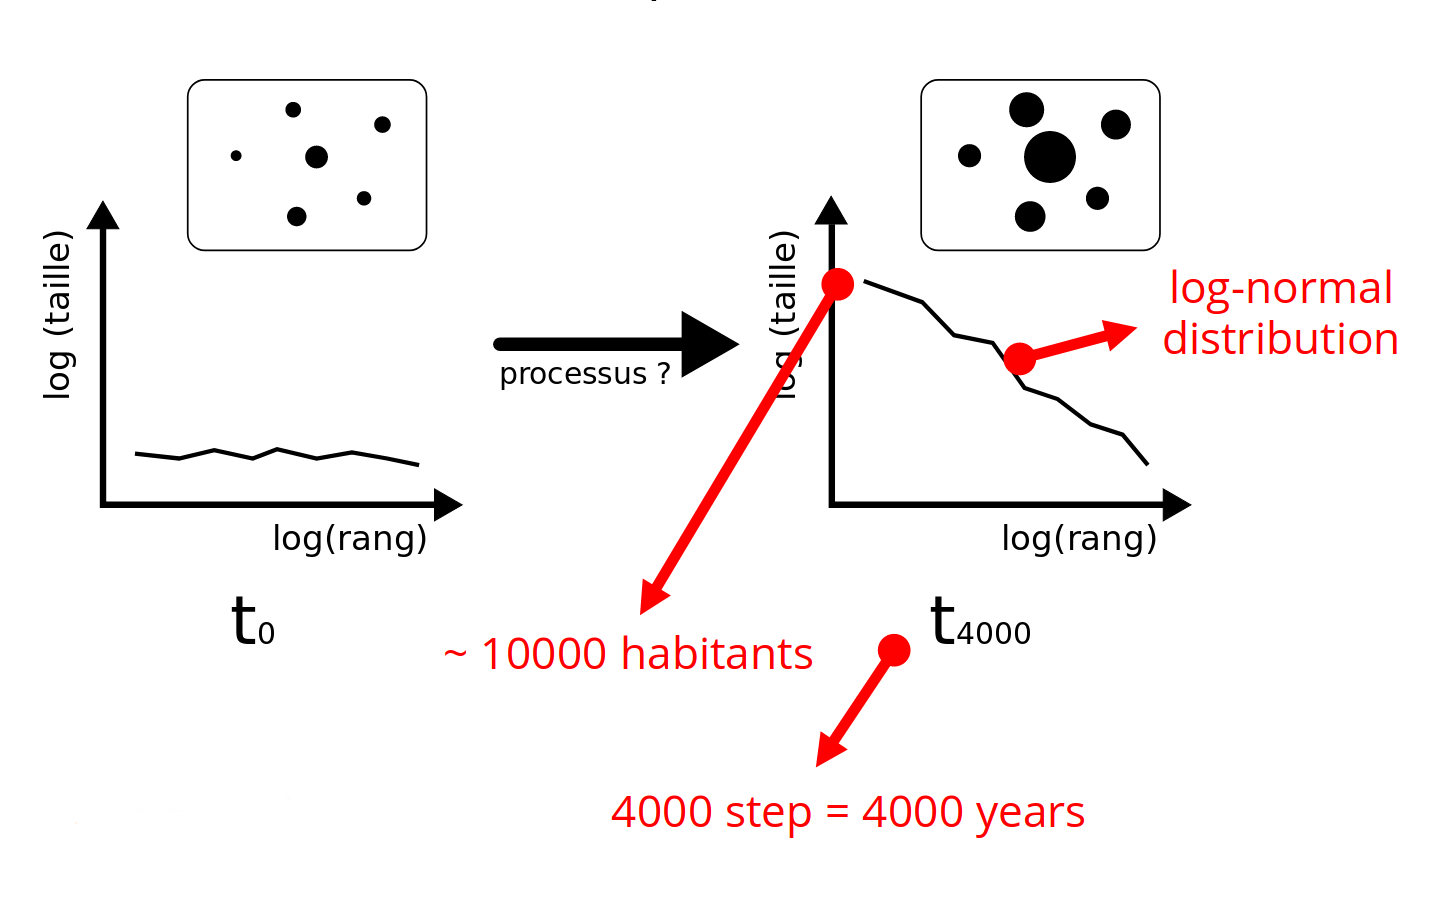
\includegraphics[width=\textwidth]{../20230629_IGN_BigData/figures/slocal_fitness.png}
	\end{center}

\bigskip

$\rightarrow$ multi-objective minimisation using a NSGA2 genetic algorithm
	

}




\sframe{Calibration results}{
	
	%.
	\textit{No compromise between the 3 objectives.}

\medskip

	{\centering
	
	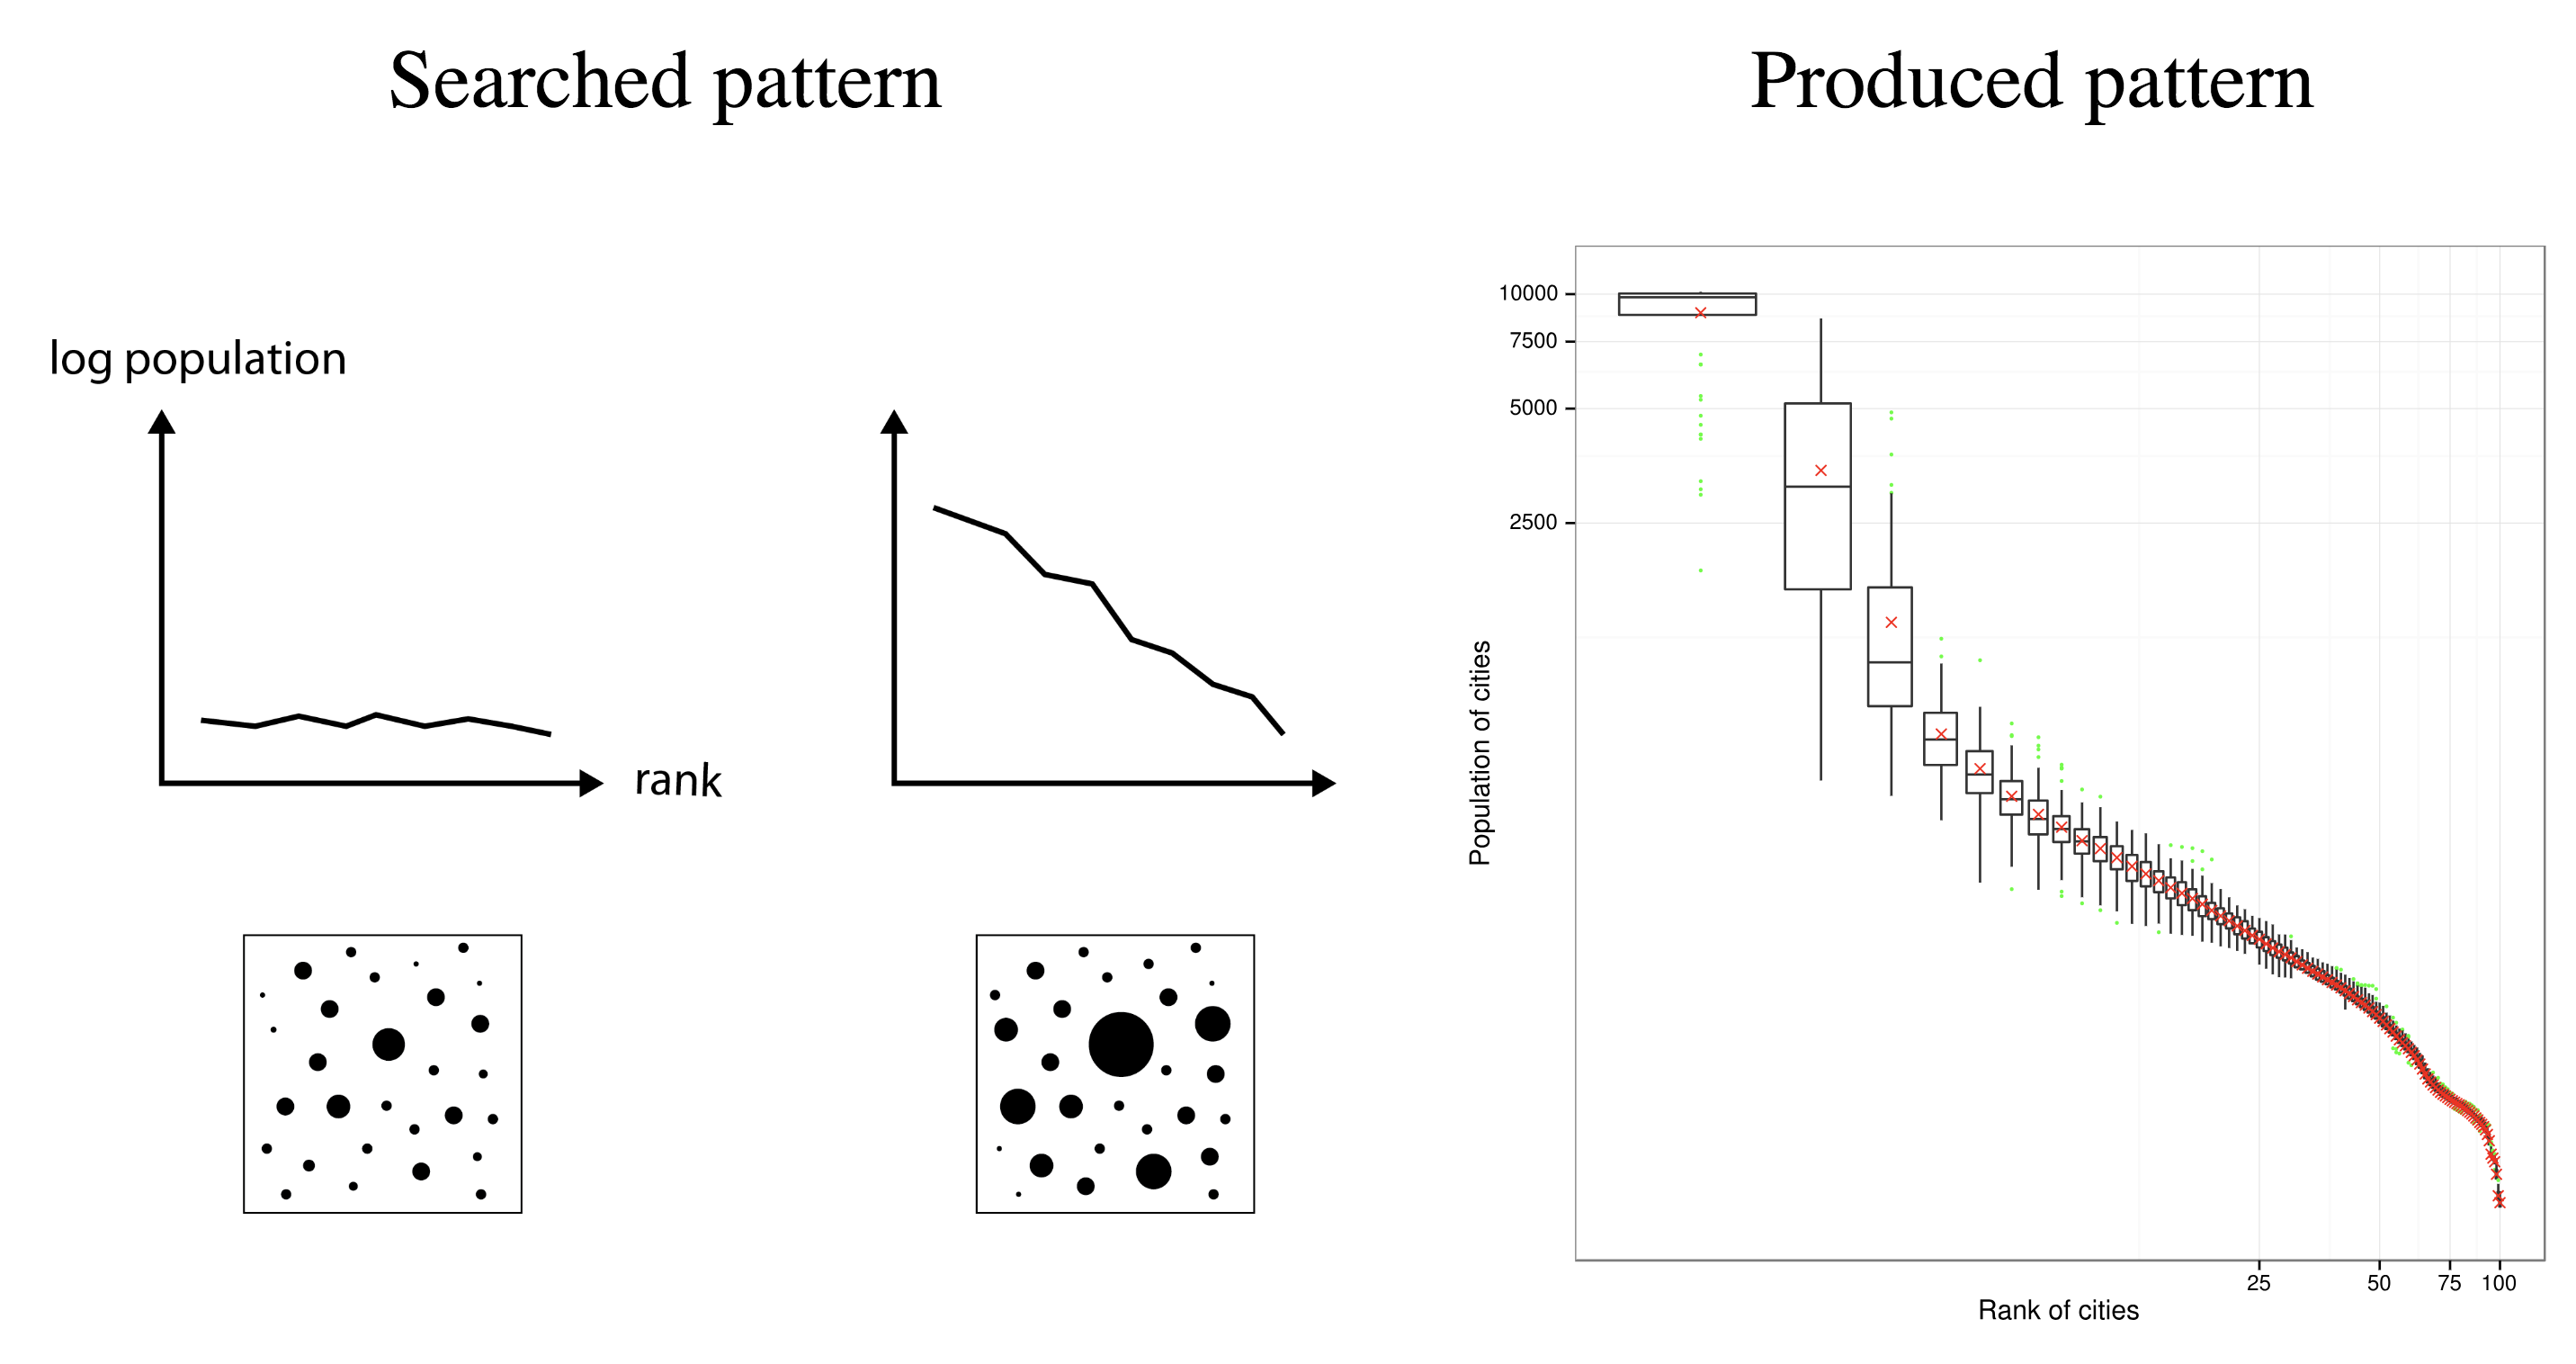
\includegraphics[width=\textwidth]{../20230629_IGN_BigData/figures/slocalcalib.png}
	}
	
%	Evaluation approach
%Would not have been found using a direct method.


%

\medskip

The method is tractable (even for ABMs): Handles stochasticity: 100x gain; Support for distributed computing: 1000x gain.

%Conclusion
%How to assess:

%the sufficiency of the mechanisms Y
%the necessity of the mechanisms ?
%the uniqueness of the mechanisms ?

}


\sframe{Necessity \cite{reuillon2015}}{

%
%

%
%
\textbf{A new algorithm}

\medskip

\begin{enumerate}
	\item To detect if a parameter is useful: it impacts the capacity of the model to produce plausible outcomes.
	\item To better constrain the parameter ranges.
	\item As an indirect way to detect if some of the mechanisms are expandable
\end{enumerate}


%Objective
%Hundreds of calibrations

	%\centering
	
	%\includegraphics[width=\textwidth]{figures/PdiffusionZ.pdf.png}


}

\sframe{Profile algorithm}{
{\centering
	
	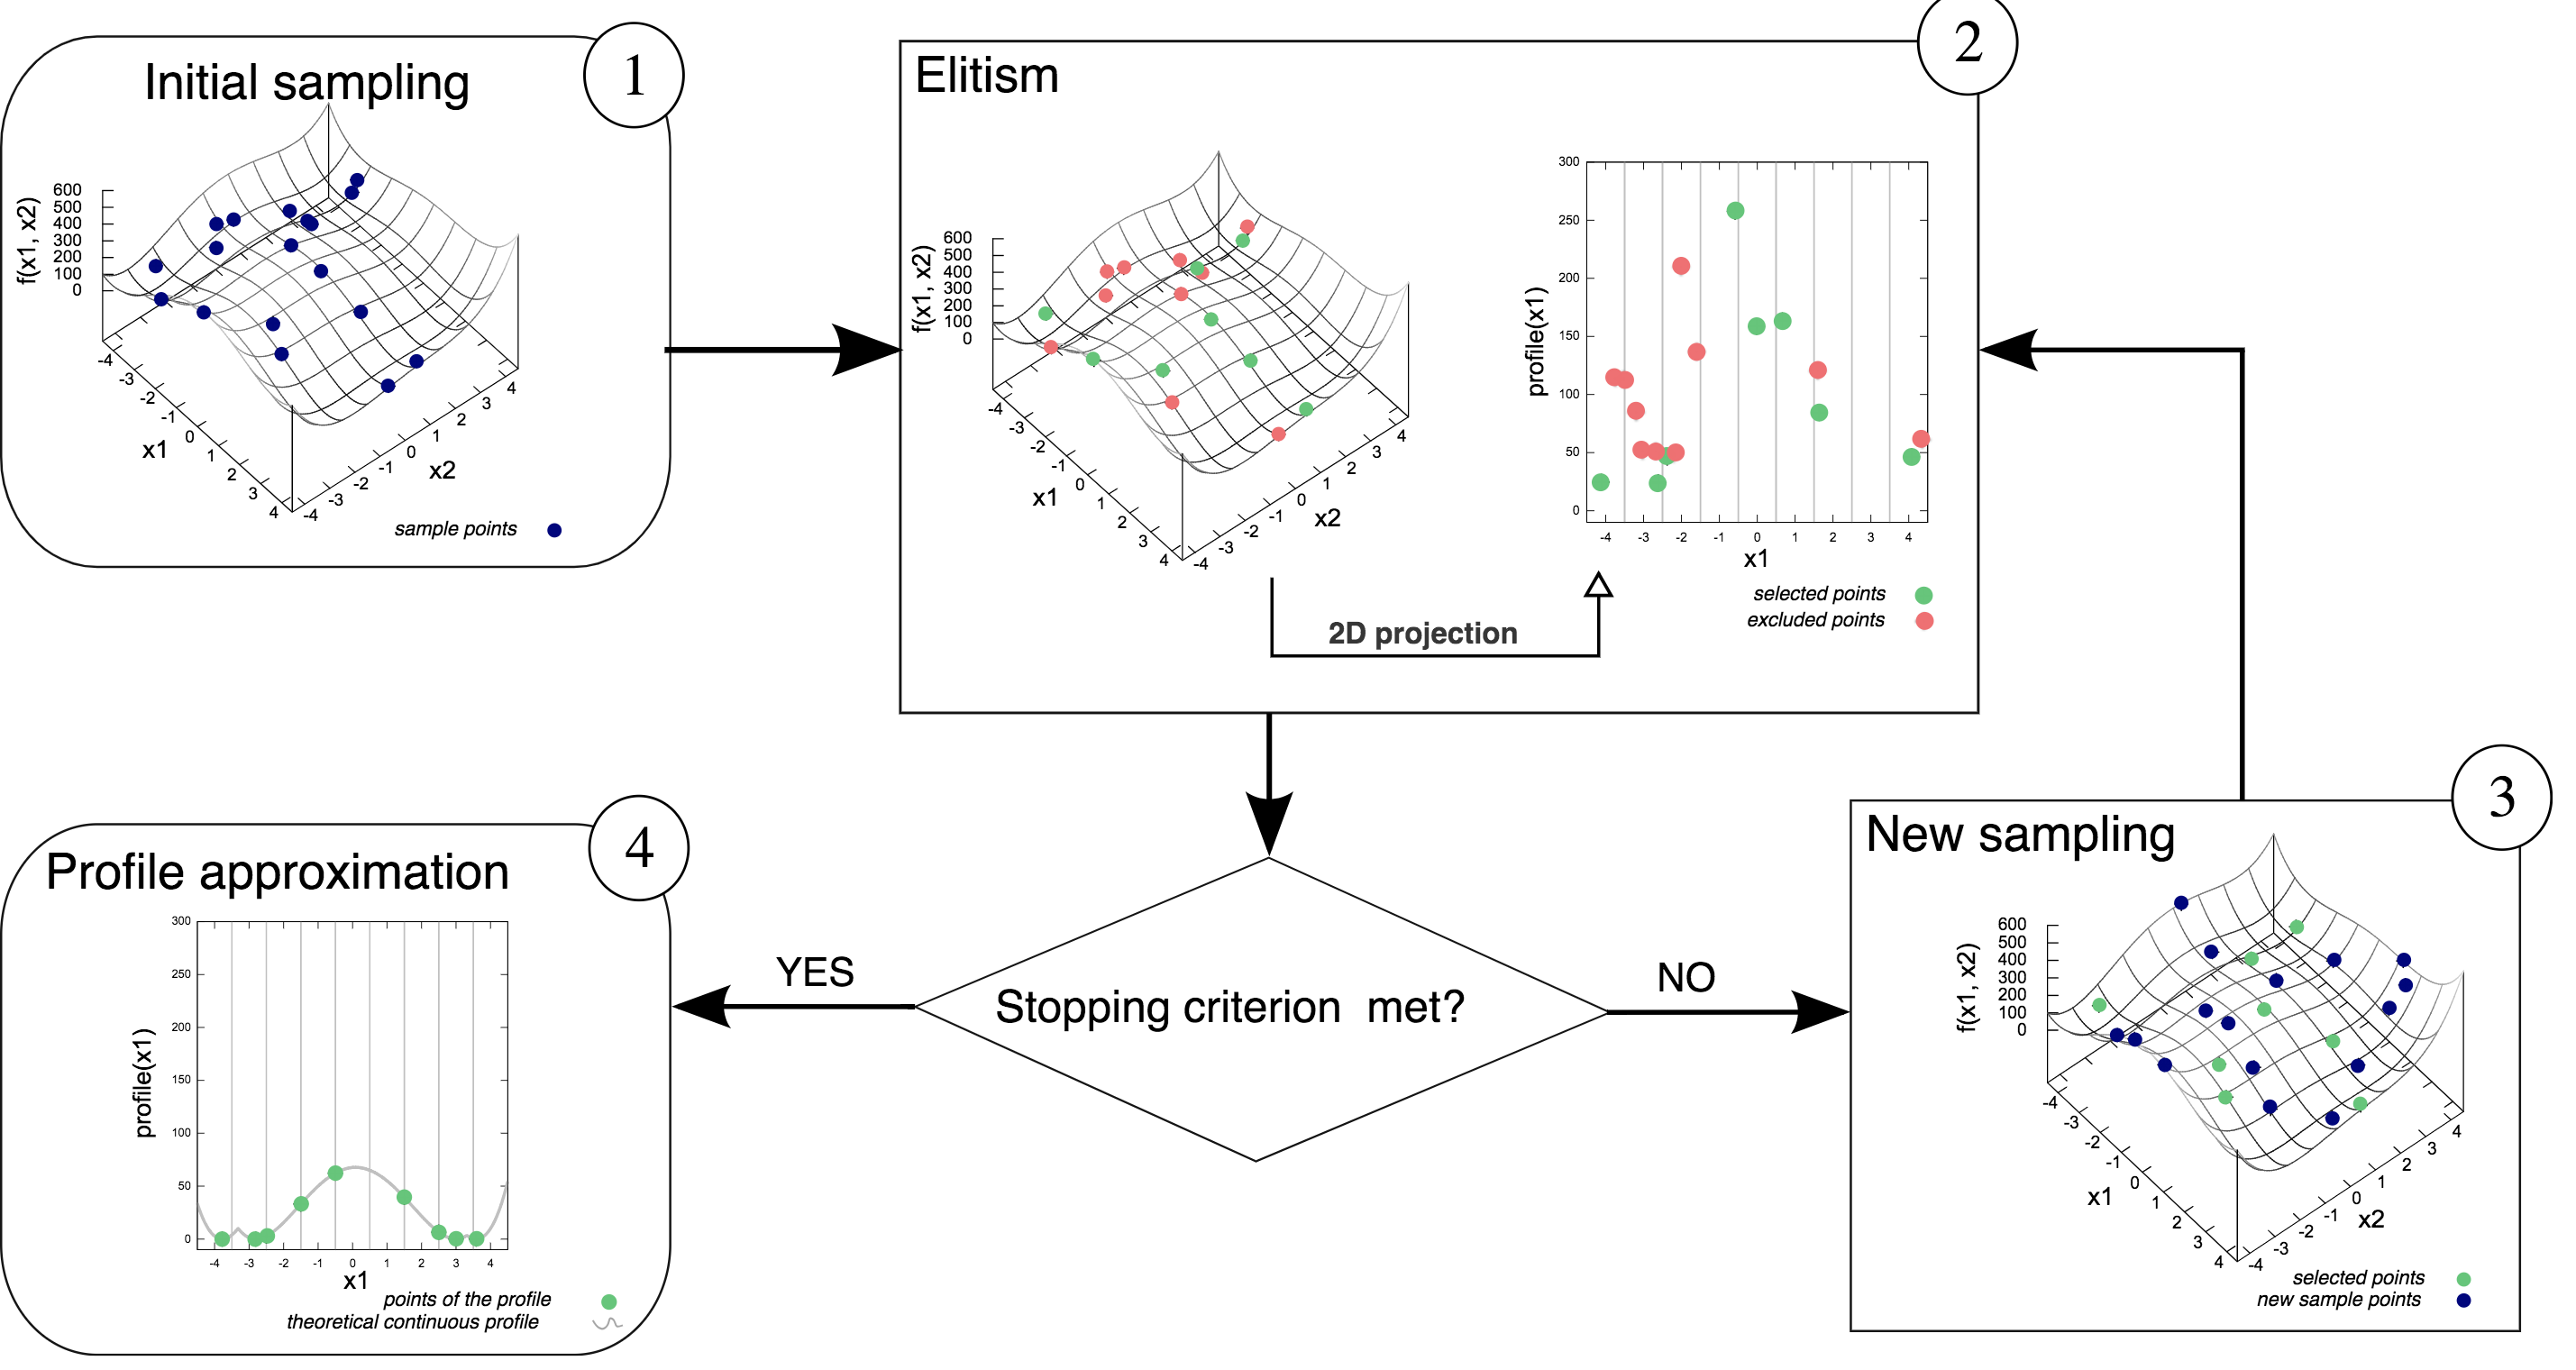
\includegraphics[width=\textwidth]{../20230629_IGN_BigData/figures/profil_algo.png}
}
	
%The profile algorithm
%
\medskip
\textit{Compute the best of calibration for hundreds of values along the definition domain of a parameter.}


%The method is tractable (even for ABMs):
%Converges almost as fast a single calibration.
%Handles stochasticity: 100x gain.
%Support for distributed computing: 1000x gain.	
	
}



\sframe{Profile algorithm}{
\centering
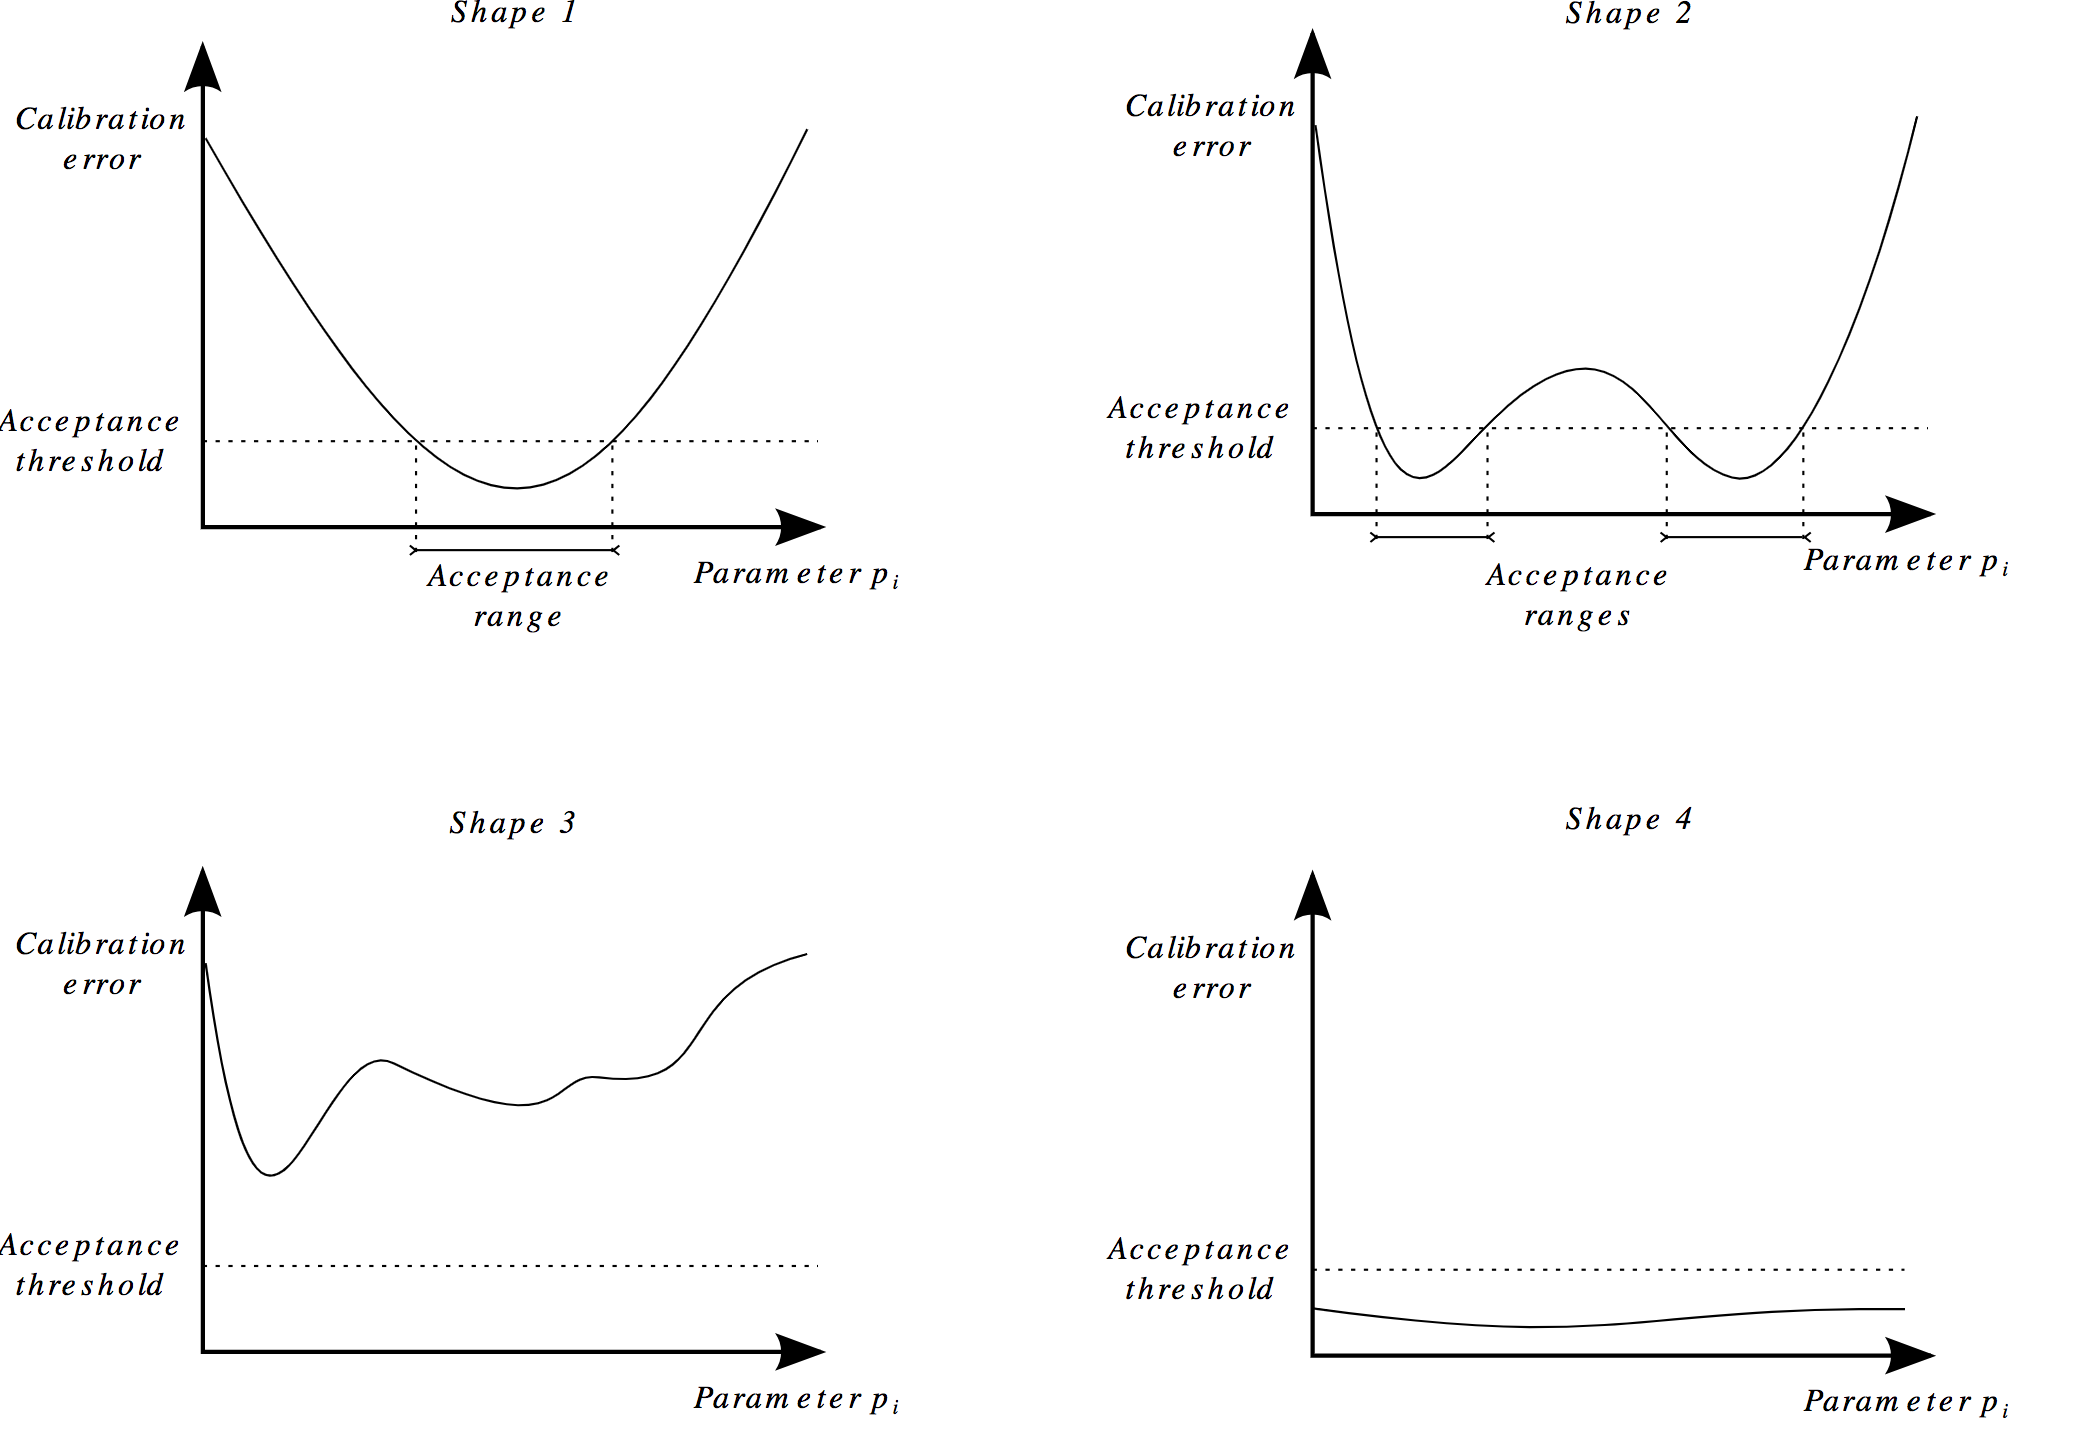
\includegraphics[width=\textwidth]{../20230629_IGN_BigData/figures/profil_interpretation.png}
}


\sframe{Results}{

	\centering
	
	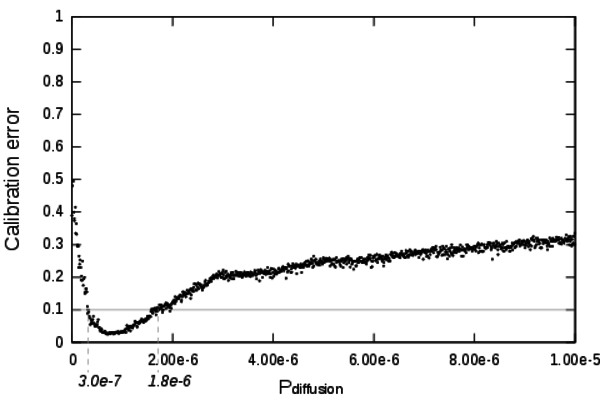
\includegraphics[width=\textwidth]{../20230629_IGN_BigData/figures/PdiffusionZ.png}

}

\sframe{Results}{

	\centering
	
	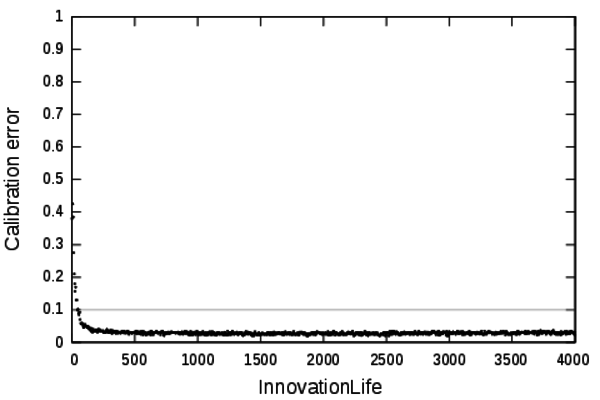
\includegraphics[width=\textwidth]{../20230629_IGN_BigData/figures/InnovationLife.png}

%Conclusion
%How to assess:

%the sufficiency of the mechanisms Y
%the necessity of the mechanisms Y
%the uniqueness of the mechanisms ?

}


\sframe{Unicity \cite{cottineau2014evolution}}{

%

\textit{Automate the confrontation of alternative hypothesis / mechanisms.}

\medskip

\centering
	
	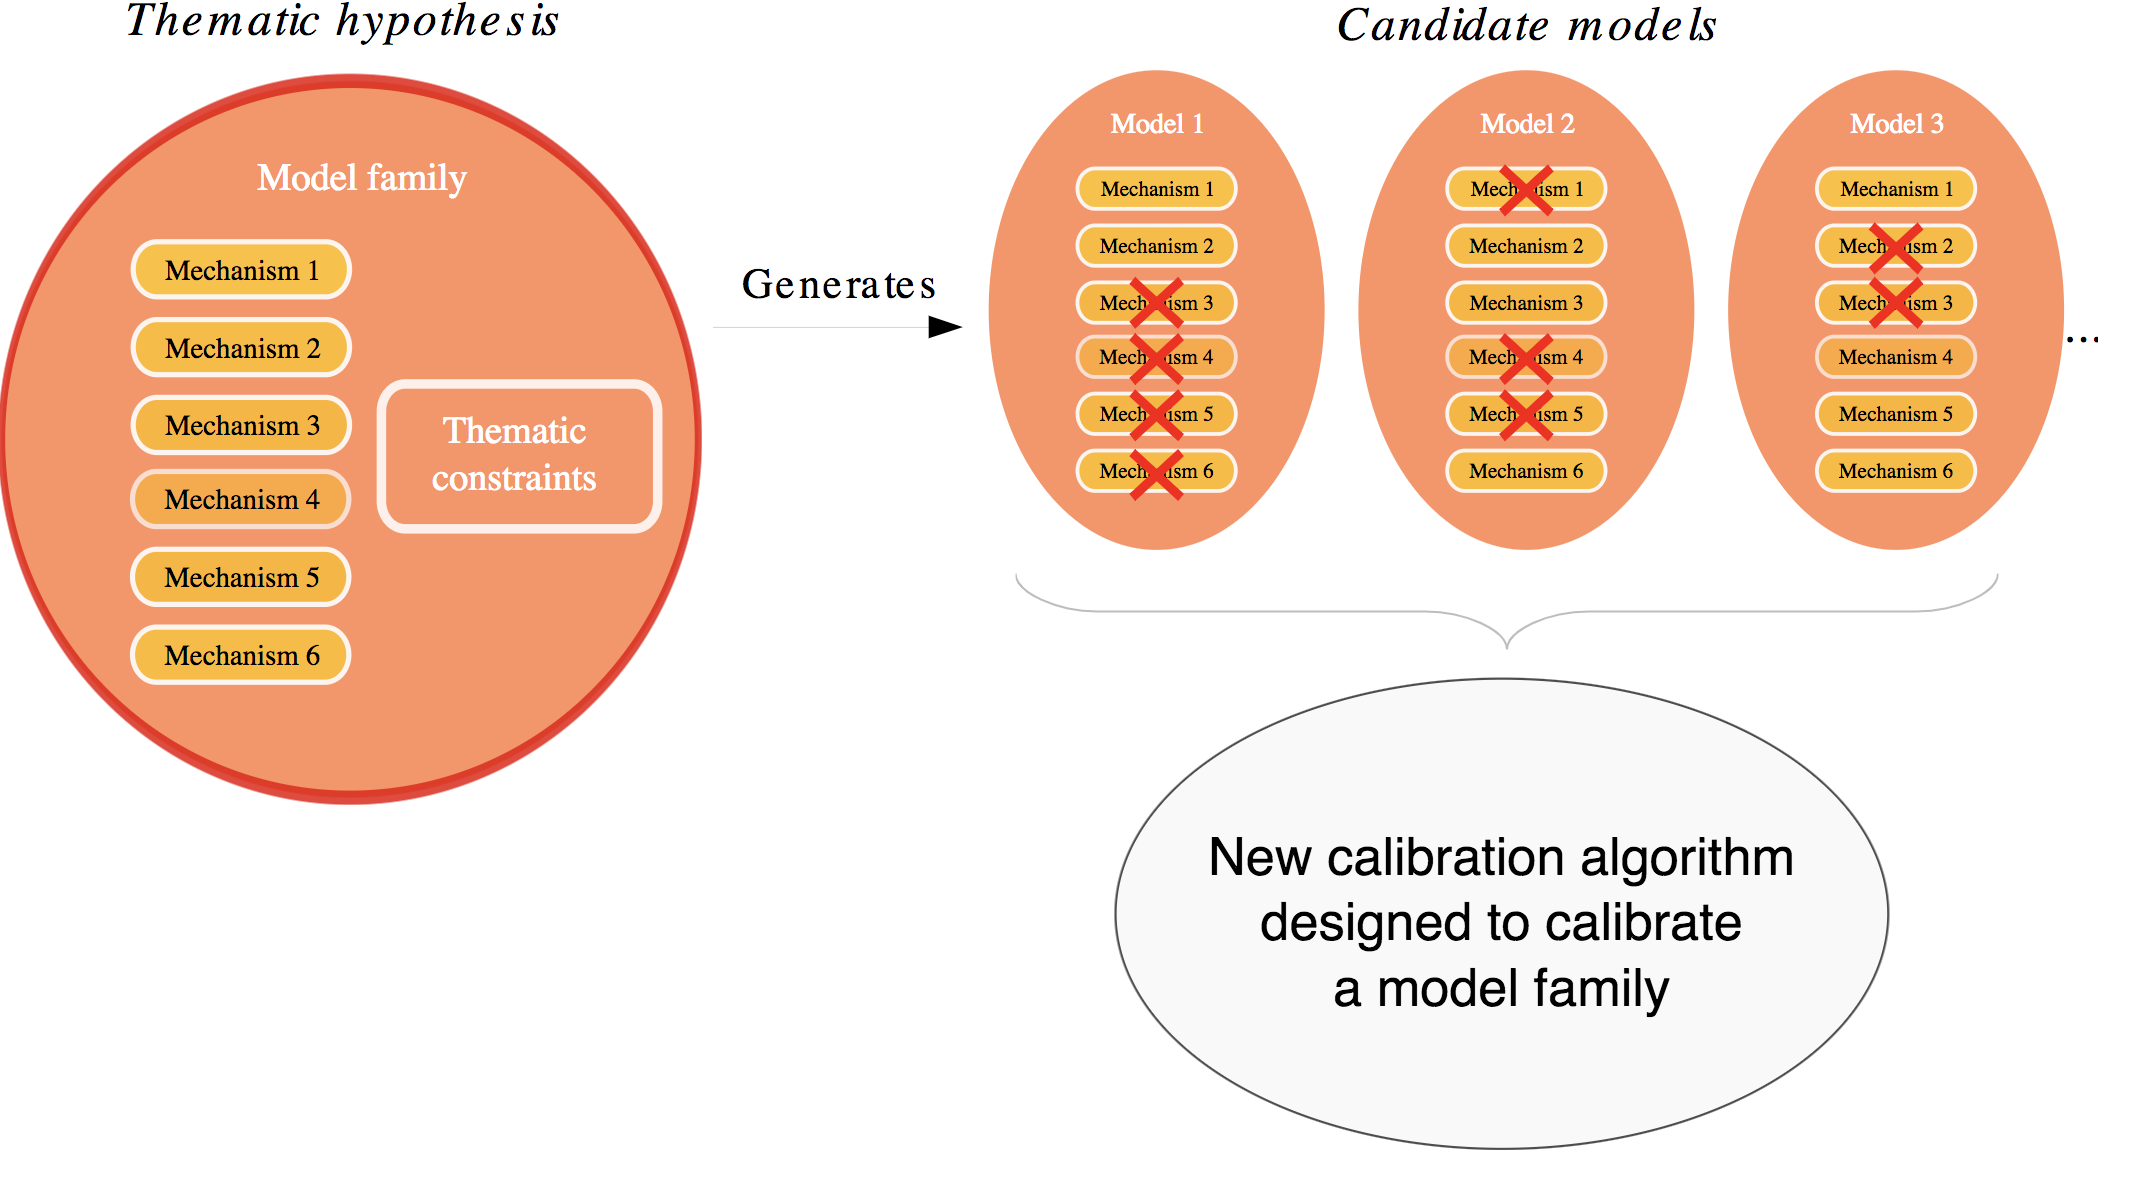
\includegraphics[width=\textwidth]{../20230629_IGN_BigData/figures/simfamily.png}

}


\sframe{Objective}{


%What we are running after?

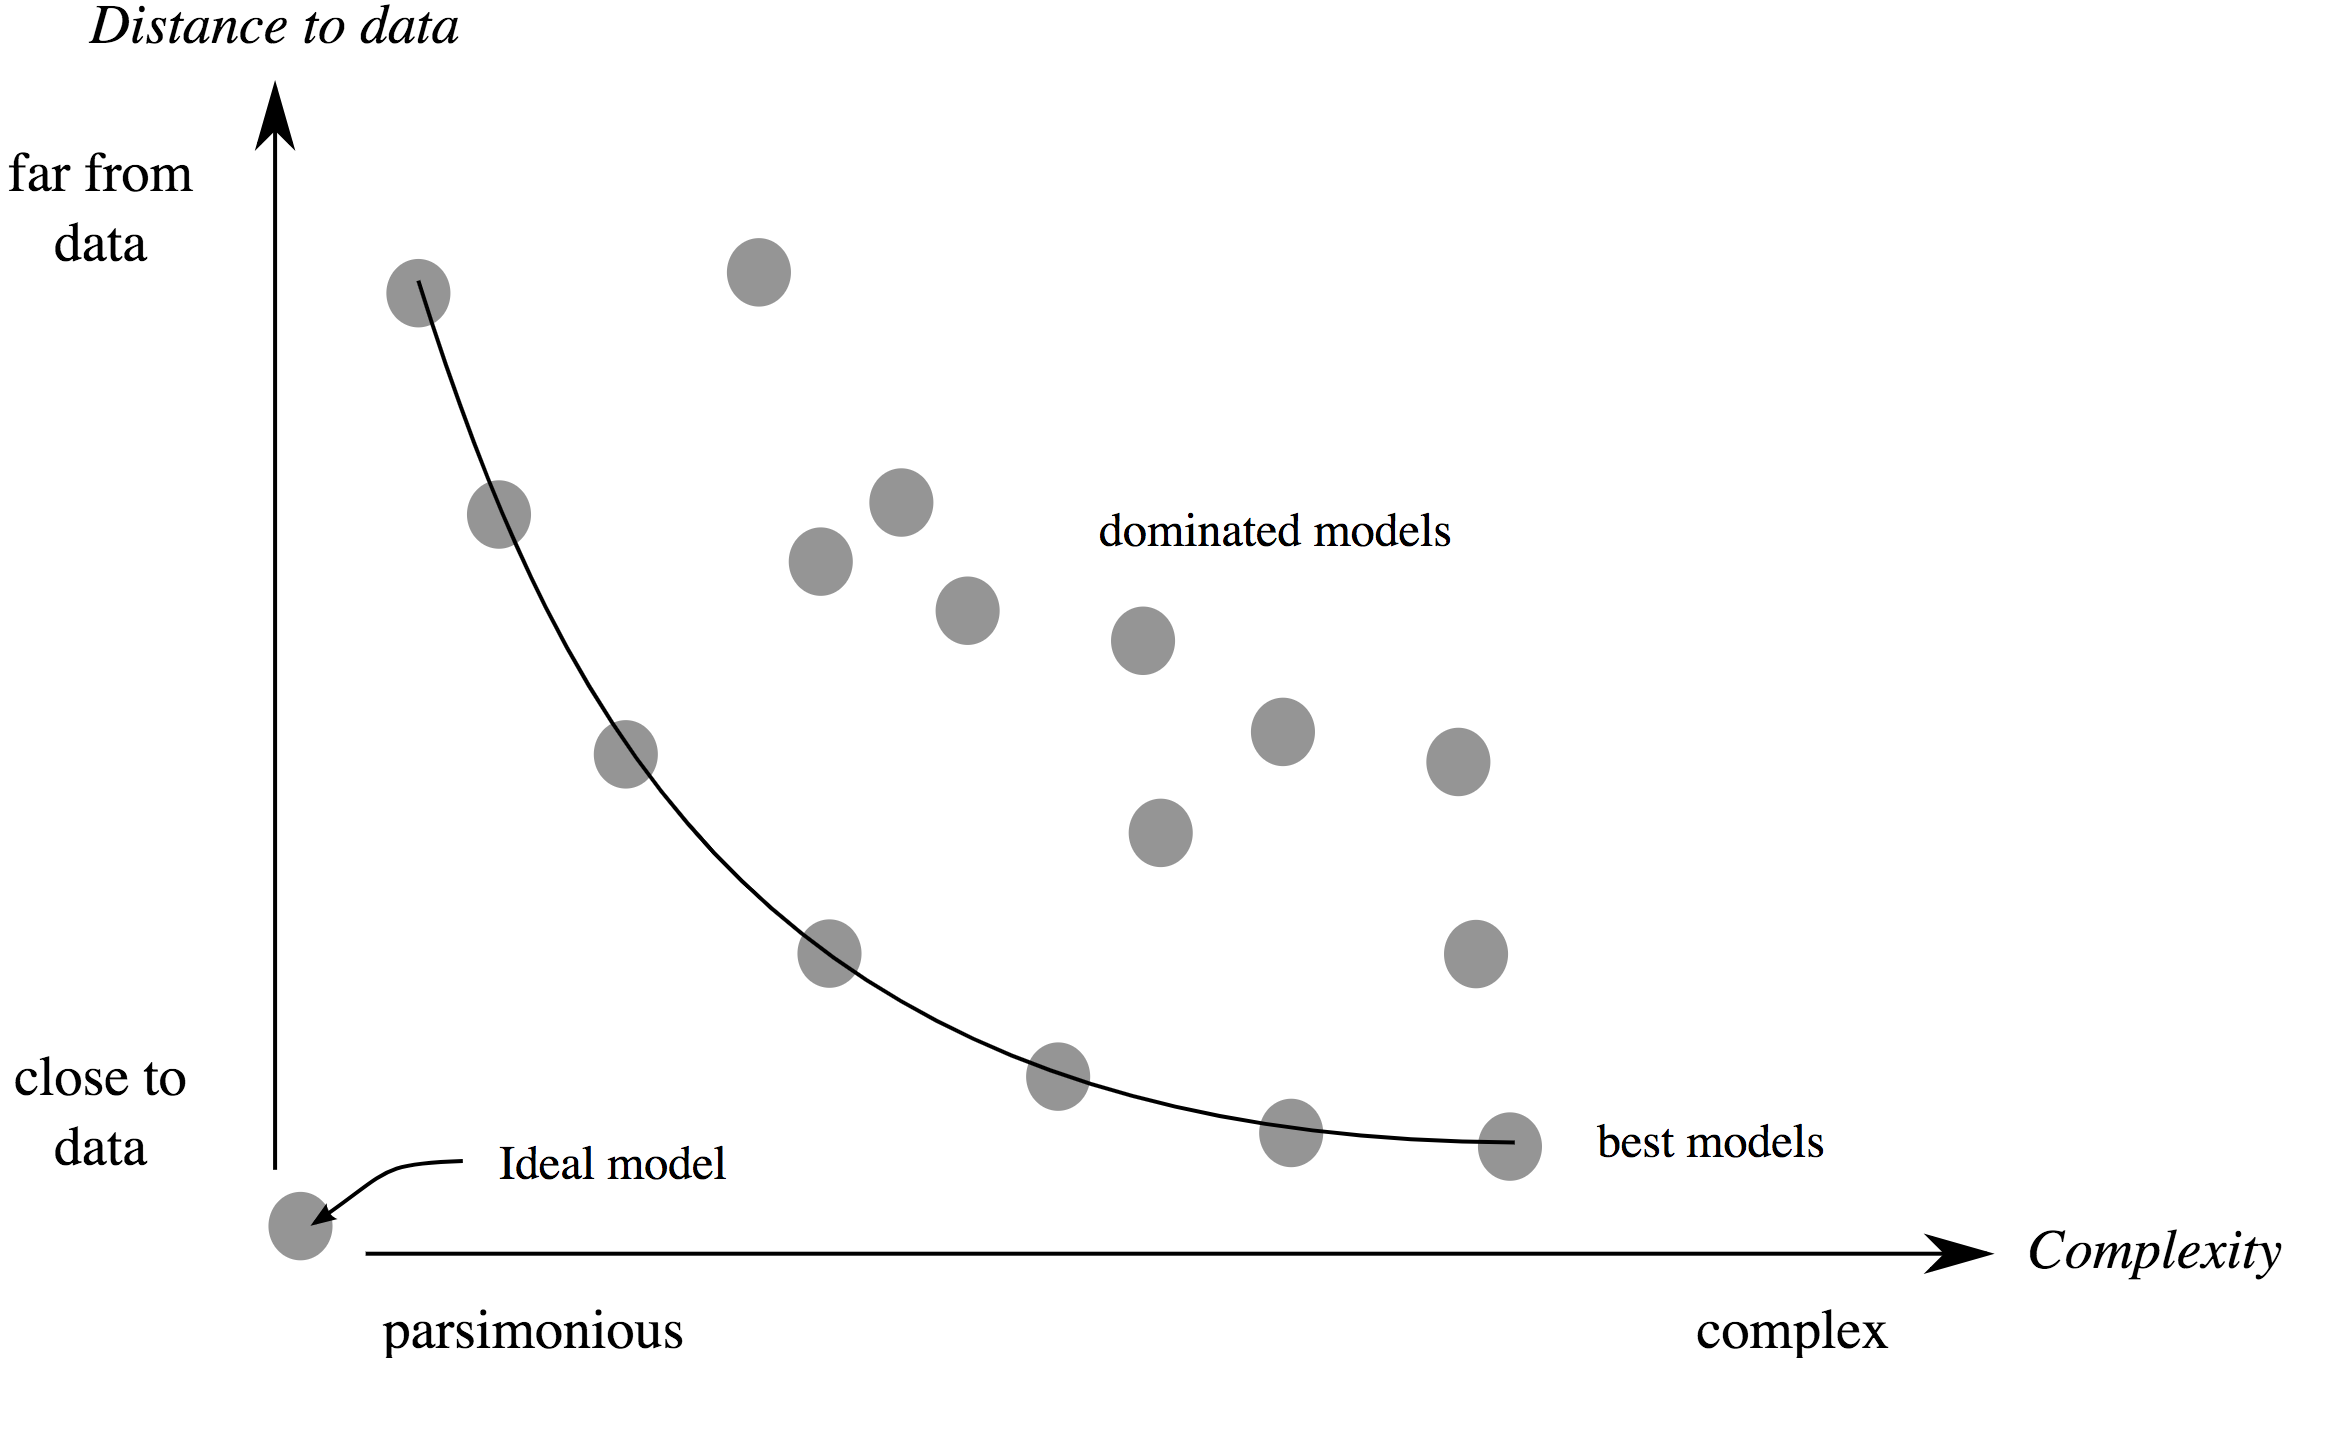
\includegraphics[width=\textwidth]{../20230629_IGN_BigData/figures/paretocomplexityfit.png}

}

\sframe{Multi-modeling (64 models)}{

%64 models

\centering

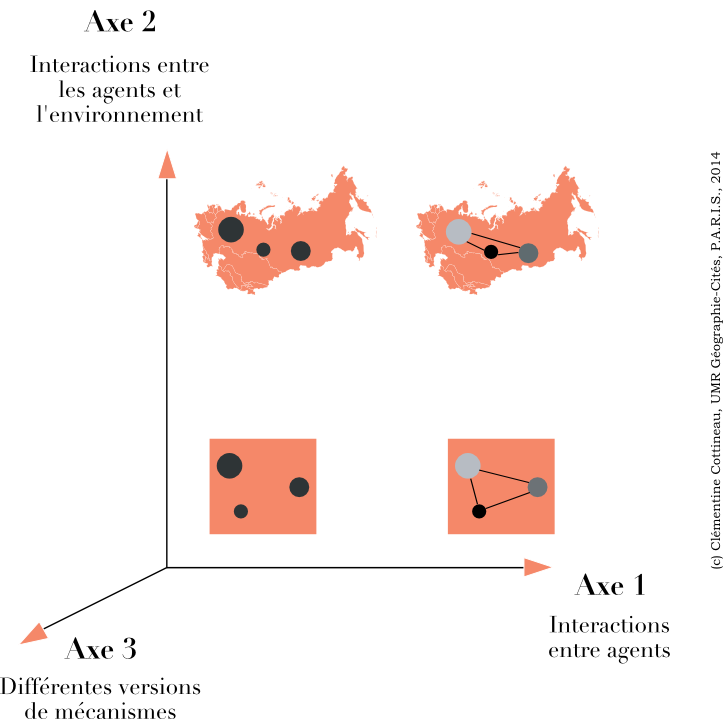
\includegraphics[width=0.8\textwidth]{../20230629_IGN_BigData/figures/marius_complexification.png}

}



\sframe{Calibration of the model family}{

%
\textit{Compute the best set of parameters for all 64 models, using a niched NSGA2 algorithm.}

\bigskip

\centering

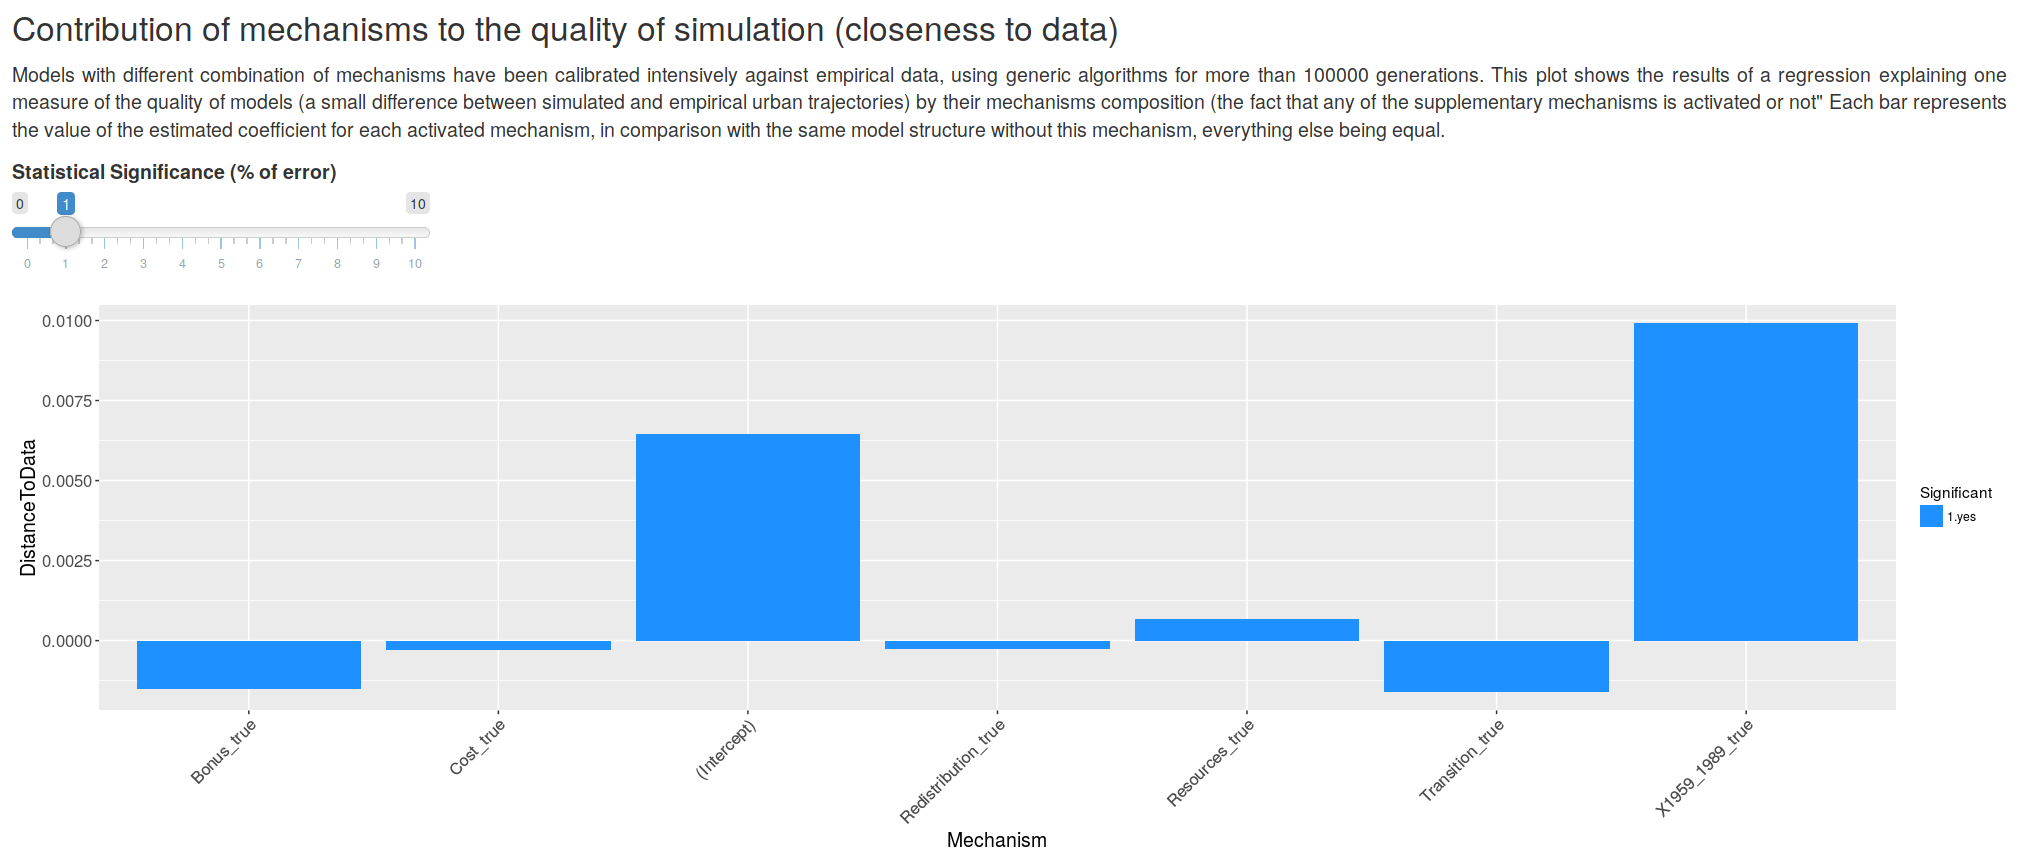
\includegraphics[width=\textwidth]{../20230629_IGN_BigData/figures/varius_big.png}


}





\sframe{Novelty search \cite{10.1371/journal.pone.0138212}}{

\centering

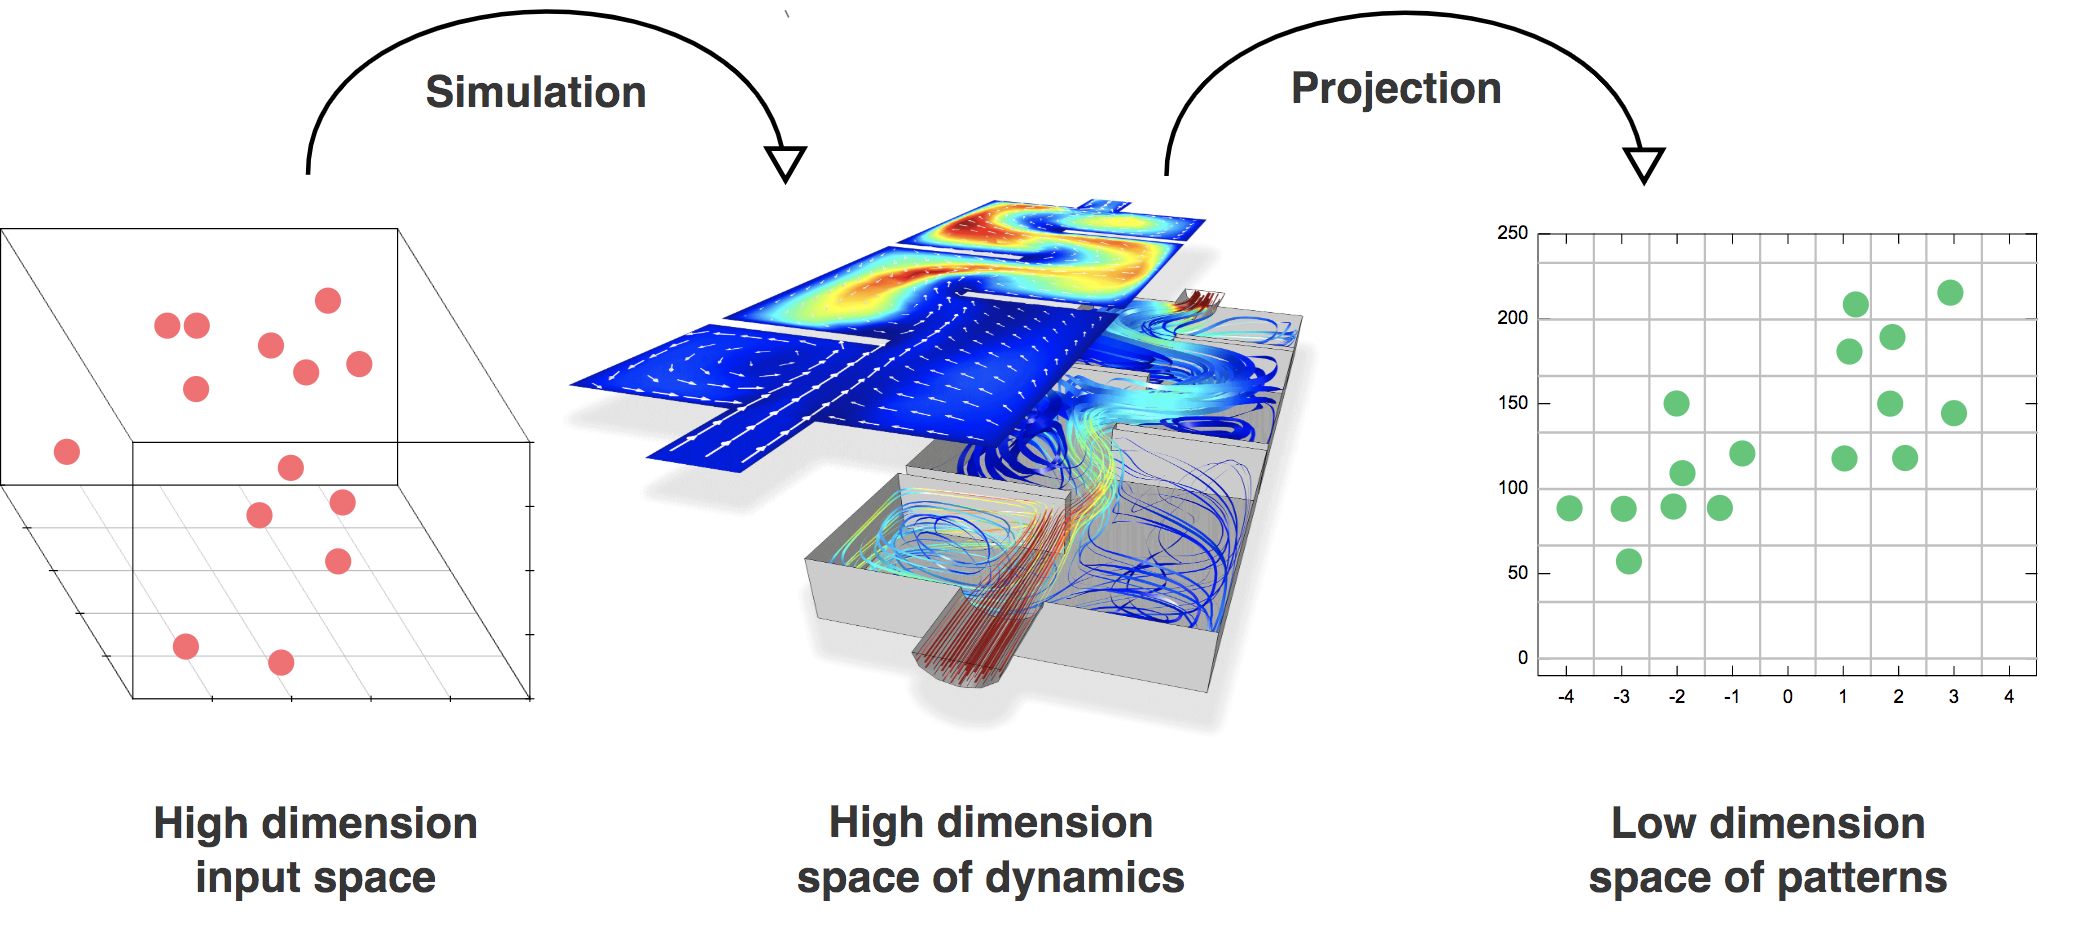
\includegraphics[width=\textwidth]{../20230629_IGN_BigData/figures/pse_algo.png}

}

\sframe{Novelty search}{

%

\textit{The inputs producing rare patterns have high fitness values.}

\centering

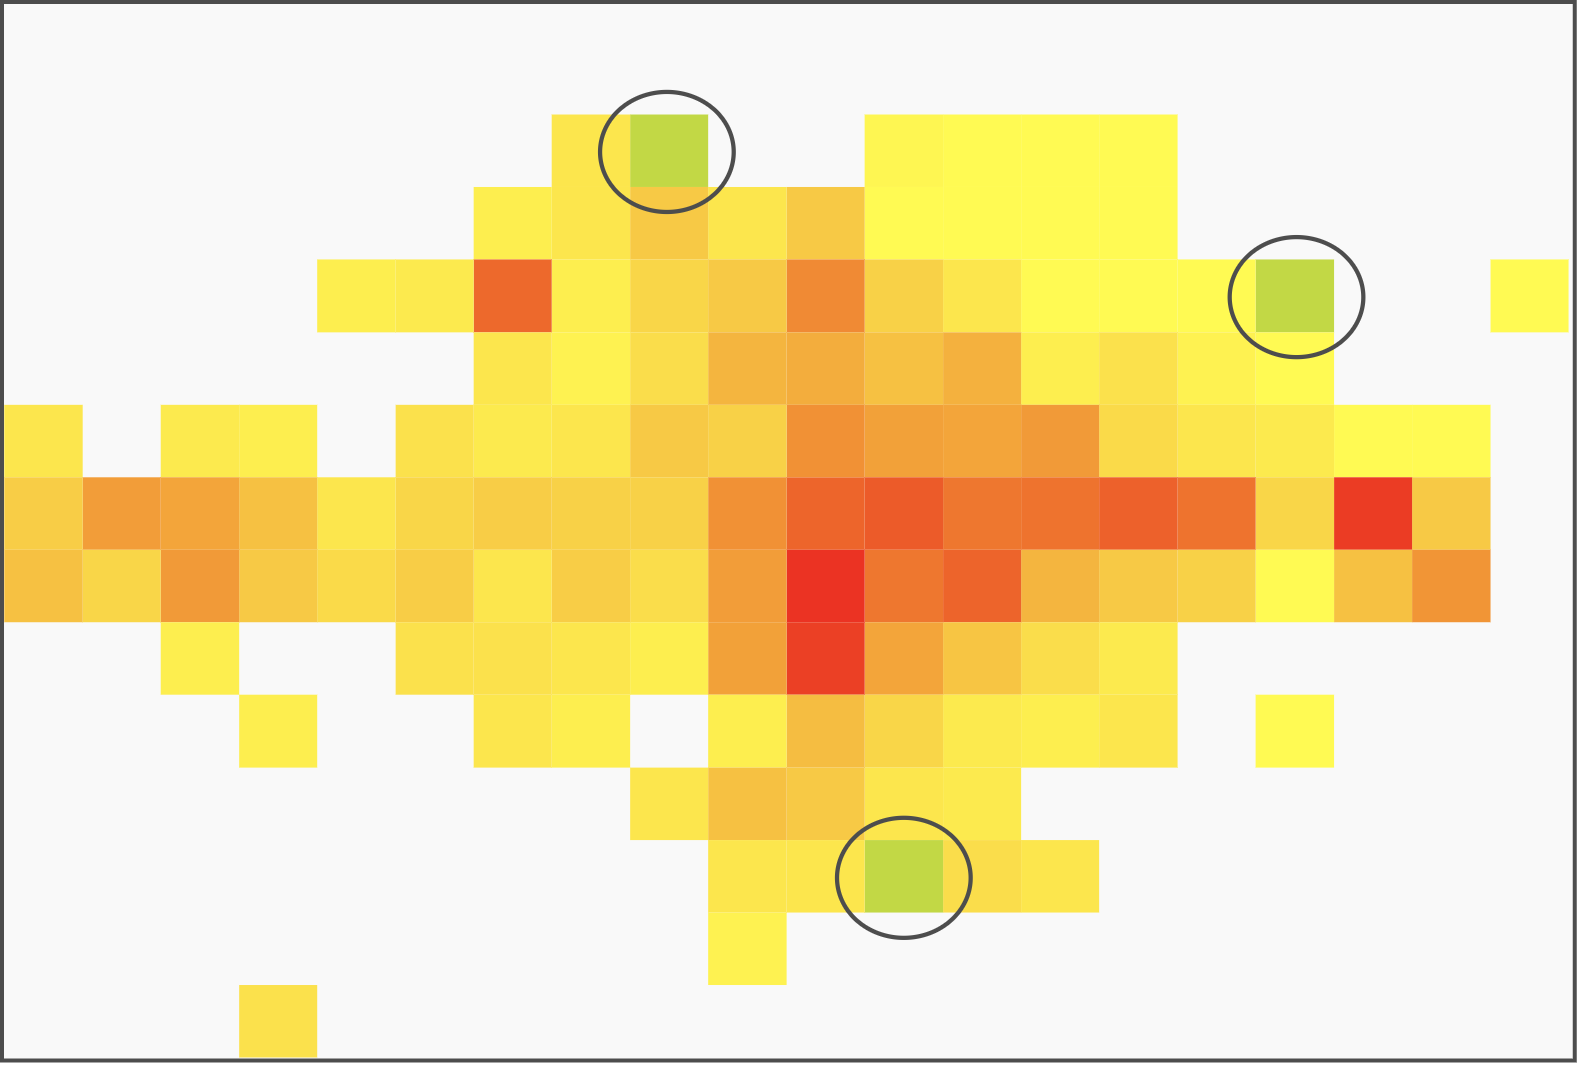
\includegraphics[width=0.9\textwidth]{../20230629_IGN_BigData/figures/hitmap.png}

}


\sframe{Results}{

\centering

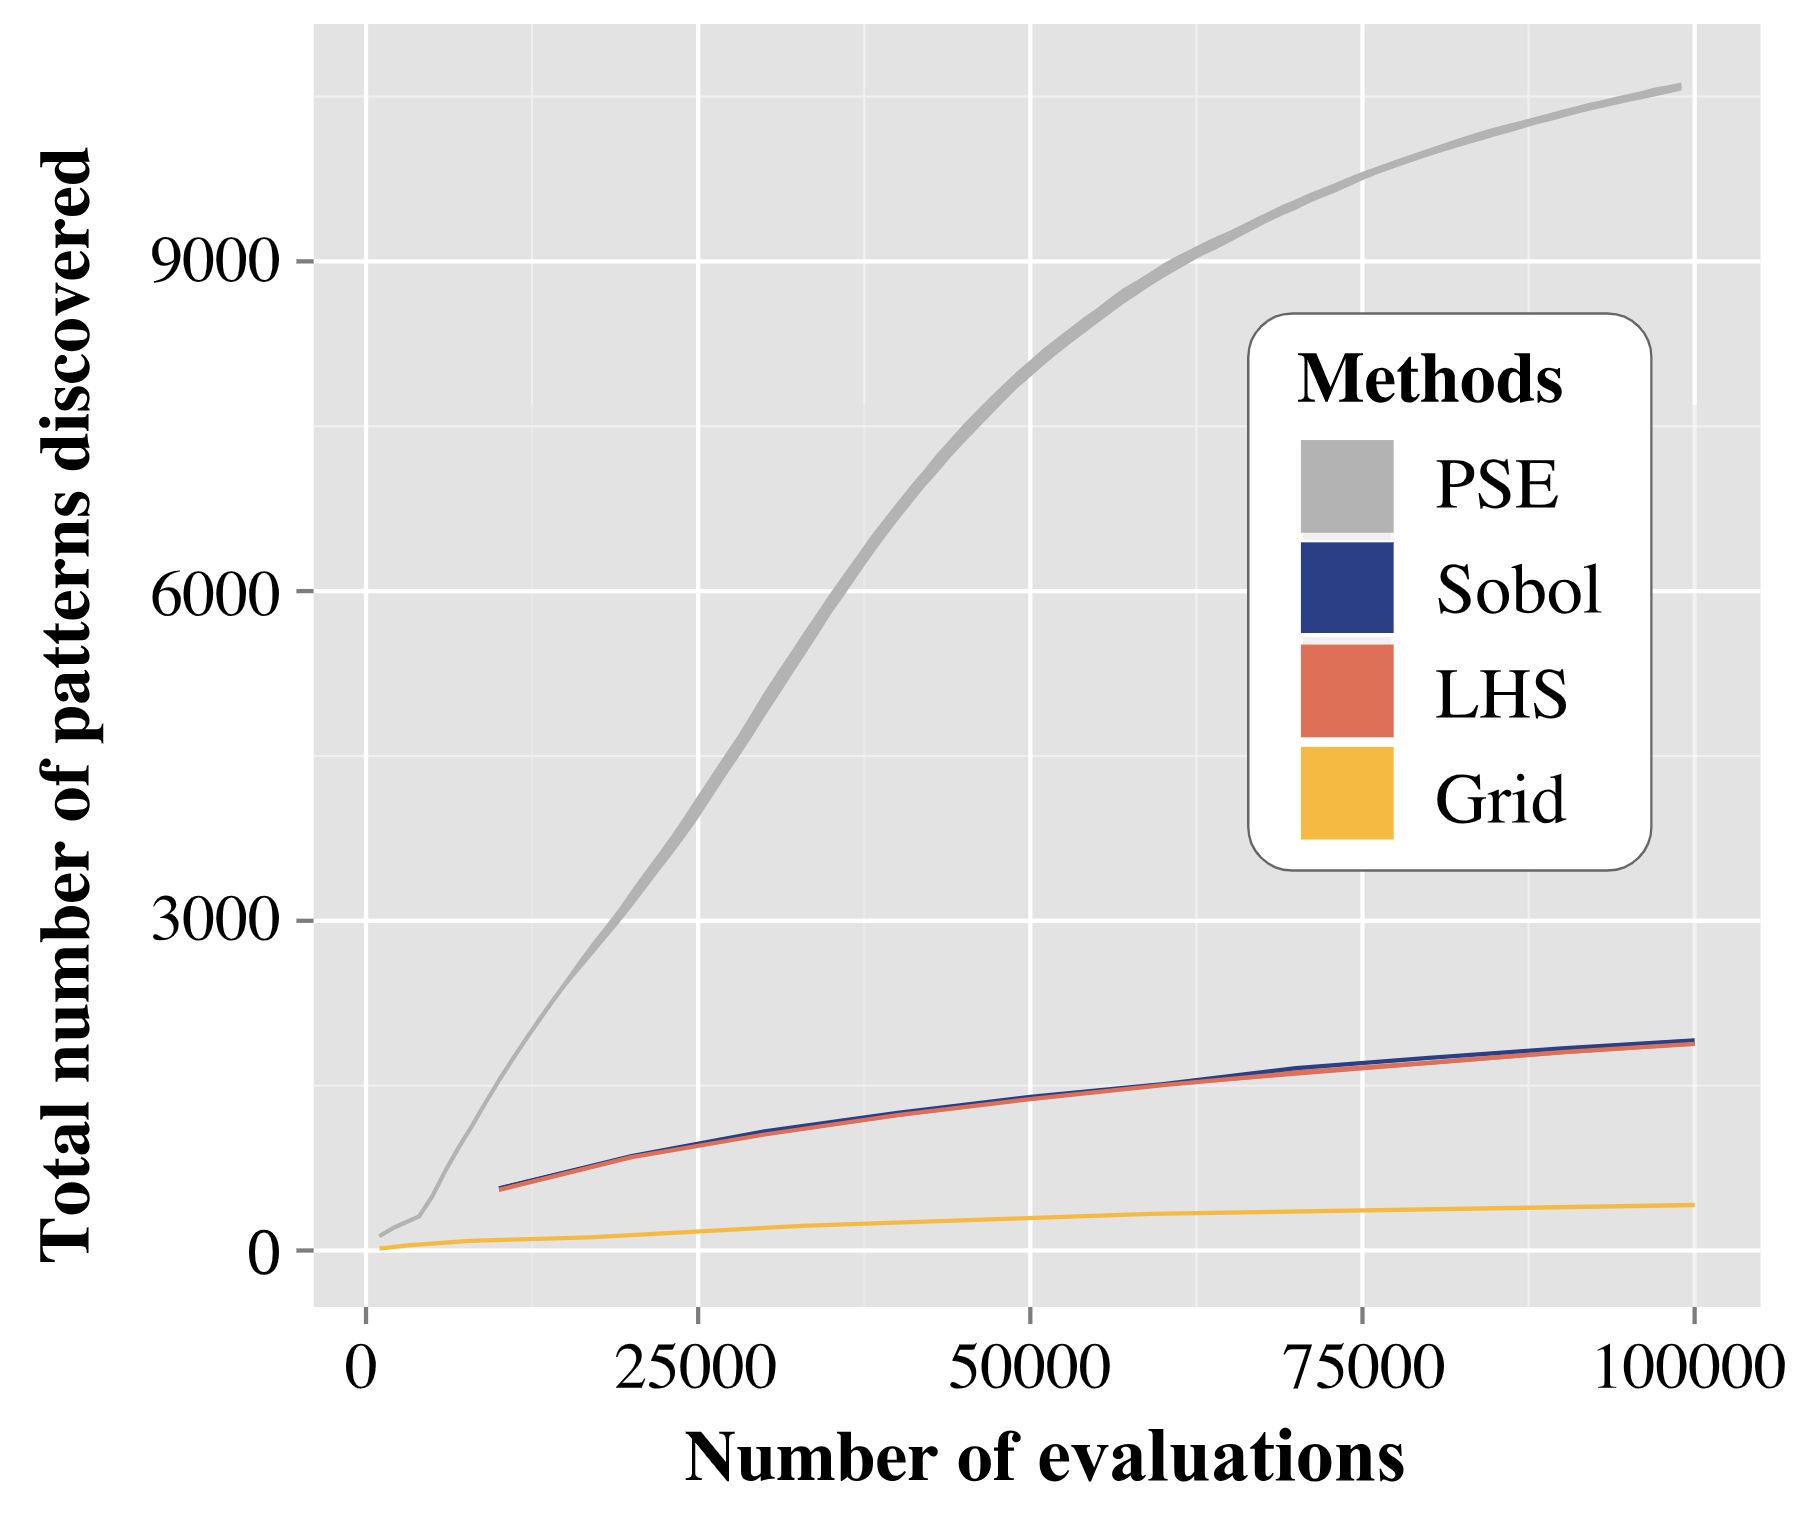
\includegraphics[width=0.9\textwidth]{../20230629_IGN_BigData/figures/flockingvolume.png}

}

\sframe{Results}{

\centering

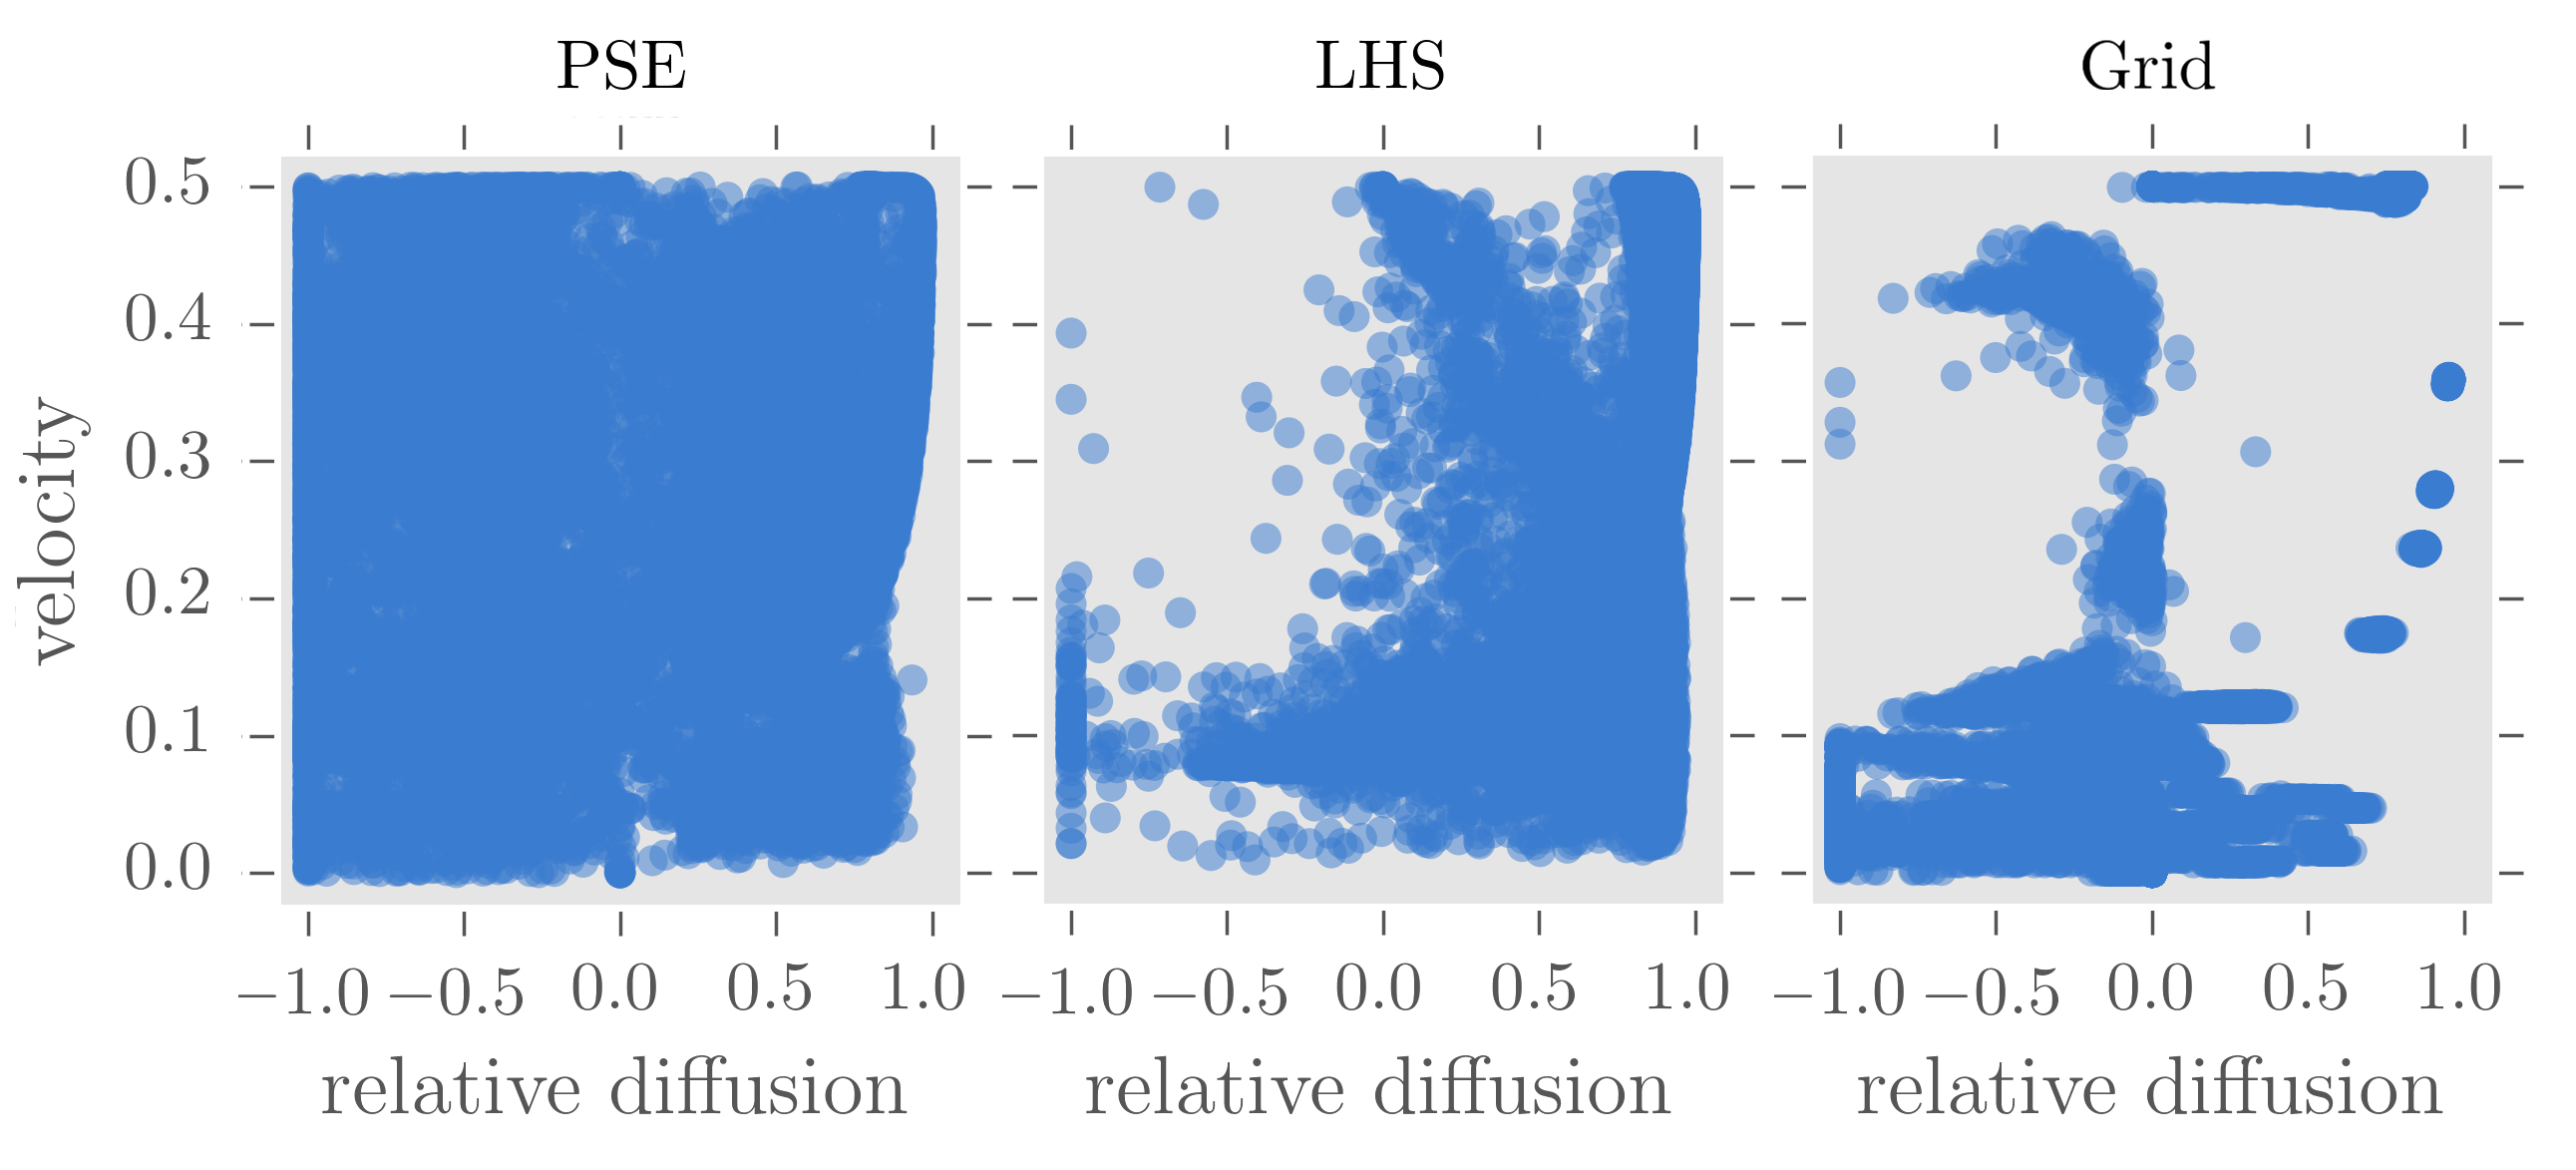
\includegraphics[width=\textwidth]{../20230629_IGN_BigData/figures/flockingpatterns.png}

}

\sframe{Results}{

\centering

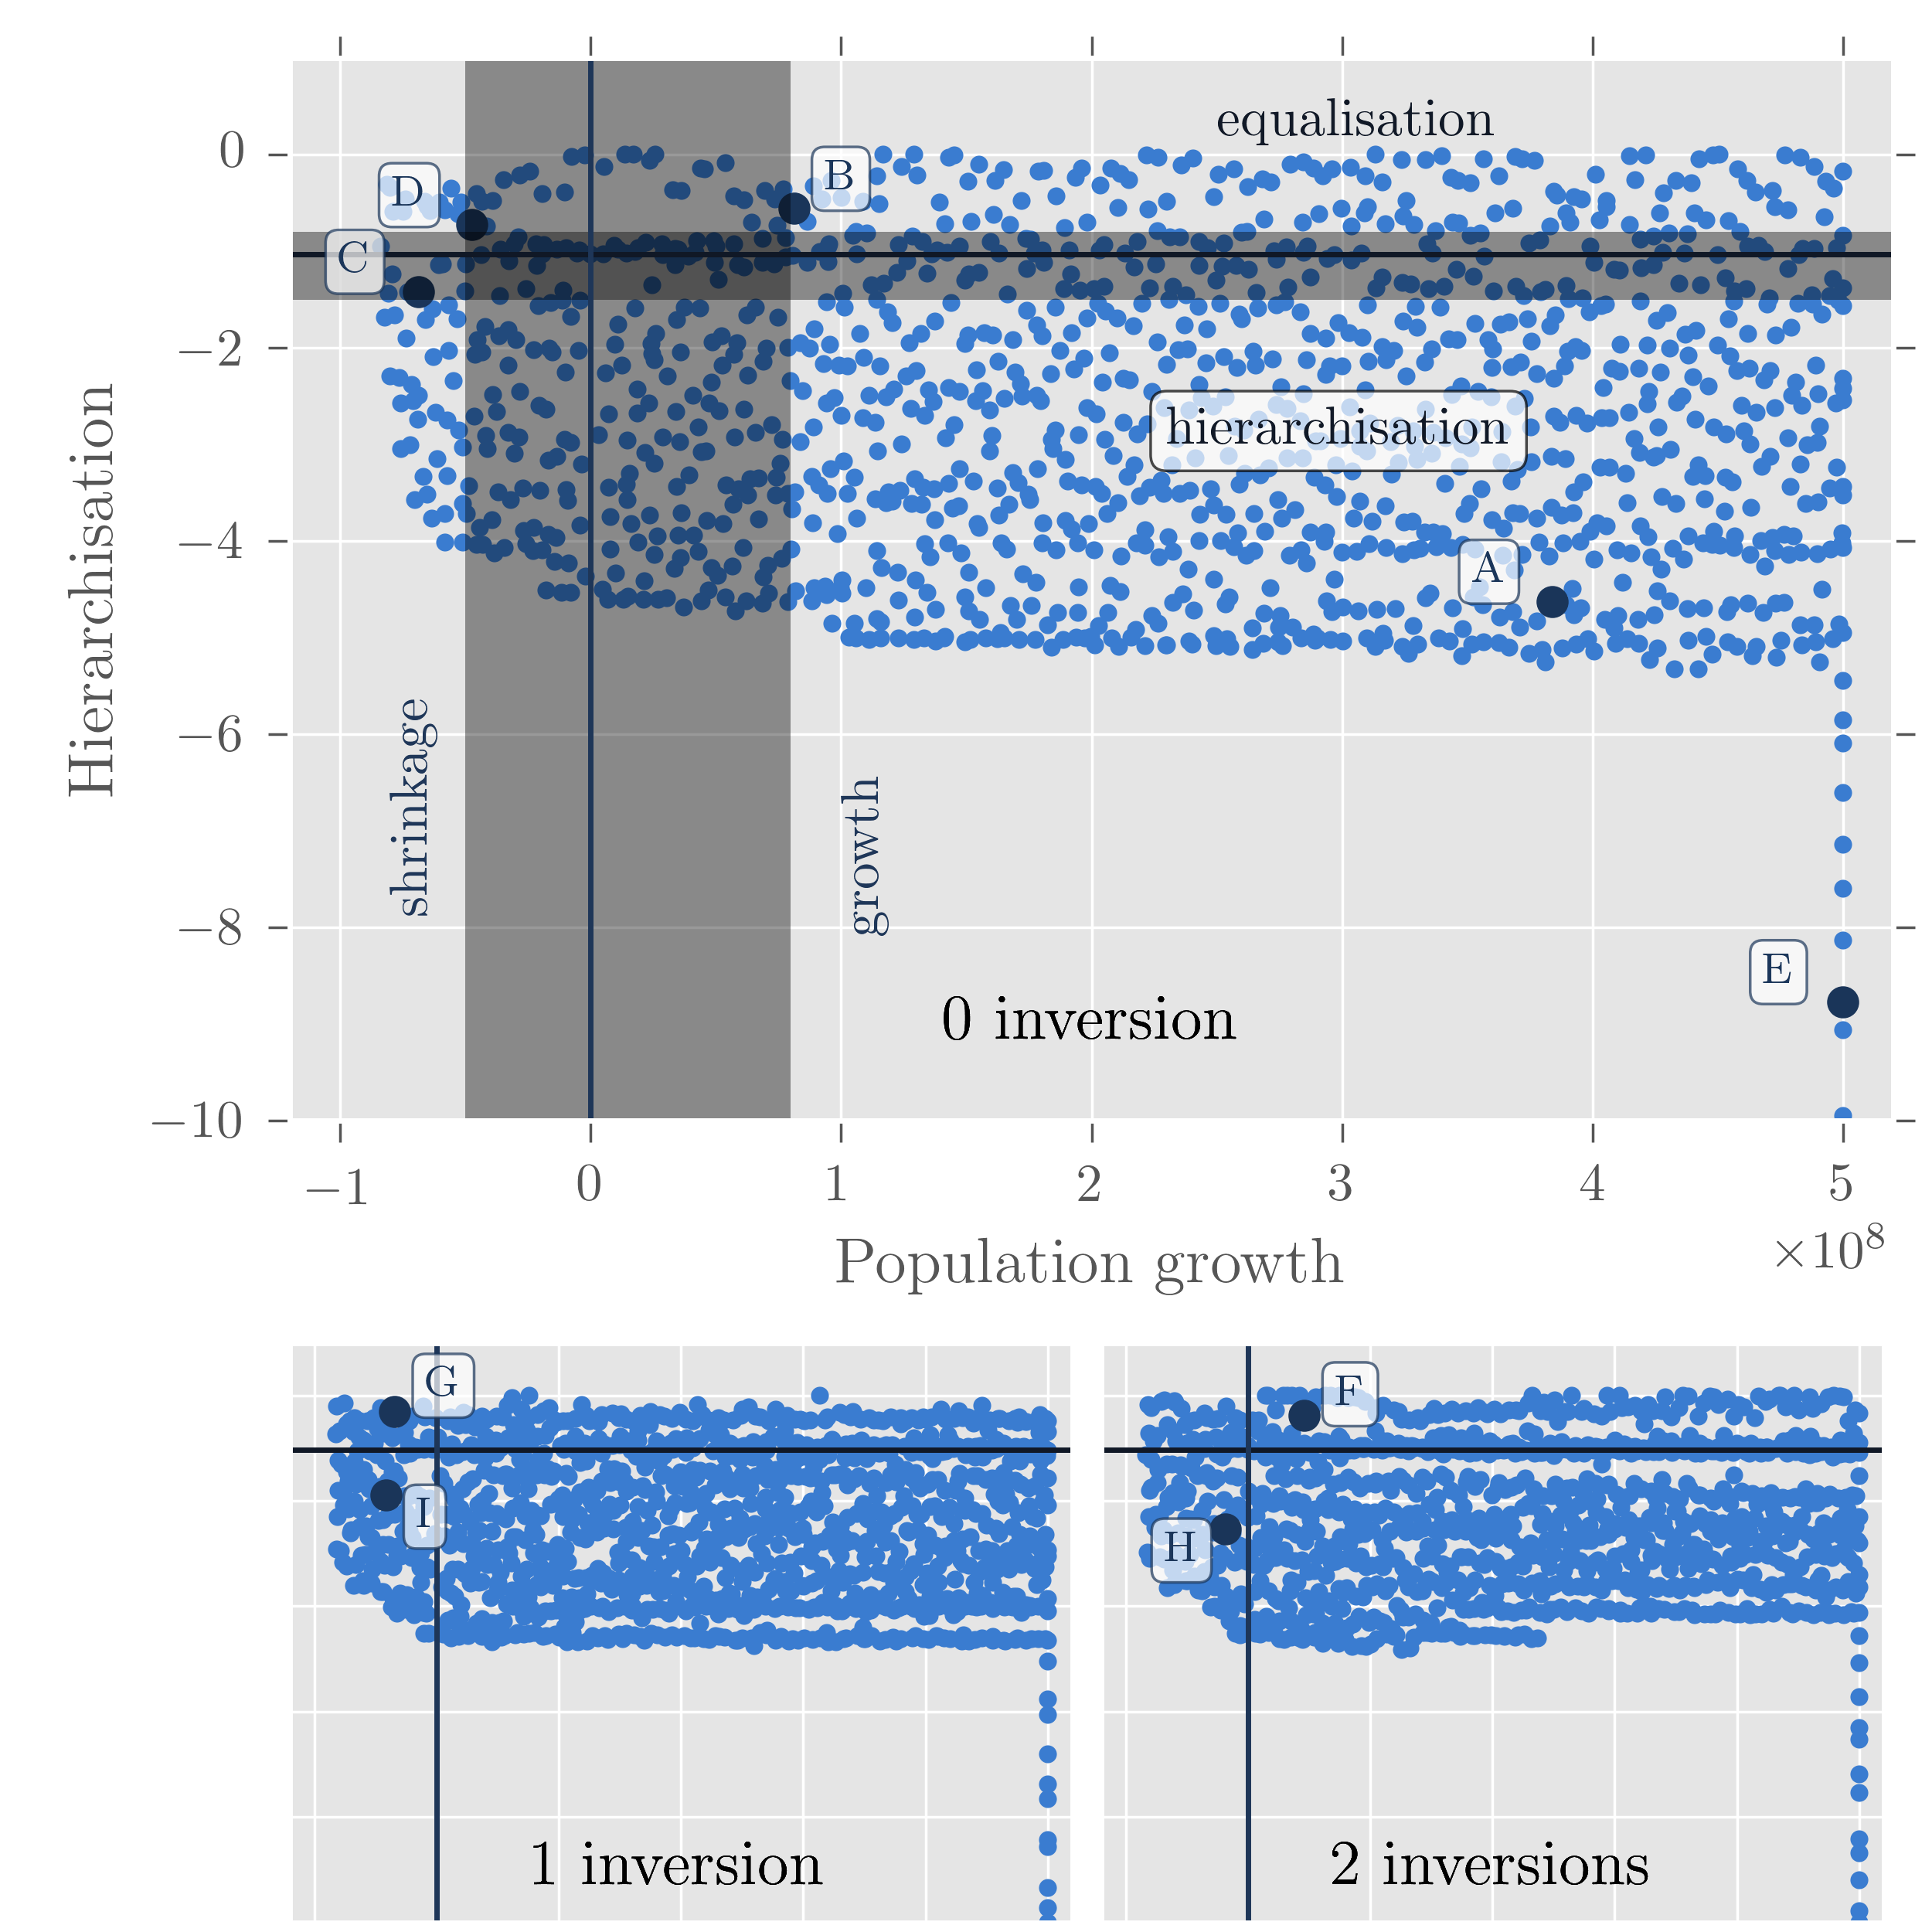
\includegraphics[width=0.6\textwidth]{../20230629_IGN_BigData/figures/pse_marius.png}

%Interpretation
%All expected/observed patterns are produced: the model is generic enough.
%
%
%Unexepected patterns are found:
%
%aberations: better constrain the model,
%predictions: test them.

% Exemple OpenMOLE + SimPLU (IGN) https://simplu.openmole.org/

}

\sframe{Inverse problem}{


\centering

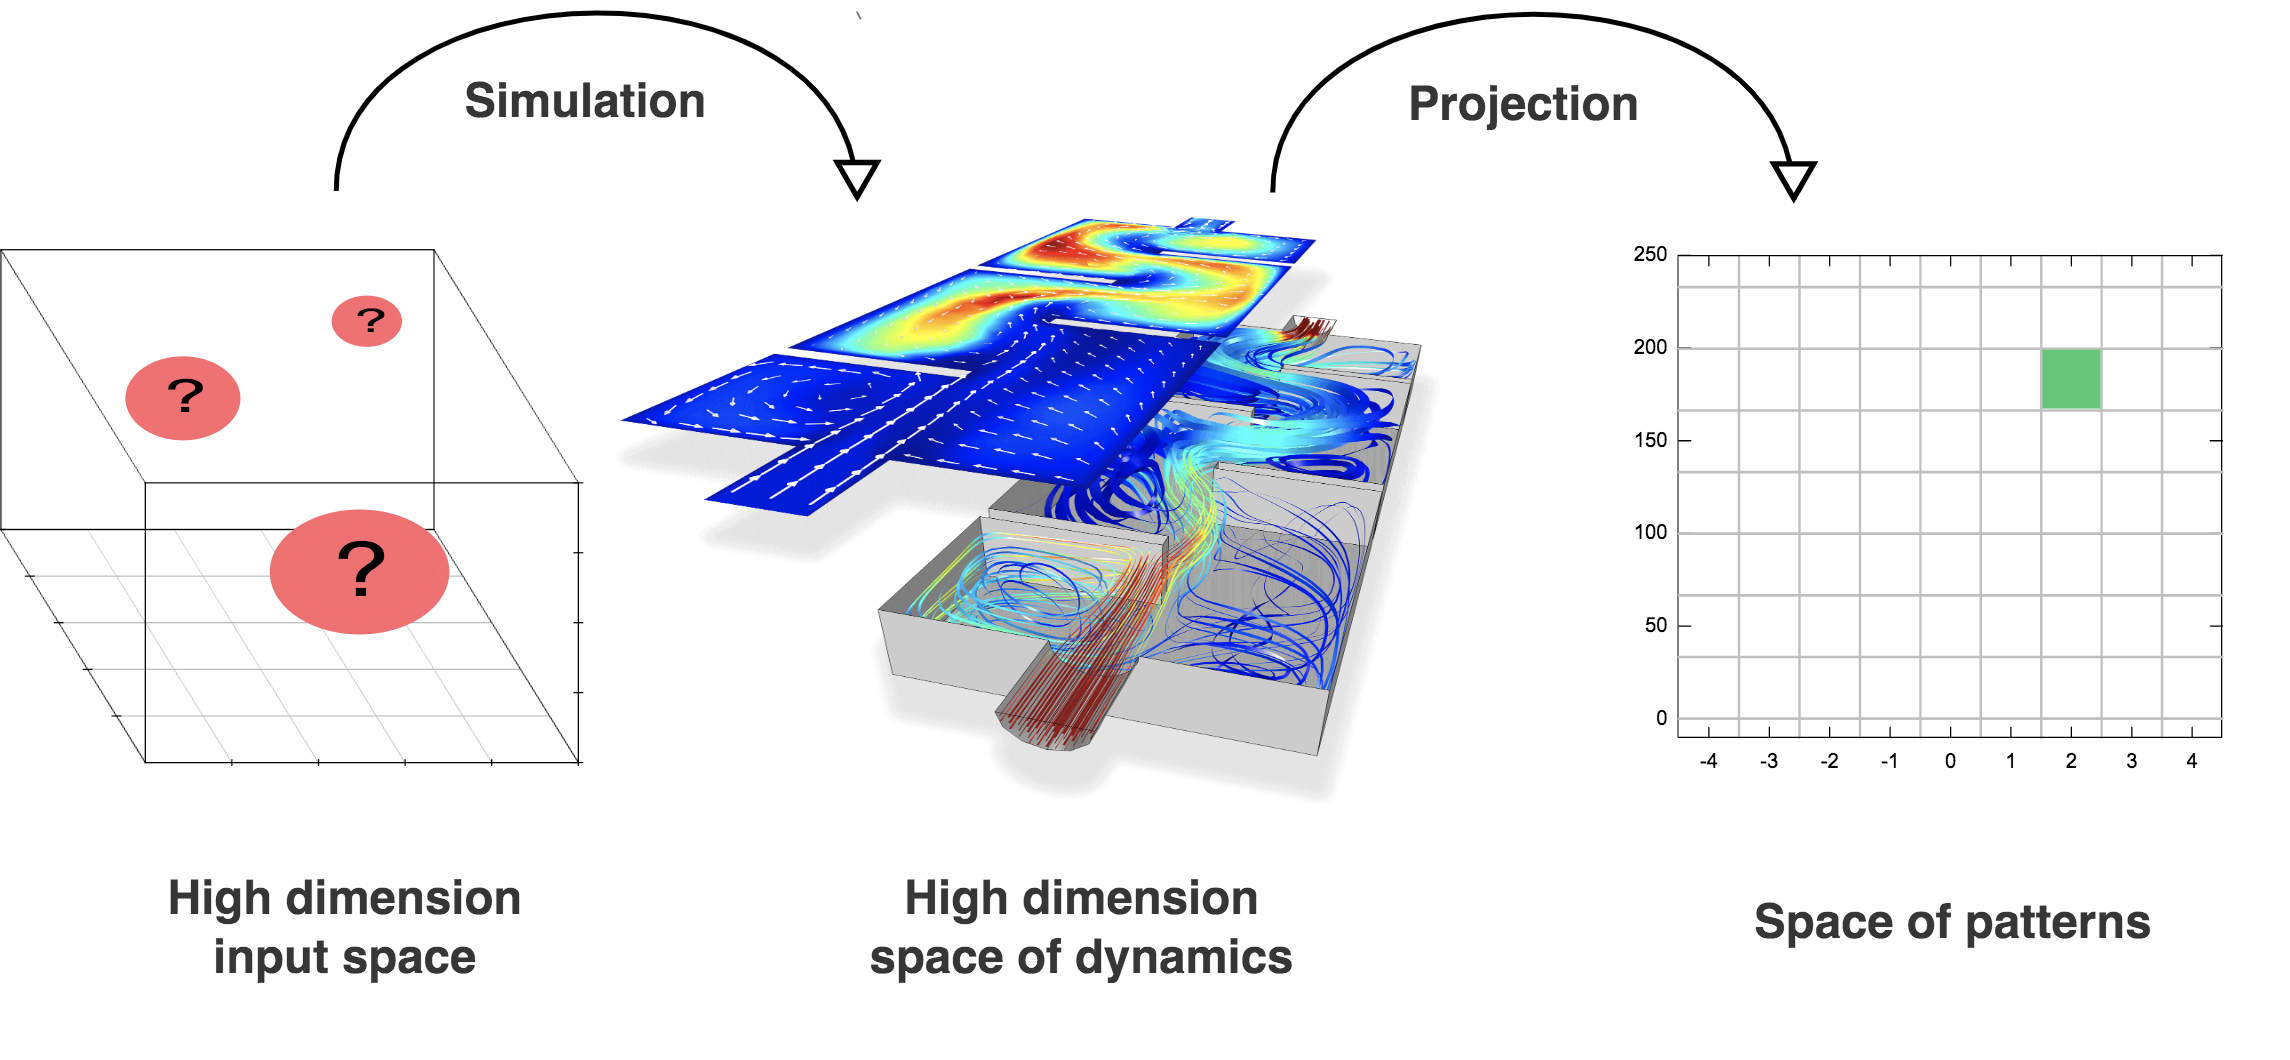
\includegraphics[width=\textwidth]{../20230629_IGN_BigData/figures/ose_algo.png}

}


\sframe{Results : minimising a Rastrigin function}{

$\Delta$ pattern < $\varepsilon$ %($f(x_1,\ldots, x_n) < 10$)

\centering

%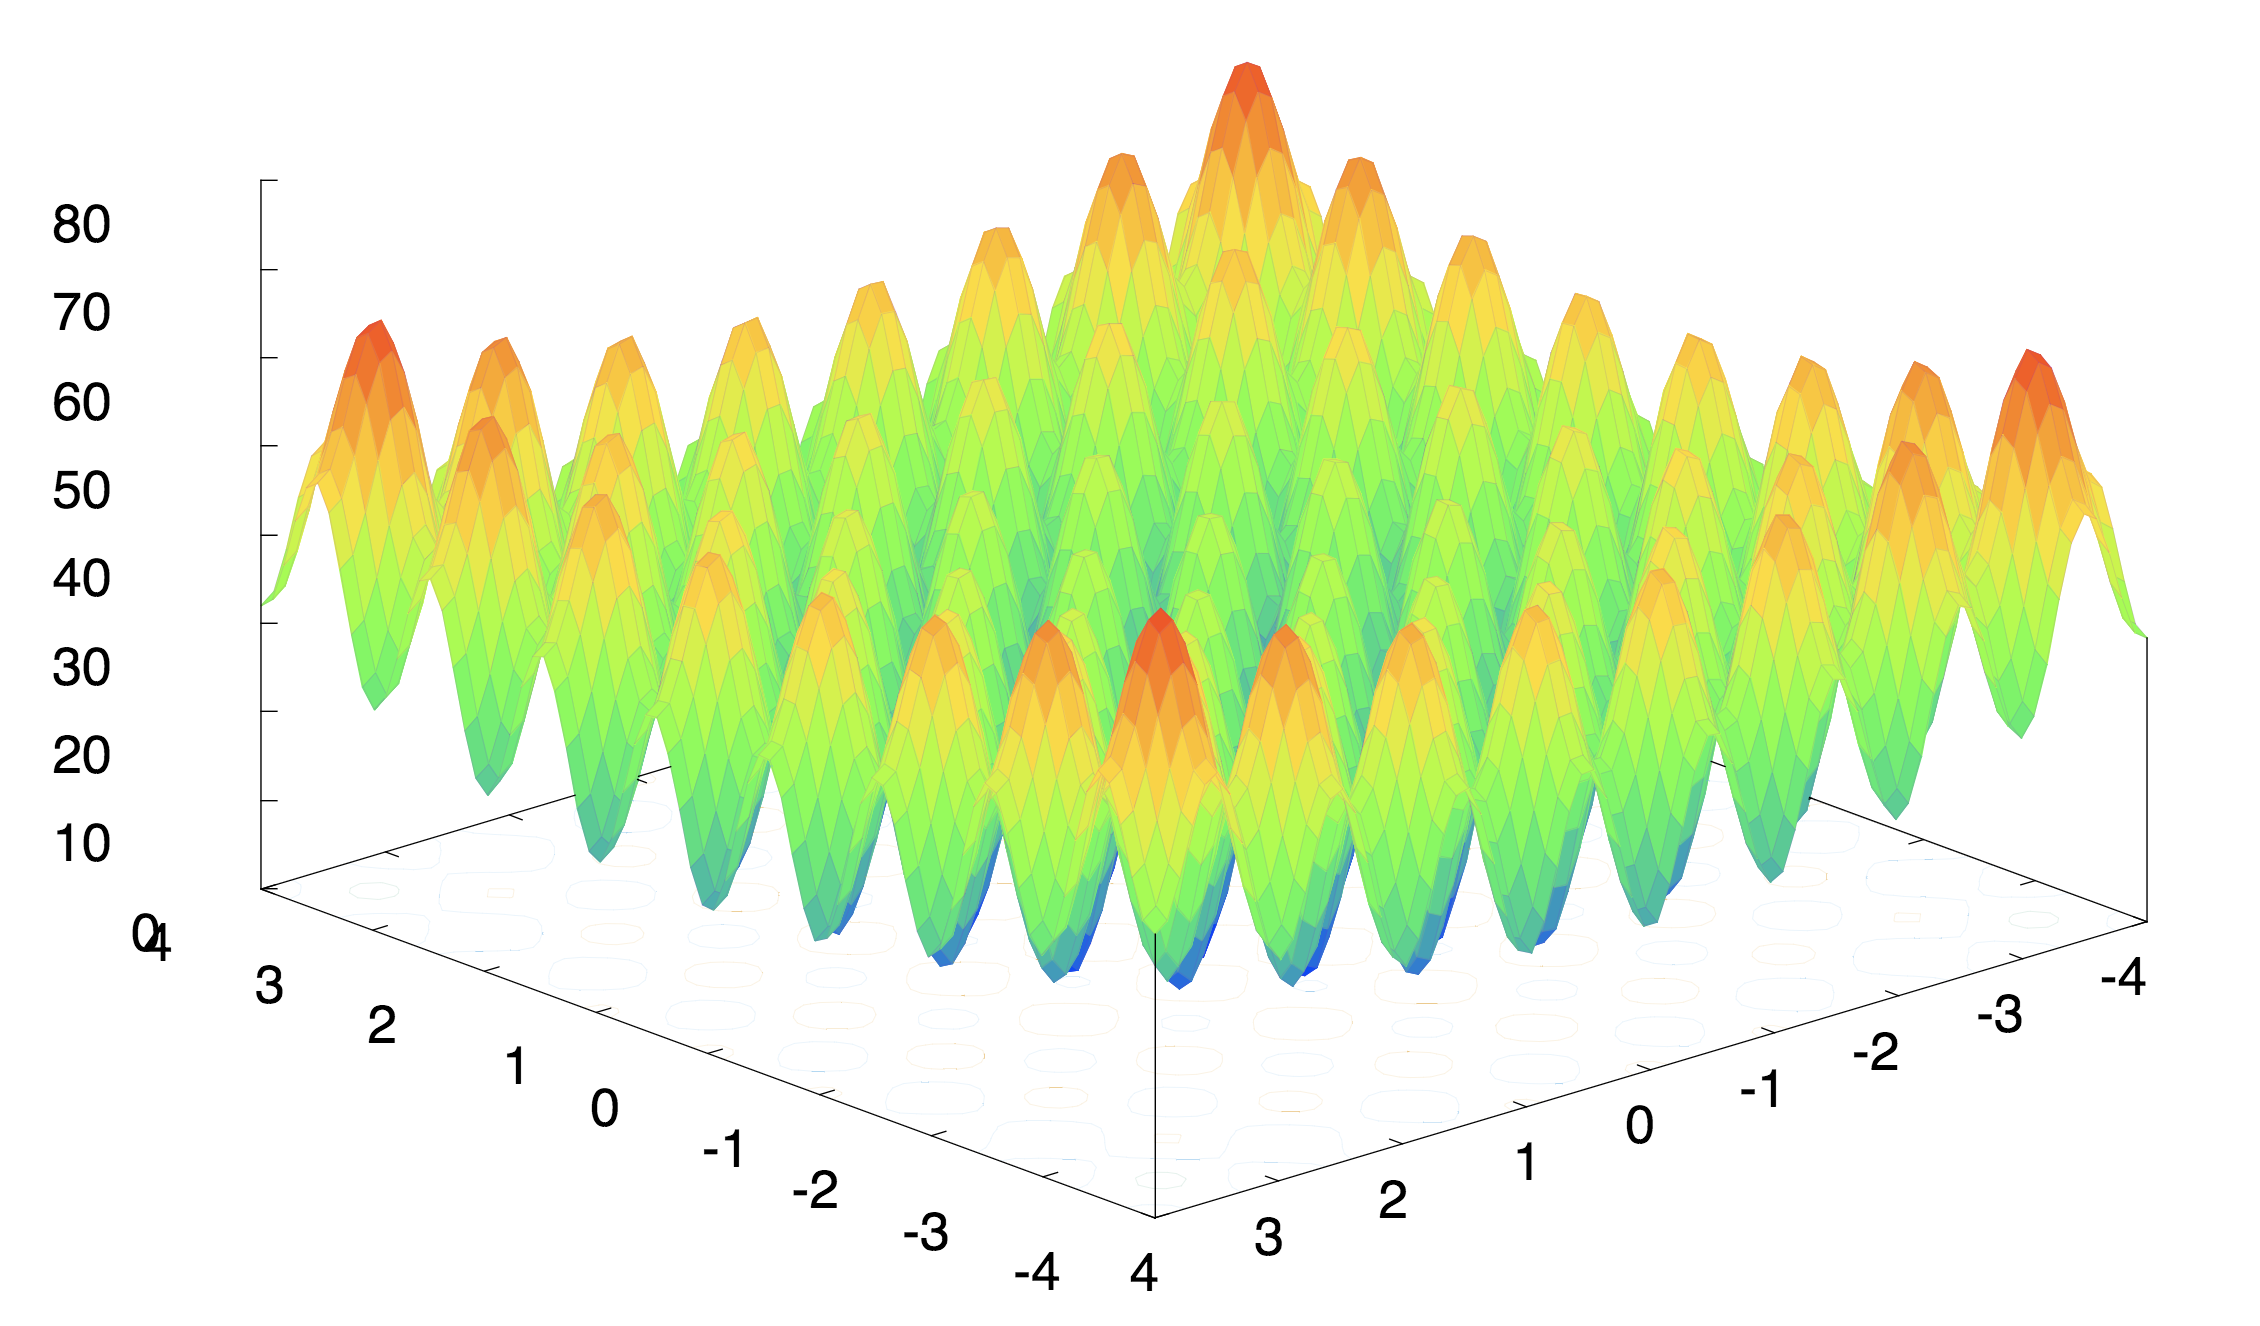
\includegraphics[width=\textwidth]{figures/rastrigin.png}
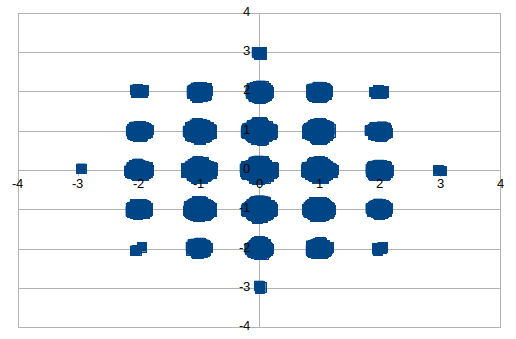
\includegraphics[width=\textwidth]{../20230629_IGN_BigData/figures/oserast6d.png}

%6-D Rastrigin function < 10

}



\sframe{Spatial sensitivity analysis}{



\centering

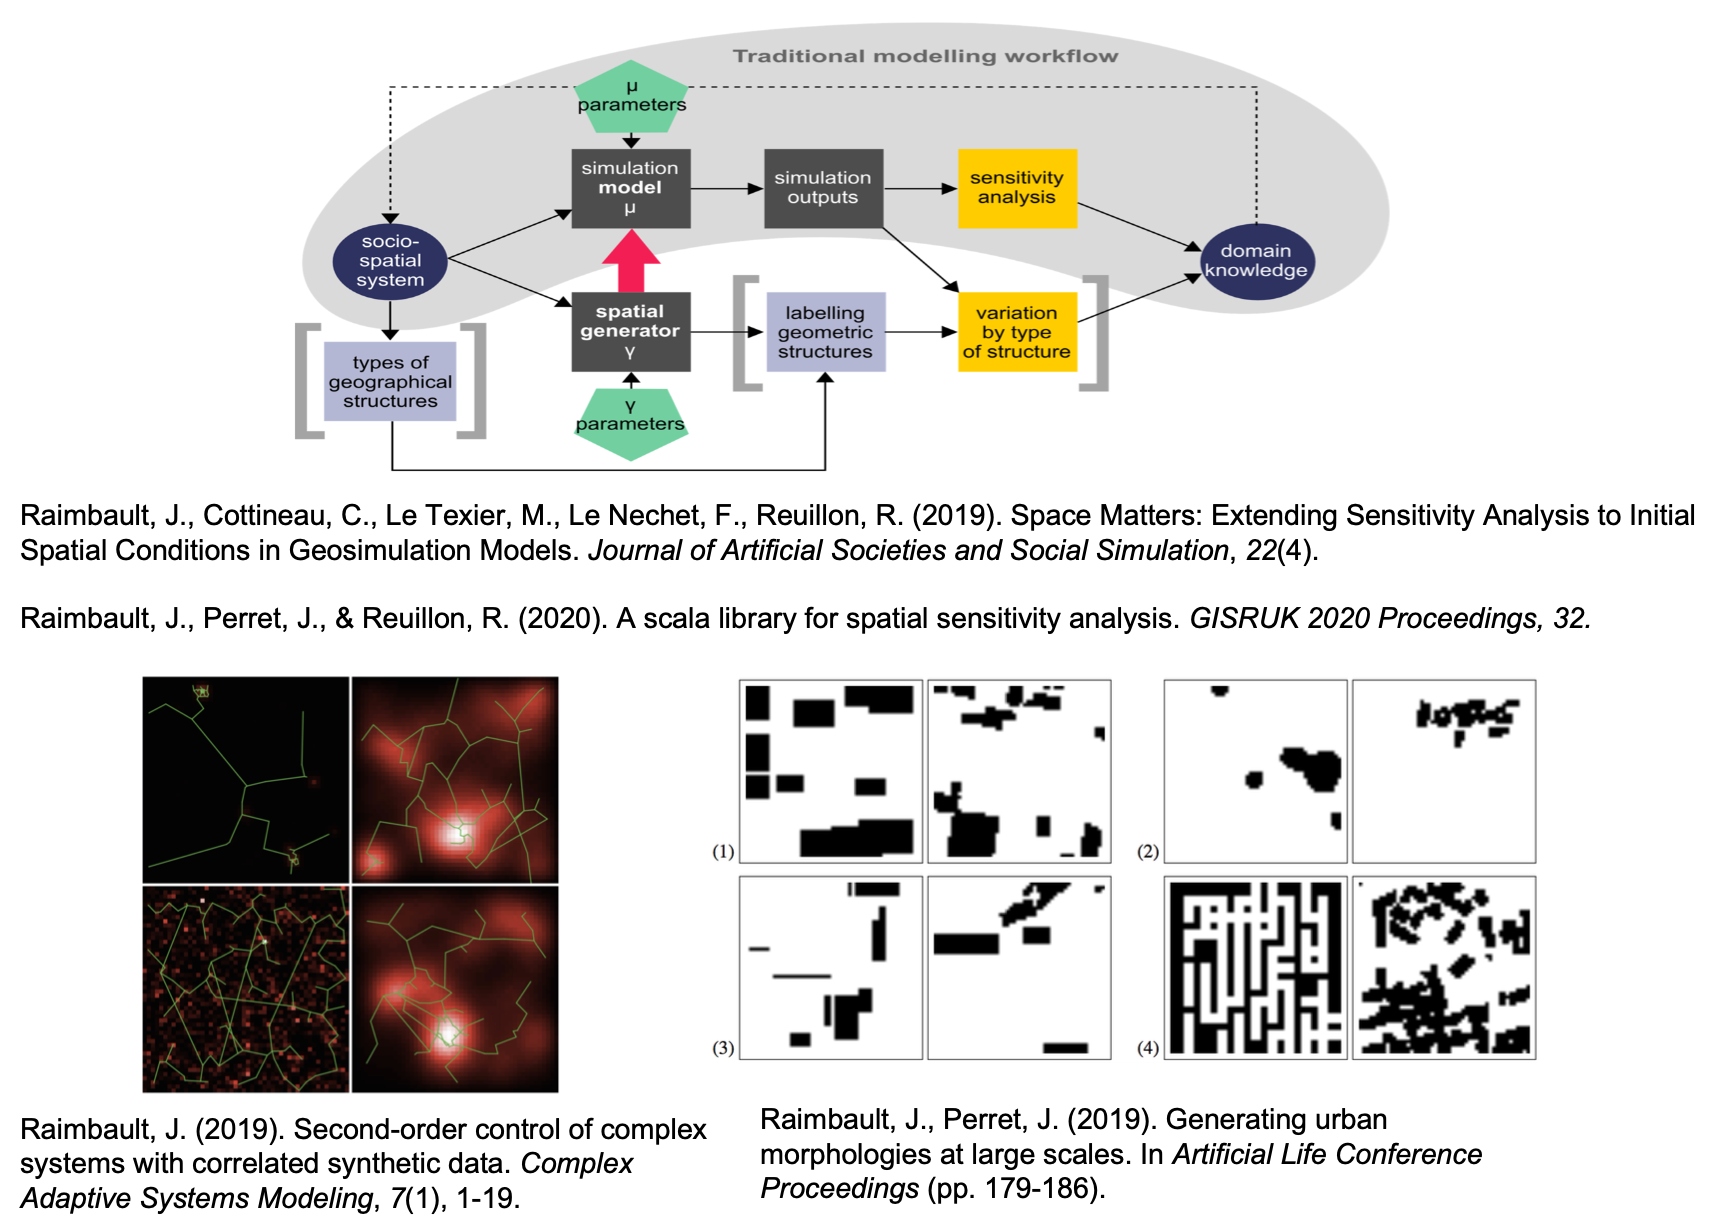
\includegraphics[width=0.95\linewidth]{../20230629_IGN_BigData/figures/spatial_sa.png}

\nocite{raimbault2019second}
\nocite{raimbault2019generating}
\nocite{raimbault2019space}

}




\sframe{Model coupling}{

\justify

\textit{Transport model built using modular and open models}

\bigskip

\textbf{Modèles intégrés :}

\begin{itemize}
	\item MATSim (MATSim Community) for transport \cite{w2016multi}
	\item SPENSER (University of Leeds) for synthetic population \cite{spooner2021dynamic}
	\item QUANT (CASA, University College London) for spatial interactions \cite{batty2021new}
	\item spatialdata library (OpenMOLE community) for spatial data \cite{raimbault2020scala}
\end{itemize}

\smallskip

\tiny

Raimbault, J., \& Batty, M. (2021). Estimating public transport congestion in UK urban areas with open transport models. GISRUK 2021 Proceedings.

\nocite{raimbault2021estimating}

}


\sframe{Model coupling: urbanism and heat island effect}{

\begin{columns}
	\begin{column}{0.6\linewidth}
		\begin{center}
			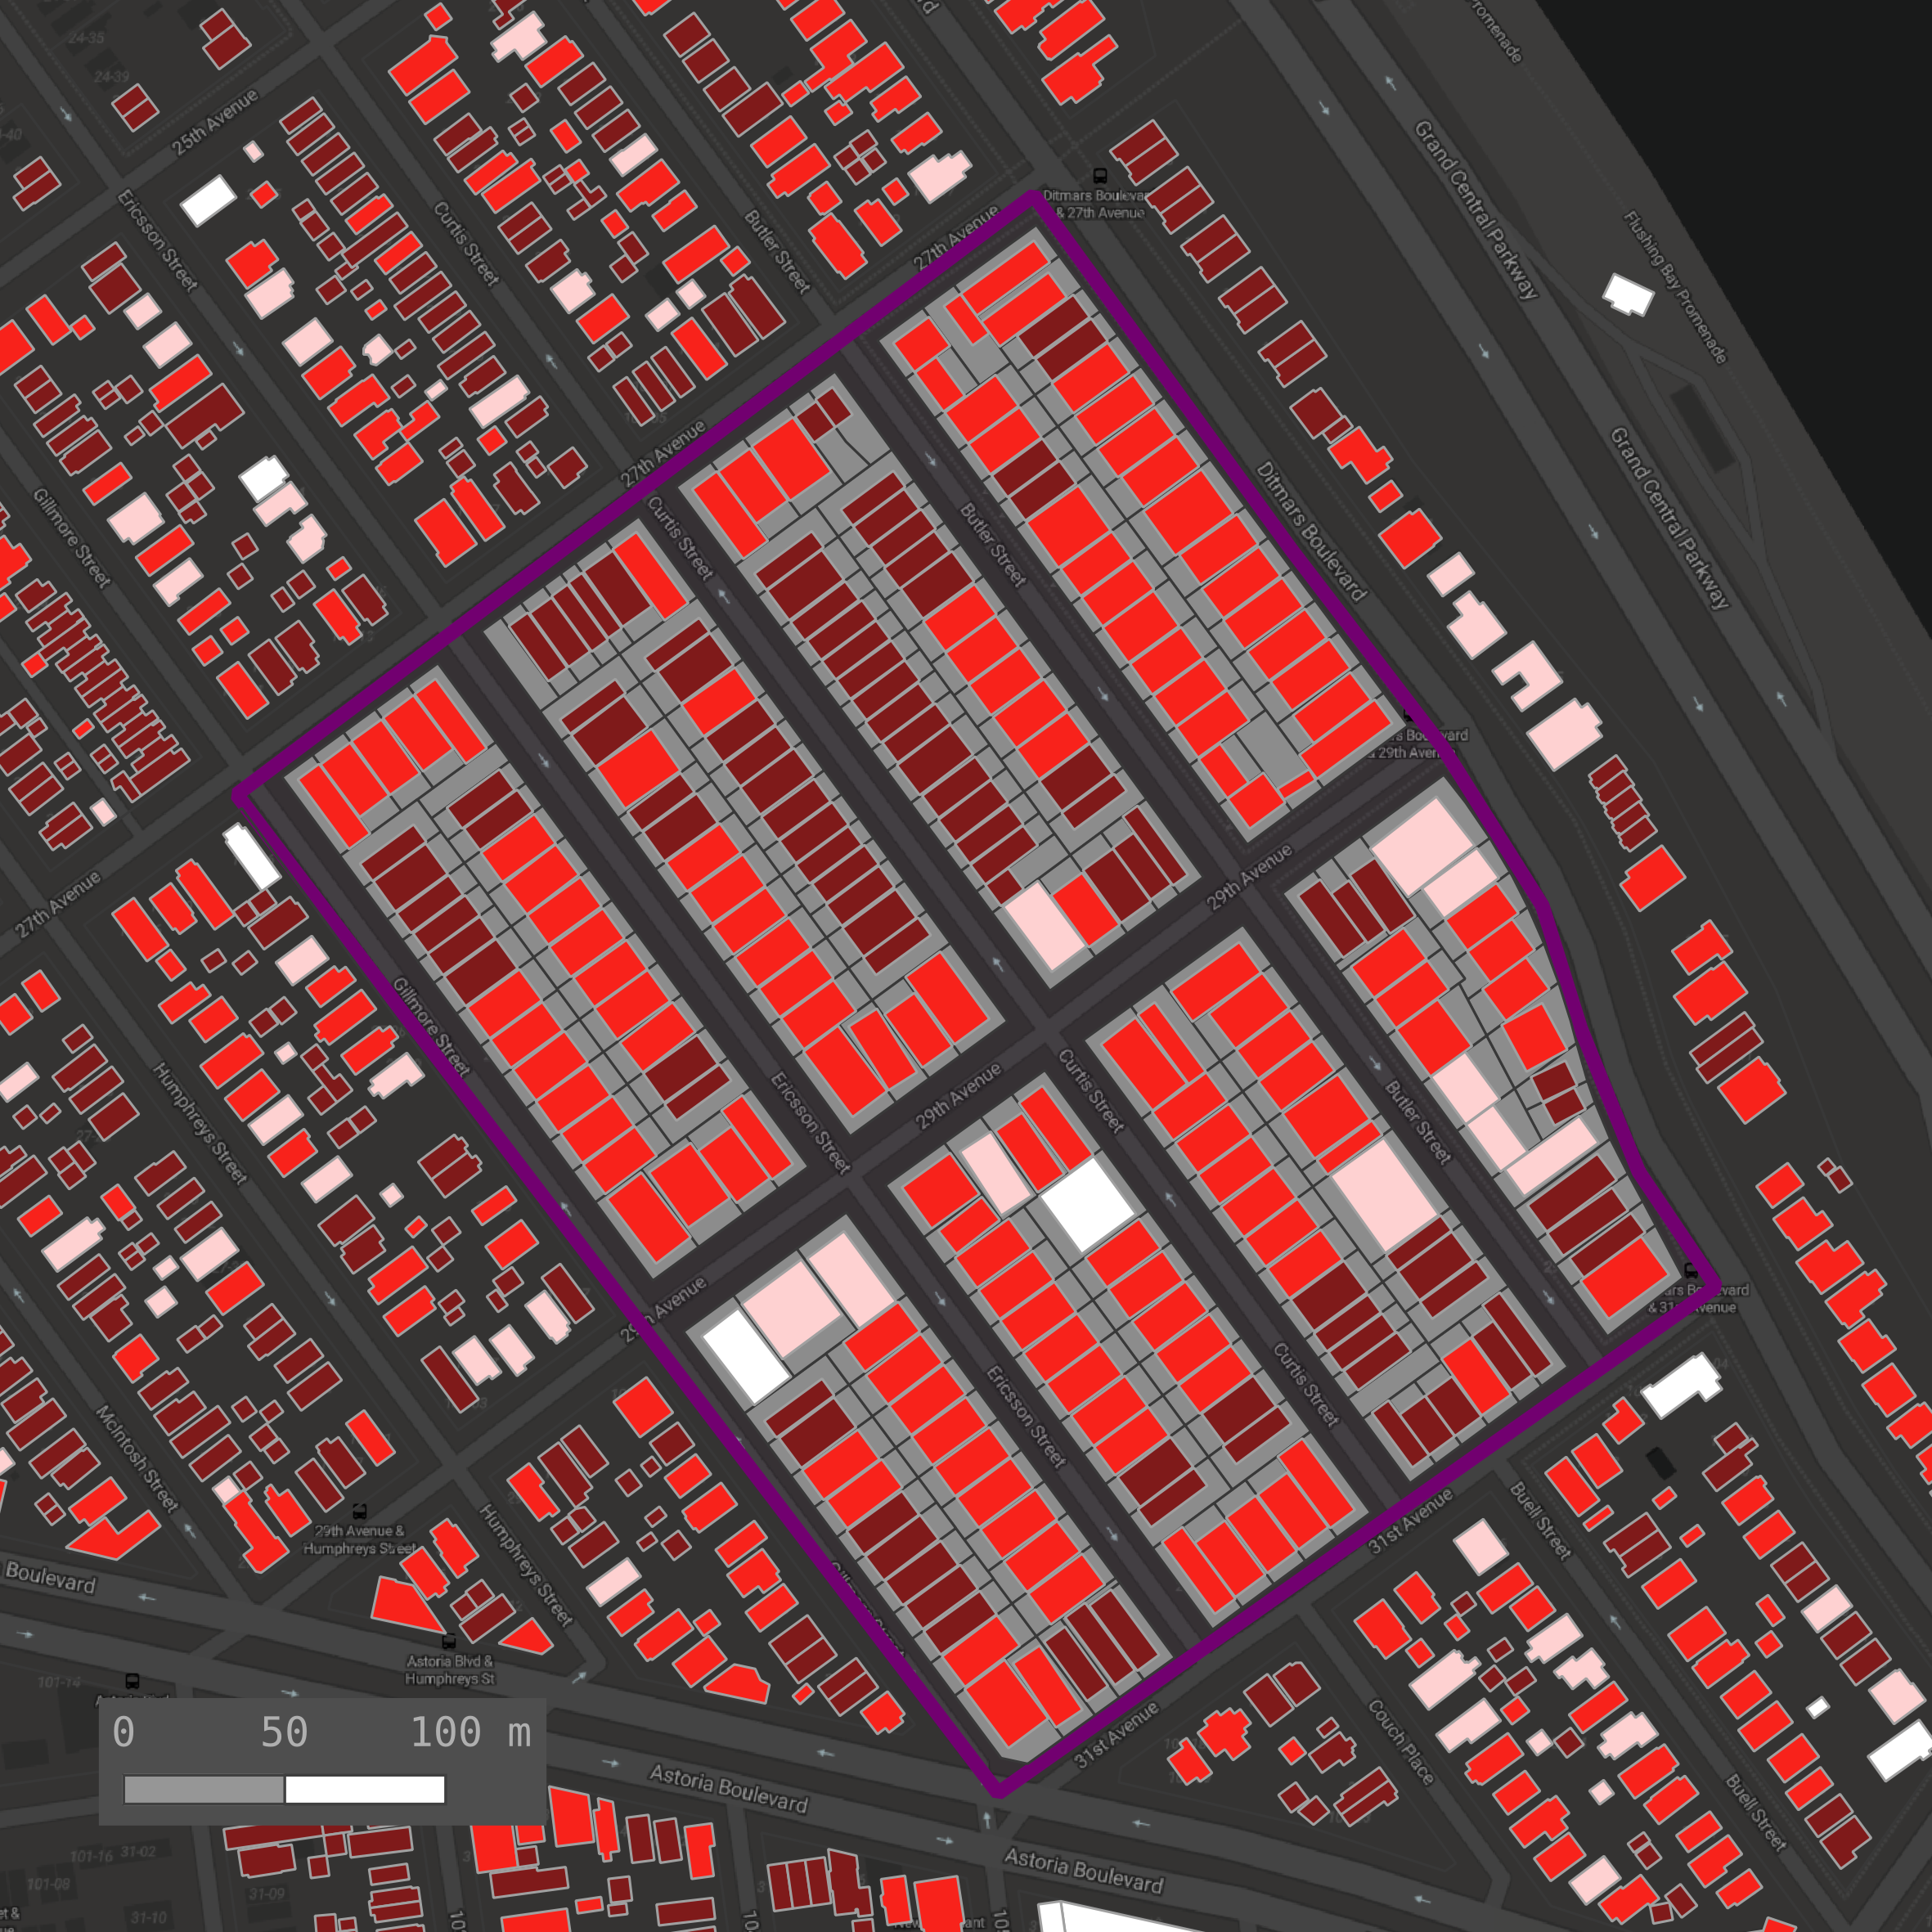
\includegraphics[width=\linewidth]{../20230629_IGN_BigData/figures/buildings_6.png}	
		\end{center}
	\end{column}
	\begin{column}{0.39\linewidth}
		\justify
		\textbf{SURe project} (ASTIG, ISC-PIF, EPIDAPO collaboration)
		
		\bigskip
		
		$\rightarrow$ coupling the SimPLU3D model \cite{brasebin2017apports} with an UHI model.

	\end{column}
\end{columns}




}



\sframe{Model coupling: towards multi-scale models}{



\begin{center}
	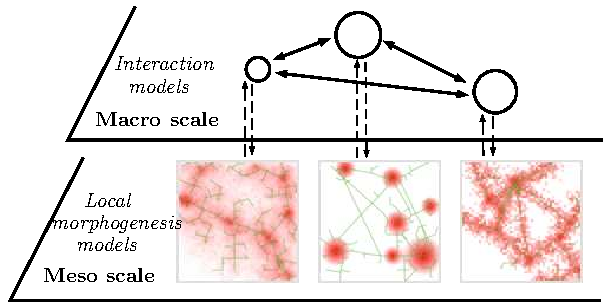
\includegraphics[width=0.75\textwidth]{../20230629_IGN_BigData/figures/multiscale_morph.pdf}
\end{center}

\medskip

\textit{Processes specific to scales, coupling requires a dedicated ontology.} 

\medskip

\tiny

Raimbault, J. (2021). Strong coupling between scales in a multi-scalar model of urban dynamics. arXiv preprint arXiv:2101.12725.

\nocite{raimbault2021strong}

\smallskip

Raimbault, J. (2021). A multiscale model of urban morphogenesis. arXiv preprint arXiv:2103.17241.

\nocite{raimbault2021multiscale}

\smallskip

Raimbault, J. and Pumain, D. (2023). Innovation dynamics in multi-scalar systems of cities. \textit{ALIFE 2023}.


}



\sframe{Synthesis: OpenMOLE benchmark}{

\centering

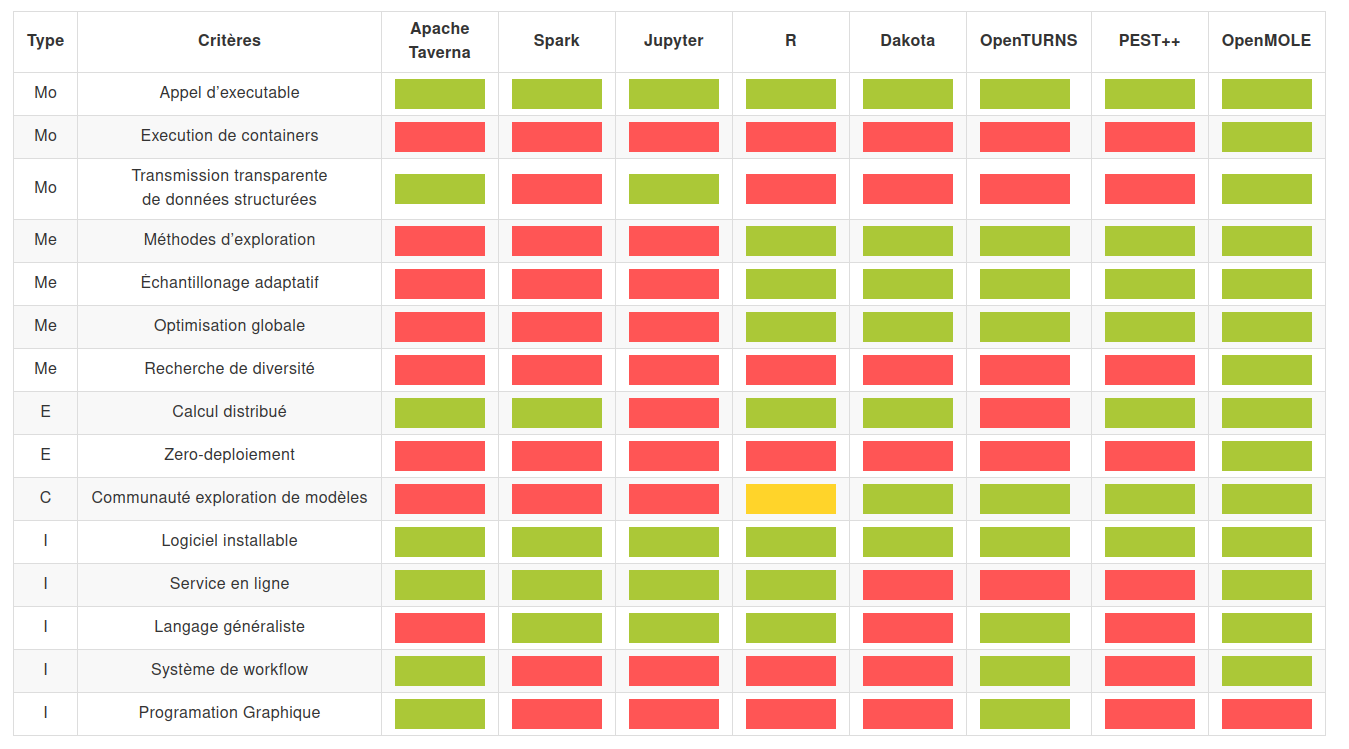
\includegraphics[width=\textwidth]{../20230629_IGN_BigData/figures/openmole_benchmark.png}

}



\sframe{Use OpenMOLE}{

% use -> download, compile, doc ; openmole.org github.com/openmole/openmole

\begin{center}
	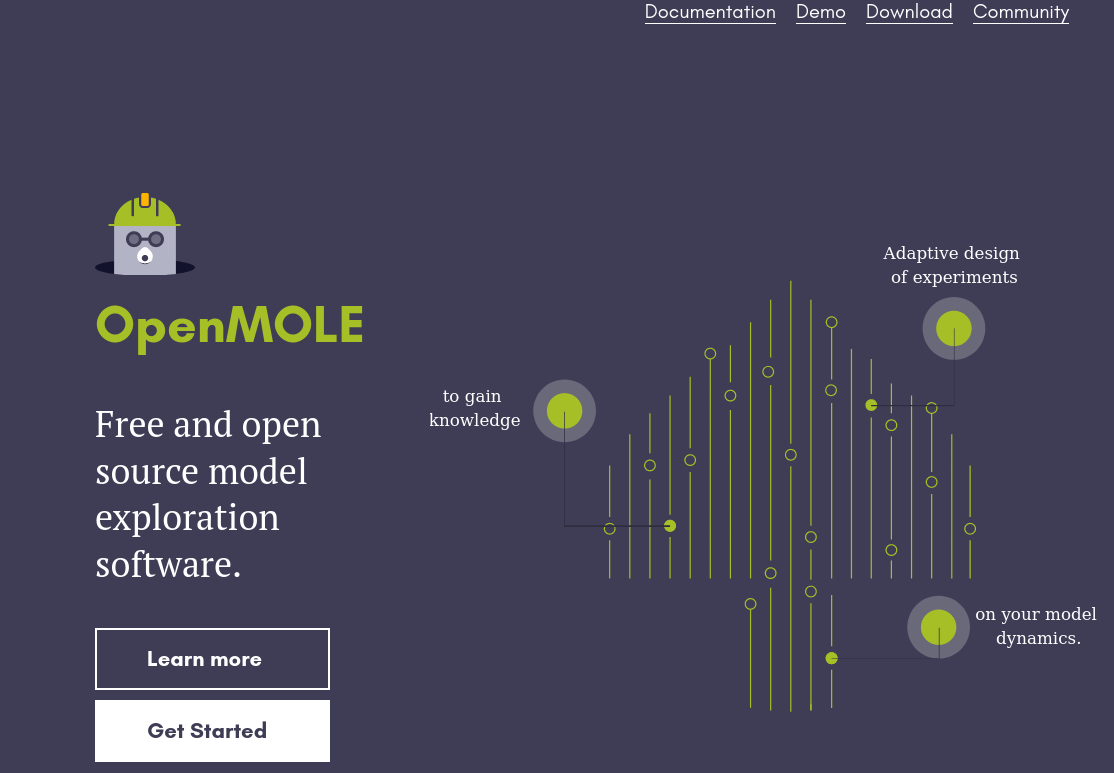
\includegraphics[width=0.7\textwidth]{../20230629_IGN_BigData/figures/website.png}
\end{center}

\smallskip

\footnotesize

$\rightarrow$ Java executable without installation at \texttt{https://openmole.org}, code source to compile at \texttt{https://github.com/openmole/openmole}

$\rightarrow$ Setup an online instance

}

\sframe{Help and contribution}{

% use / contribute : chat- - active community - coding camp

\begin{center}
	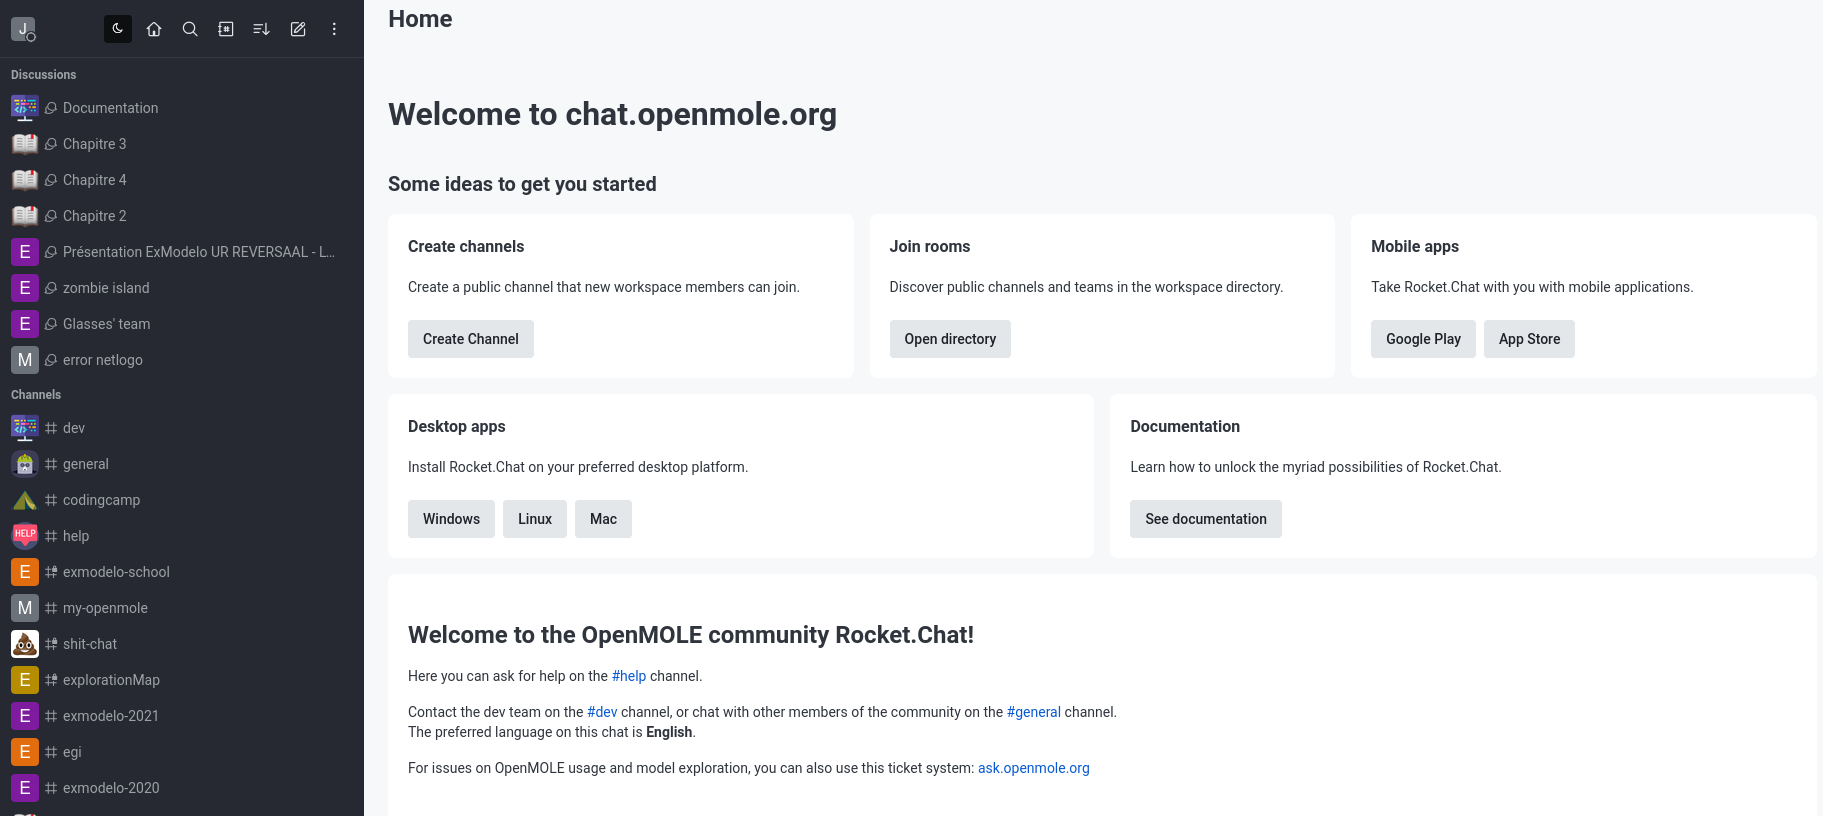
\includegraphics[width=\textwidth]{../20230629_IGN_BigData/figures/chat.png}
\end{center}

\smallskip

Very reactive chat: \texttt{https://chat.openmole.org}



}

\sframe{Contribution}{


\begin{center}
	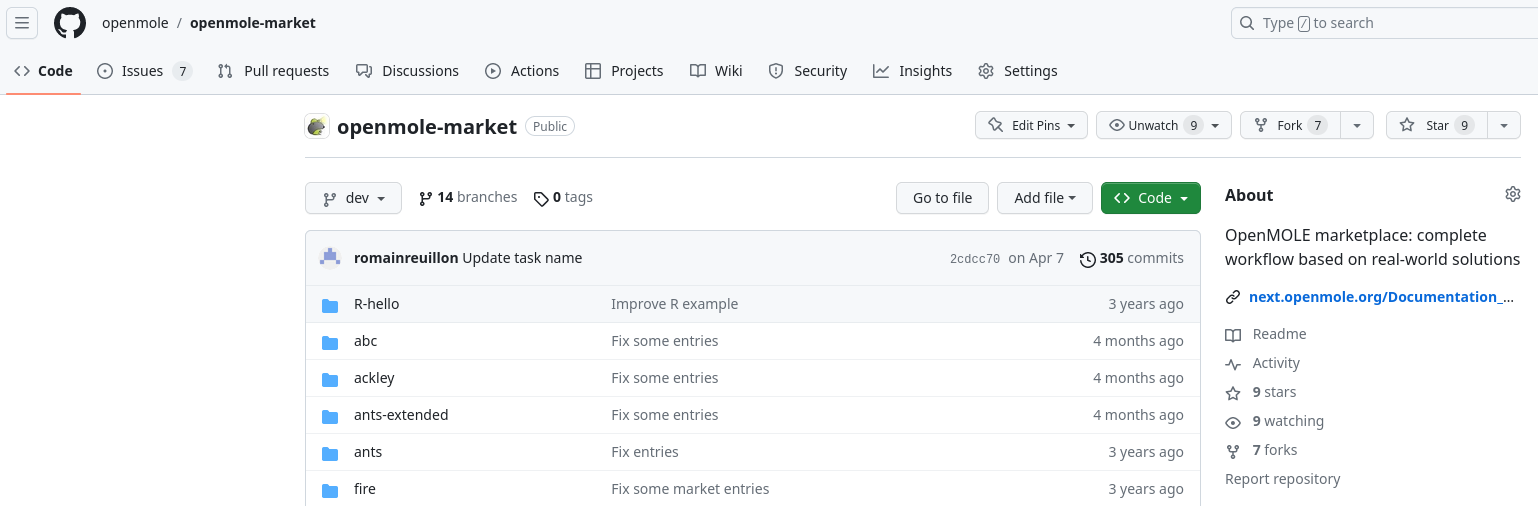
\includegraphics[width=0.9\textwidth]{../20230629_IGN_BigData/figures/market_gh.png}\\\bigskip
	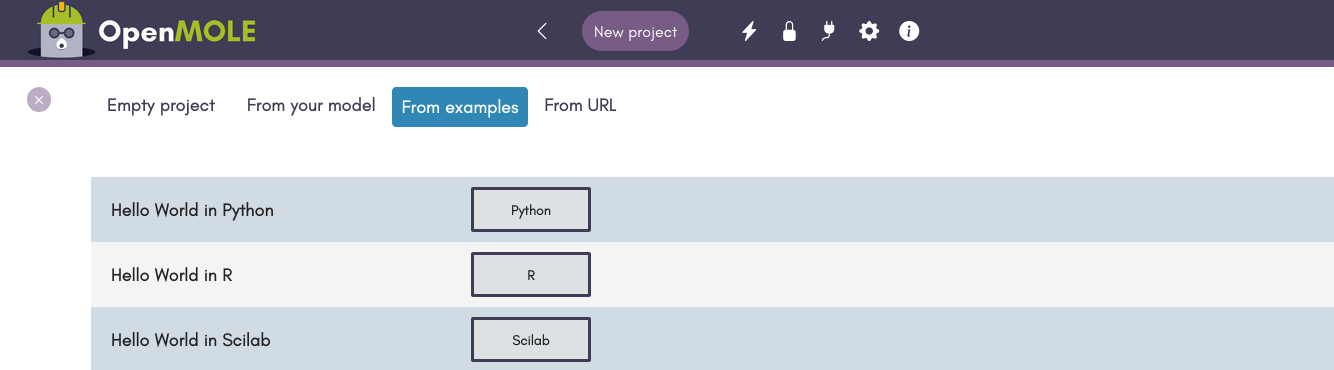
\includegraphics[width=0.9\textwidth]{../20230629_IGN_BigData/figures/market_gui.png}
\end{center}

\bigskip

Add thematic example to the script market \texttt{https://github.com/openmole/openmole-market}

}

\sframe{Learning}{

% learn: exmodelo


\begin{center}
	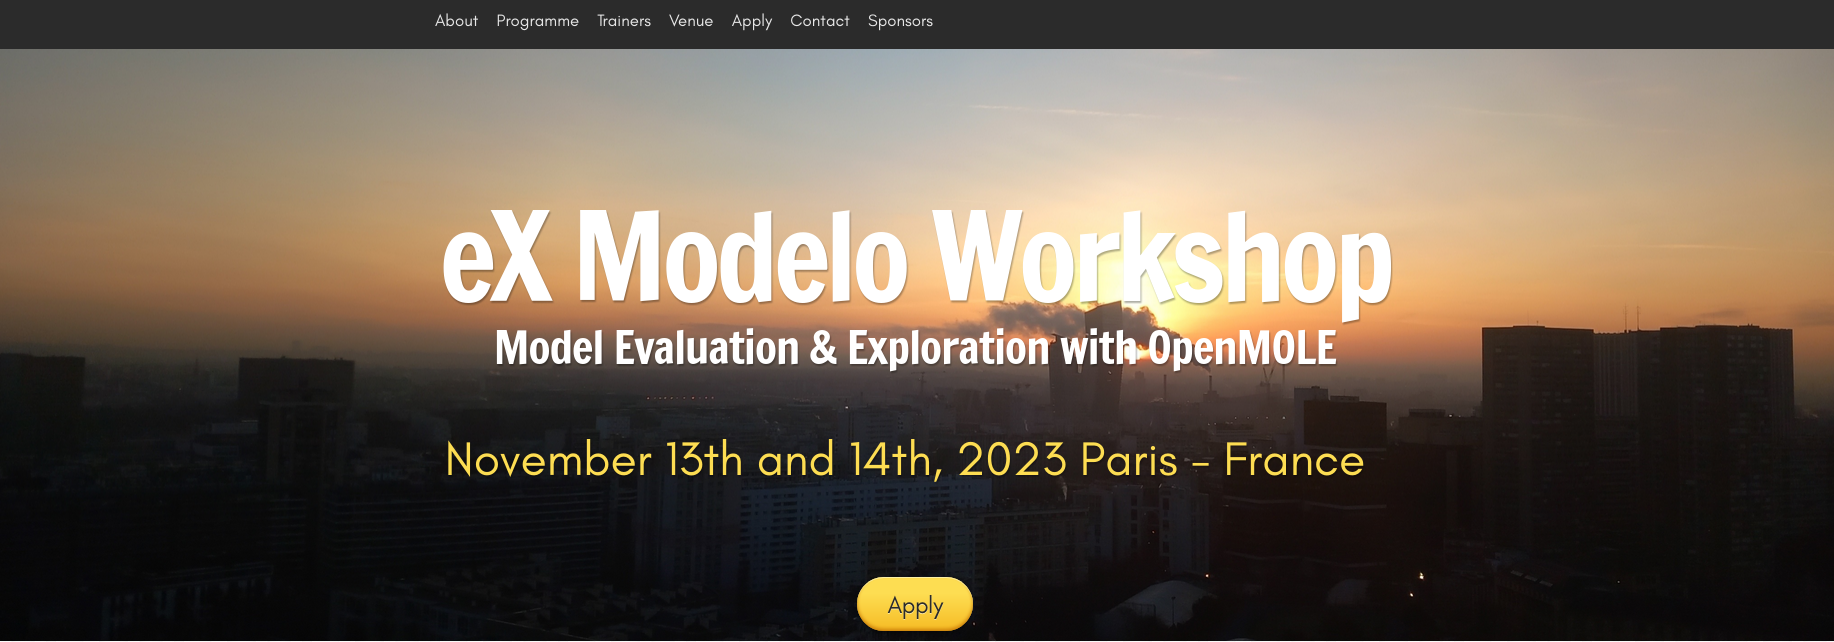
\includegraphics[width=\textwidth]{../20230629_IGN_BigData/figures/exmodelo.png}
\end{center}

\medskip

Learning two days workshop (ISC-PIF, November) \texttt{https://workshop.exmodelo.org/}: applications open



}

\sframe{R{\&}D and scientific consulting}{

\begin{center}
	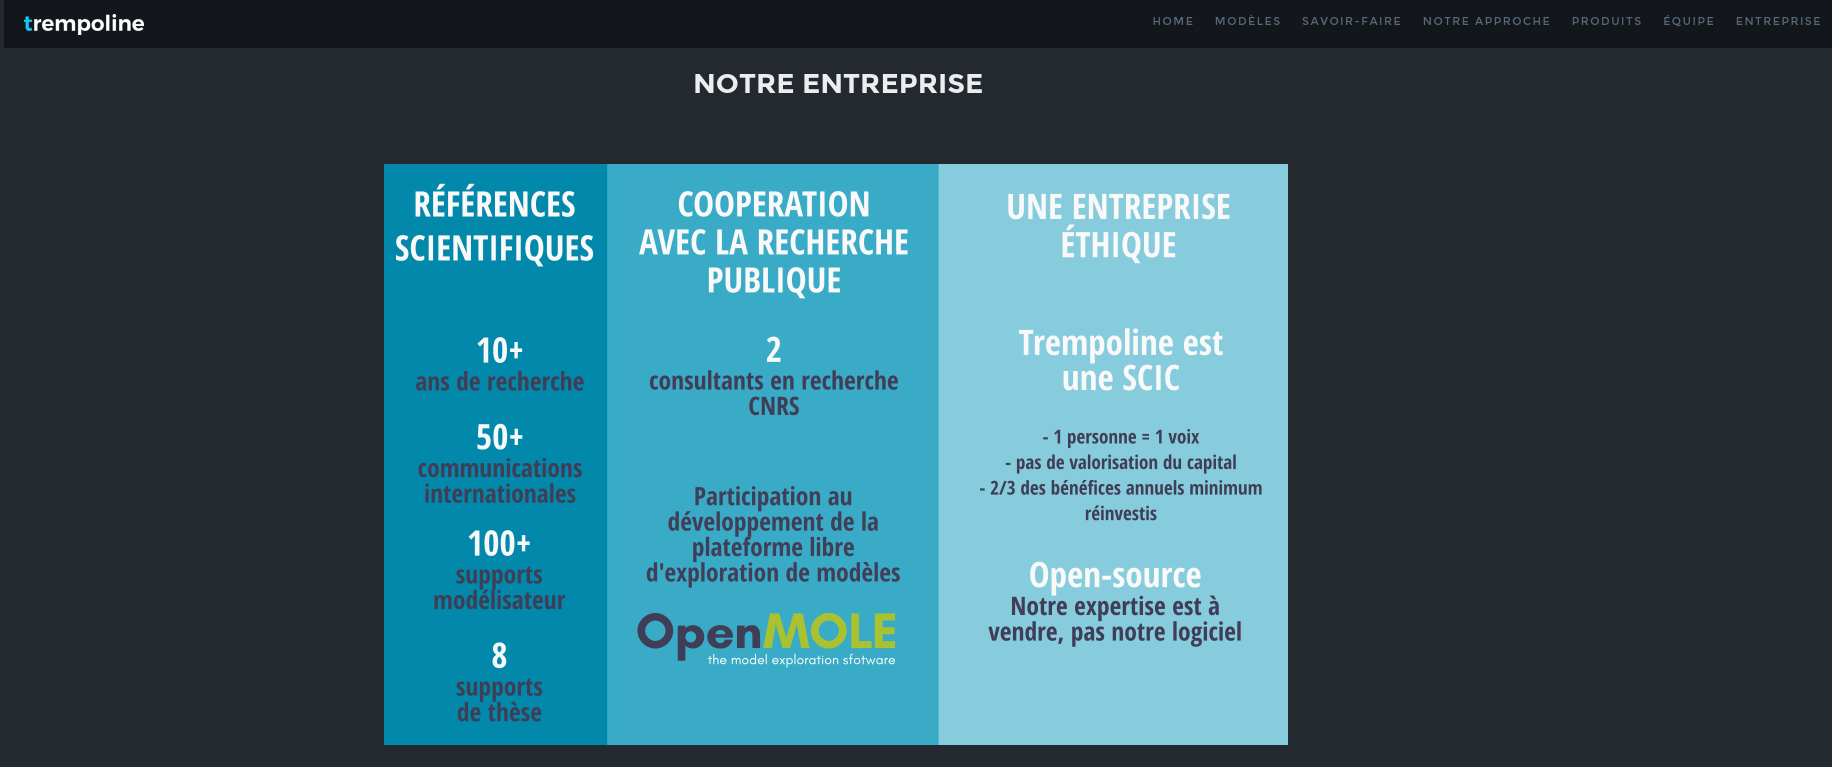
\includegraphics[width=\textwidth]{../20230629_IGN_BigData/figures/trempoline.png}
\end{center}

\medskip

\texttt{https://trempoline.io/}


}



\sframe{Summary of OpenMOLE positioning}{

\textit{A qualitative shift in knowledge that can be extracted from a simulation model with model exploration methods.}

\medskip

Application in different disciplines: Geography \cite{schmitt2014half}\cite{10.1371/journal.pone.0138212}, Ecological modeling \cite{lavallee2018dynamical}, epidemiology \cite{arduin2018modelisation}, etc.



\medskip

\textbf{Main characteristics: }

$\rightarrow$ Complementary role of the three axis: methods, computing environments, model embedding.

$\rightarrow$ Iterative and integrated construction of models and theories.

$\rightarrow$ Model coupling and reproducibility made easy through the scripting language \cite{passerat2017reproducible}.




}







%%%%%%%%%%%%%%%%%%%%%
\begin{frame}[allowframebreaks]
\frametitle{References}
\bibliographystyle{apalike}
\bibliography{biblio,/home/JRaimbault/ComplexSystems/NetworksTerritories/CityNetwork/Biblio/Bibtex/CityNetwork}
\end{frame}
%%%%%%%%%%%%%%%%%%%%%%%%%%%%




\end{document}









